\documentclass[journal]{./IEEEtran/IEEEtran}
%
% If IEEEtran.cls has not been installed into the LaTeX system files,
% manually specify the path to it like:
% \documentclass[journal]{../sty/IEEEtran}

%% Useful packages
\usepackage{amsmath} 
\usepackage{amsfonts}
\usepackage{mathtools} 
\usepackage{graphicx}
\usepackage{bm} % bold math
\usepackage[colorinlistoftodos, textsize=footnotesize]{todonotes}
\usepackage[colorlinks=true, allcolors=blue]{hyperref}
\usepackage{setspace}
%\usepackage{algorithm2e} \usepackage[ruled,vlined]{algorithm2e}
\usepackage{algorithm}% http://ctan.org/pkg/algorithm
\usepackage{algpseudocode}% http://ctan.org/pkg/algorithmicx
\usepackage{tikz}
\usepackage{verbatim}
\usepackage{xcolor}

% ulem: The package provides an \ul (underline) command which will break over
% line ends; this technique may be used to replace \em (both in that form and as
% the \emph command), so as to make output look as if it comes from a
% typewriter. The package also offers double and wavy underlining, and striking
% out (line through words) and crossing out (/// over words).
\usepackage[normalem]{ulem}

\usepackage[thinc]{esdiff}

% amsthm provides the proof environment. 
% N.B. this MUST go before the \newtheorem below. Do not change the order.
\usepackage{amsthm}
% Theorems numbered on a per section basis.
\newtheorem{theorem}{Theorem}[section]
\newtheorem{corollary}{Corollary}[theorem]
\newtheorem{lemma}{Lemma}[section]

\newif\ifcompile
%\compiletrue % uncomment out to compile

\newtheorem{remark}{Remark}

\DeclareMathOperator*{\argmin}{arg\,min}

\newcommand{\RedHighlight}[1]{{\color{red}\textbf{#1}}}

% Super short aliases to color indexes in matrices.
\newcommand{\rr}[1]{{\color{red}#1}} \newcommand{\cc}[1]{{\color{cyan}#1}}

% TikZ commands for drawing schematics.
\newcommand{\tikzmark}[1]{\tikz[overlay, remember picture] \coordinate (#1);}

%For making diagonal entries in a matrix.
\newcommand{\diagentry}[1]{\mathmakebox[1.8em]{#1}}

% Helper to create entries of the form Jₚₜ₁ᵀGₚJₚₜ₂ p = #1 t1 = #2 t2 = #3
\newcommand{\JTGJ}[3]{\mf{J}_{\rr{#1}\cc{#2}}^T\mf{G}_\rr{#1}\mf{J}_{\rr{#1}\cc{#3}}}

\newcommand{\bgamma}{{\bm\gamma}} 
\newcommand{\btgamma}{{\bm{\tilde\gamma}}}
\newcommand{\bsigma}{{\bm\sigma}}


% Vector Font. For 3D vectors.
\newcommand{\vf}[1]{{\bm{#1}}}

% Matrix Font, for matrices, arrays and concatenation of 3D vectors.
\newcommand{\mf}[1]{{\mathbf{#1}}}

% Math shortcuts.
% Matrices:
\newcommand{\sM}{\mf{M}}
\newcommand{\sJ}{\mf{J}}
\newcommand{\sJT}{\mf{J}^T}
\newcommand{\sJbar}{\bar{\mf{J}}}
\newcommand{\sJbarT}{\bar{\mf{J}}^T}
\newcommand{\sB}{\mf{B}}
\newcommand{\sBT}{\mf{B}^T}
\newcommand{\sG}{\mf{G}}
\newcommand{\sGT}{\mf{G}^T}
\newcommand{\sR}{\mf{R}}
\newcommand{\sRinv}{\mf{R}^{-1}}
\newcommand{\ssqrtR}{\mf{R}^{1/2}}
\newcommand{\ssqrtRinv}{\mf{R}^{-1/2}}
% Vectors
\newcommand{\sthat}{\hat{\vf{t}}}
% Projections:
% gradient of gamma with respect to y.
\newcommand{\sP}{\mf{P}}
% gradient of gamma_tilde with respect to y_tilde.
\newcommand{\sGtilde}{\tilde{\mf{G}}} 
\newcommand{\sPt}{\mf{P}_t}

\newcommand{\smalltodo}[2][]
{\todo[caption={#2}, #1] {\begin{spacing}{0.5}#2\end{spacing}}}

\newcommand{\ShermComment}[2][]{\smalltodo[color=blue!40, author=Sherm,
#1]{#2}{}}

\newcommand{\EvanComment}[2][]{\smalltodo[color=green!40, author=Evan,
	#1]{#2}{}}

\newcommand{\SeanComment}[2][]{\smalltodo[color=cyan!40, author=Sean, #1]{#2}{}}

\newcommand{\PaulComment}[2][]{\smalltodo[color=magenta!40, author=Paul,
	#1]{#2}{}}



% Some very useful LaTeX packages include:
% (uncomment the ones you want to load)


% *** MISC UTILITY PACKAGES ***
%
%\usepackage{ifpdf}
% Heiko Oberdiek's ifpdf.sty is very useful if you need conditional
% compilation based on whether the output is pdf or dvi.
% usage:
% \ifpdf
%   % pdf code
% \else
%   % dvi code
% \fi
% The latest version of ifpdf.sty can be obtained from:
% http://www.ctan.org/pkg/ifpdf
% Also, note that IEEEtran.cls V1.7 and later provides a builtin
% \ifCLASSINFOpdf conditional that works the same way.
% When switching from latex to pdflatex and vice-versa, the compiler may
% have to be run twice to clear warning/error messages.






% *** CITATION PACKAGES ***
%
%\usepackage{cite}
% cite.sty was written by Donald Arseneau
% V1.6 and later of IEEEtran pre-defines the format of the cite.sty package
% \cite{} output to follow that of the IEEE. Loading the cite package will
% result in citation numbers being automatically sorted and properly
% "compressed/ranged". e.g., [1], [9], [2], [7], [5], [6] without using
% cite.sty will become [1], [2], [5]--[7], [9] using cite.sty. cite.sty's
% \cite will automatically add leading space, if needed. Use cite.sty's
% noadjust option (cite.sty V3.8 and later) if you want to turn this off
% such as if a citation ever needs to be enclosed in parenthesis.
% cite.sty is already installed on most LaTeX systems. Be sure and use
% version 5.0 (2009-03-20) and later if using hyperref.sty.
% The latest version can be obtained at:
% http://www.ctan.org/pkg/cite
% The documentation is contained in the cite.sty file itself.






% *** GRAPHICS RELATED PACKAGES ***
%
\ifCLASSINFOpdf
  % \usepackage[pdftex]{graphicx}
  % declare the path(s) where your graphic files are
  % \graphicspath{{../pdf/}{../jpeg/}}
  % and their extensions so you won't have to specify these with
  % every instance of \includegraphics
  % \DeclareGraphicsExtensions{.pdf,.jpeg,.png}
\else
  % or other class option (dvipsone, dvipdf, if not using dvips). graphicx
  % will default to the driver specified in the system graphics.cfg if no
  % driver is specified.
  % \usepackage[dvips]{graphicx}
  % declare the path(s) where your graphic files are
  % \graphicspath{{../eps/}}
  % and their extensions so you won't have to specify these with
  % every instance of \includegraphics
  % \DeclareGraphicsExtensions{.eps}
\fi
% graphicx was written by David Carlisle and Sebastian Rahtz. It is
% required if you want graphics, photos, etc. graphicx.sty is already
% installed on most LaTeX systems. The latest version and documentation
% can be obtained at: 
% http://www.ctan.org/pkg/graphicx
% Another good source of documentation is "Using Imported Graphics in
% LaTeX2e" by Keith Reckdahl which can be found at:
% http://www.ctan.org/pkg/epslatex
%
% latex, and pdflatex in dvi mode, support graphics in encapsulated
% postscript (.eps) format. pdflatex in pdf mode supports graphics
% in .pdf, .jpeg, .png and .mps (metapost) formats. Users should ensure
% that all non-photo figures use a vector format (.eps, .pdf, .mps) and
% not a bitmapped formats (.jpeg, .png). The IEEE frowns on bitmapped formats
% which can result in "jaggedy"/blurry rendering of lines and letters as
% well as large increases in file sizes.
%
% You can find documentation about the pdfTeX application at:
% http://www.tug.org/applications/pdftex





% *** MATH PACKAGES ***
%
%\usepackage{amsmath}
% A popular package from the American Mathematical Society that provides
% many useful and powerful commands for dealing with mathematics.
%
% Note that the amsmath package sets \interdisplaylinepenalty to 10000
% thus preventing page breaks from occurring within multiline equations. Use:
%\interdisplaylinepenalty=2500
% after loading amsmath to restore such page breaks as IEEEtran.cls normally
% does. amsmath.sty is already installed on most LaTeX systems. The latest
% version and documentation can be obtained at:
% http://www.ctan.org/pkg/amsmath





% *** SPECIALIZED LIST PACKAGES ***
%
%\usepackage{algorithmic}
% algorithmic.sty was written by Peter Williams and Rogerio Brito.
% This package provides an algorithmic environment fo describing algorithms.
% You can use the algorithmic environment in-text or within a figure
% environment to provide for a floating algorithm. Do NOT use the algorithm
% floating environment provided by algorithm.sty (by the same authors) or
% algorithm2e.sty (by Christophe Fiorio) as the IEEE does not use dedicated
% algorithm float types and packages that provide these will not provide
% correct IEEE style captions. The latest version and documentation of
% algorithmic.sty can be obtained at:
% http://www.ctan.org/pkg/algorithms
% Also of interest may be the (relatively newer and more customizable)
% algorithmicx.sty package by Szasz Janos:
% http://www.ctan.org/pkg/algorithmicx




% *** ALIGNMENT PACKAGES ***
%
%\usepackage{array}
% Frank Mittelbach's and David Carlisle's array.sty patches and improves
% the standard LaTeX2e array and tabular environments to provide better
% appearance and additional user controls. As the default LaTeX2e table
% generation code is lacking to the point of almost being broken with
% respect to the quality of the end results, all users are strongly
% advised to use an enhanced (at the very least that provided by array.sty)
% set of table tools. array.sty is already installed on most systems. The
% latest version and documentation can be obtained at:
% http://www.ctan.org/pkg/array


% IEEEtran contains the IEEEeqnarray family of commands that can be used to
% generate multiline equations as well as matrices, tables, etc., of high
% quality.




% *** SUBFIGURE PACKAGES ***
%\ifCLASSOPTIONcompsoc
%  \usepackage[caption=false,font=normalsize,labelfont=sf,textfont=sf]{subfig}
%\else
%  \usepackage[caption=false,font=footnotesize]{subfig}
%\fi
% subfig.sty, written by Steven Douglas Cochran, is the modern replacement
% for subfigure.sty, the latter of which is no longer maintained and is
% incompatible with some LaTeX packages including fixltx2e. However,
% subfig.sty requires and automatically loads Axel Sommerfeldt's caption.sty
% which will override IEEEtran.cls' handling of captions and this will result
% in non-IEEE style figure/table captions. To prevent this problem, be sure
% and invoke subfig.sty's "caption=false" package option (available since
% subfig.sty version 1.3, 2005/06/28) as this is will preserve IEEEtran.cls
% handling of captions.
% Note that the Computer Society format requires a larger sans serif font
% than the serif footnote size font used in traditional IEEE formatting
% and thus the need to invoke different subfig.sty package options depending
% on whether compsoc mode has been enabled.
%
% The latest version and documentation of subfig.sty can be obtained at:
% http://www.ctan.org/pkg/subfig




% *** FLOAT PACKAGES ***
%
%\usepackage{fixltx2e}
% fixltx2e, the successor to the earlier fix2col.sty, was written by
% Frank Mittelbach and David Carlisle. This package corrects a few problems
% in the LaTeX2e kernel, the most notable of which is that in current
% LaTeX2e releases, the ordering of single and double column floats is not
% guaranteed to be preserved. Thus, an unpatched LaTeX2e can allow a
% single column figure to be placed prior to an earlier double column
% figure.
% Be aware that LaTeX2e kernels dated 2015 and later have fixltx2e.sty's
% corrections already built into the system in which case a warning will
% be issued if an attempt is made to load fixltx2e.sty as it is no longer
% needed.
% The latest version and documentation can be found at:
% http://www.ctan.org/pkg/fixltx2e


%\usepackage{stfloats}
% stfloats.sty was written by Sigitas Tolusis. This package gives LaTeX2e
% the ability to do double column floats at the bottom of the page as well
% as the top. (e.g., "\begin{figure*}[!b]" is not normally possible in
% LaTeX2e). It also provides a command:
%\fnbelowfloat
% to enable the placement of footnotes below bottom floats (the standard
% LaTeX2e kernel puts them above bottom floats). This is an invasive package
% which rewrites many portions of the LaTeX2e float routines. It may not work
% with other packages that modify the LaTeX2e float routines. The latest
% version and documentation can be obtained at:
% http://www.ctan.org/pkg/stfloats
% Do not use the stfloats baselinefloat ability as the IEEE does not allow
% \baselineskip to stretch. Authors submitting work to the IEEE should note
% that the IEEE rarely uses double column equations and that authors should try
% to avoid such use. Do not be tempted to use the cuted.sty or midfloat.sty
% packages (also by Sigitas Tolusis) as the IEEE does not format its papers in
% such ways.
% Do not attempt to use stfloats with fixltx2e as they are incompatible.
% Instead, use Morten Hogholm'a dblfloatfix which combines the features
% of both fixltx2e and stfloats:
%
% \usepackage{dblfloatfix}
% The latest version can be found at:
% http://www.ctan.org/pkg/dblfloatfix




%\ifCLASSOPTIONcaptionsoff
%  \usepackage[nomarkers]{endfloat}
% \let\MYoriglatexcaption\caption
% \renewcommand{\caption}[2][\relax]{\MYoriglatexcaption[#2]{#2}}
%\fi
% endfloat.sty was written by James Darrell McCauley, Jeff Goldberg and 
% Axel Sommerfeldt. This package may be useful when used in conjunction with 
% IEEEtran.cls'  captionsoff option. Some IEEE journals/societies require that
% submissions have lists of figures/tables at the end of the paper and that
% figures/tables without any captions are placed on a page by themselves at
% the end of the document. If needed, the draftcls IEEEtran class option or
% \CLASSINPUTbaselinestretch interface can be used to increase the line
% spacing as well. Be sure and use the nomarkers option of endfloat to
% prevent endfloat from "marking" where the figures would have been placed
% in the text. The two hack lines of code above are a slight modification of
% that suggested by in the endfloat docs (section 8.4.1) to ensure that
% the full captions always appear in the list of figures/tables - even if
% the user used the short optional argument of \caption[]{}.
% IEEE papers do not typically make use of \caption[]'s optional argument,
% so this should not be an issue. A similar trick can be used to disable
% captions of packages such as subfig.sty that lack options to turn off
% the subcaptions:
% For subfig.sty:
% \let\MYorigsubfloat\subfloat
% \renewcommand{\subfloat}[2][\relax]{\MYorigsubfloat[]{#2}}
% However, the above trick will not work if both optional arguments of
% the \subfloat command are used. Furthermore, there needs to be a
% description of each subfigure *somewhere* and endfloat does not add
% subfigure captions to its list of figures. Thus, the best approach is to
% avoid the use of subfigure captions (many IEEE journals avoid them anyway)
% and instead reference/explain all the subfigures within the main caption.
% The latest version of endfloat.sty and its documentation can obtained at:
% http://www.ctan.org/pkg/endfloat
%
% The IEEEtran \ifCLASSOPTIONcaptionsoff conditional can also be used
% later in the document, say, to conditionally put the References on a 
% page by themselves.




% *** PDF, URL AND HYPERLINK PACKAGES ***
%
%\usepackage{url}
% url.sty was written by Donald Arseneau. It provides better support for
% handling and breaking URLs. url.sty is already installed on most LaTeX
% systems. The latest version and documentation can be obtained at:
% http://www.ctan.org/pkg/url
% Basically, \url{my_url_here}.




% *** Do not adjust lengths that control margins, column widths, etc. ***
% *** Do not use packages that alter fonts (such as pslatex).         ***
% There should be no need to do such things with IEEEtran.cls V1.6 and later.
% (Unless specifically asked to do so by the journal or conference you plan
% to submit to, of course. )


% correct bad hyphenation here
\hyphenation{op-tical net-works semi-conduc-tor}


\begin{document}
%
% paper title
% Titles are generally capitalized except for words such as a, an, and, as,
% at, but, by, for, in, nor, of, on, or, the, to and up, which are usually
% not capitalized unless they are the first or last word of the title.
% Linebreaks \\ can be used within to get better formatting as desired.
% Do not put math or special symbols in the title.
\title{An Unconstrained Convex Formulation of Compliant Contact\\
PLEASE DO NOT DISTRIBUTE}
%
%
% author names and IEEE memberships
% note positions of commas and nonbreaking spaces ( ~ ) LaTeX will not break
% a structure at a ~ so this keeps an author's name from being broken across
% two lines.
% use \thanks{} to gain access to the first footnote area
% a separate \thanks must be used for each paragraph as LaTeX2e's \thanks
% was not built to handle multiple paragraphs
%


\author{Alejandro Castro, Frank Permenter, Xuchen Han% <-this % stops a space

%\thanks{Manuscript received: September, 10, 2019; Revised December, 12, 2019; Accepted December, 12, 2019.}
%\thanks{This paper was recommended for publication by Kyu-Jin Cho upon evaluation of the Associate Editor and Reviewers' comments.}
\thanks{All the authors are with Toyota Research Institute, Cambridge, MA, USA, {\tt\small firstname.lastname@tri.global}.}%
%\thanks{Digital Object Identifier (DOI): see top of this page.}
}

% note the % following the last \IEEEmembership and also \thanks - 
% these prevent an unwanted space from occurring between the last author name
% and the end of the author line. i.e., if you had this:
% 
% \author{....lastname \thanks{...} \thanks{...} }
%                     ^------------^------------^----Do not want these spaces!
%
% a space would be appended to the last name and could cause every name on that
% line to be shifted left slightly. This is one of those "LaTeX things". For
% instance, "\textbf{A} \textbf{B}" will typeset as "A B" not "AB". To get
% "AB" then you have to do: "\textbf{A}\textbf{B}"
% \thanks is no different in this regard, so shield the last } of each \thanks
% that ends a line with a % and do not let a space in before the next \thanks.
% Spaces after \IEEEmembership other than the last one are OK (and needed) as
% you are supposed to have spaces between the names. For what it is worth,
% this is a minor point as most people would not even notice if the said evil
% space somehow managed to creep in.



% The paper headers
\markboth{Journal of \LaTeX\ Class Files,~Vol.~14, No.~8, August~2015}%
{Shell \MakeLowercase{\textit{et al.}}: Bare Demo of IEEEtran.cls for IEEE Journals}
% The only time the second header will appear is for the odd numbered pages
% after the title page when using the twoside option.
% 
% *** Note that you probably will NOT want to include the author's ***
% *** name in the headers of peer review papers.                   ***
% You can use \ifCLASSOPTIONpeerreview for conditional compilation here if
% you desire.




% If you want to put a publisher's ID mark on the page you can do it like
% this:
%\IEEEpubid{0000--0000/00\$00.00~\copyright~2015 IEEE}
% Remember, if you use this you must call \IEEEpubidadjcol in the second
% column for its text to clear the IEEEpubid mark.



% use for special paper notices
%\IEEEspecialpapernotice{(Invited Paper)}




% make the title area
\maketitle

% As a general rule, do not put math, special symbols or citations
% in the abstract or keywords.
\begin{abstract}
The abstract goes here.
\end{abstract}

% Note that keywords are not normally used for peerreview papers.
\begin{IEEEkeywords}
IEEE, IEEEtran, journal, \LaTeX, paper, template.
\end{IEEEkeywords}






% For peer review papers, you can put extra information on the cover
% page as needed:
% \ifCLASSOPTIONpeerreview
% \begin{center} \bfseries EDICS Category: 3-BBND \end{center}
% \fi
%
% For peerreview papers, this IEEEtran command inserts a page break and
% creates the second title. It will be ignored for other modes.
\IEEEpeerreviewmaketitle

% The very first letter is a 2 line initial drop letter followed
% by the rest of the first word in caps.
% 
% form to use if the first word consists of a single letter:
% \IEEEPARstart{A}{demo} file is ....
% 
% form to use if you need the single drop letter followed by
% normal text (unknown if ever used by the IEEE):
% \IEEEPARstart{A}{}demo file is ....
% 
% Some journals put the first two words in caps:
% \IEEEPARstart{T}{his demo} file is ....

\section{Introduction}
\label{sec:introduction}

\IEEEPARstart{I}{ntro} paragraph stating why sim and modeling with contact is
important for robotics planning and control plus some sim-to-real bullshit.

Paragraph on super quick history on how we went from continuous, through measure
differential inclusion (or whatev buzzword) to velocity level methods. This
leads to next paragraph on time stepping methods. Kaufman has a great intro in his thesis, very detailed. Here only do a quick summary.

Brief overview of time stepping methods, how we go from NCP to LCP
approximations. Anisotropy of LCP methods. How Anitescu Potra (or was it
Stewaret Trinkle?) have guaranteed solution but the LCP still might be an
NP-hard problem, cite Kaufman's statement. Essentially this paragraph states how
difficult is to solve the original NCP, whether with NCP or other approximation.
Methods like the staggered projection I believe have not convergence guarantees,
see what Kaufman himself says.

Brief paragraph on available engineering solvers. Essentially copy what you have
in the folder above. State how Mujoco is possibly the only software that uses the convex approximation of contact, though the inner workings are not common knowledge in the community. Also state here or below, how after 15 years after Anitescu's work, there is no freely available knowledge on how to solve this problem effectively.

\RedHighlight{Careful not to say twice what we talk about in Section
\ref{sec:previous_work}. See if worth merging or how to consolidate these two.}
Quick paragraph introducing convex approximations (probably state we explicitly
say \emph{approximation} instead of \emph{relaxation} as Anitescu calls it to
cleary covey the fact that it is an approximation to contact.). Cite work by
Anitescu, state convergence to original problem with step size. Cite work from
Acary (2011) in whatev context is applied. Quickly introduce todorov's saying he
came up with regularization so that the problem has unique solution and that he
came up with \emph{inverse dynamics}. Say how he uses regularization as a means
of constraint stabilization, which is different from our work.

\RedHighlight{Probably a small paragraph here on convex optimization methods and how for simulation there is the need for a methods that warms starts effectively? Ask Frank for help.}

Paragraph clearly stating our contributions. Probably bullets to make it very
clear?

Paragraph on outline of this work.


\section{Introduction (Old)}
\RedHighlight{TODO: Rewrite for paper.}

\IEEEPARstart{A}{Anitescu}'s convex relaxation of contact
\cite{bib:anitescu2006} has been in existence for 14 years. However to my
knowledge there are no simulation/trajectory optimization codes out there that
can exploit this formulation. In other words, the formulation is theoretically
beautiful, but there are no practical solvers out there for it. The best
reported solver for this formulation, later on presented by Anitescu in
\cite{bib:anitescu2010, bib:tasora2011}, consists of a Projected Gauss-Seidel
(PGS) iteration which is very well known not to converge in practice and it is
usually stoped at a fixed number of iterations with an unknown amount of
numerical error. Therefore, it is unclear even today whether Anitescu's
formulation presents any advantage over other non-convex solution strategies. In
\cite{bib:todorov2014} Todorov mentions a so called \textit{generalized}
projected Gauss-Seidel (though the details were never published), which
generalizes PGS to deal with the true quadratic friction cone, anisotropy,
torsional and rolling friction.

The objectives of this reasearch are:
\begin{enumerate}
	\item To develop a \textit{practical} solution strategy that is robust and
	has good scalability to number of bodies and contacts.
	\item To extend the formulation to enable the simulation of soft deformable
	bodies with contact.
	\item To properly quantify the \textit{unphysical artifacts} introduced by
	the convex relaxation of the original physics.
	\item To answer the questions ``does the Convex formulation provide any
	significant advantage over other methods?'', ``are the unphysical artifacts
	introduced worth the price?''
	\item To provide an open source implementation of this research that
	outperforms existing methods.
\end{enumerate}

\section{Other Papers Worth Citing}
\RedHighlight{Notes to help writing the intro and suplement other sections
better.}

\begin{enumerate}
	\item Acary \cite{bib:acary2011formulation} also uses the same convex
	formulation. It might be worth mentioning differences, contributions and
	specific field of engineering.
	\item Kaufman's thesis on staggered projections
	\cite{bib:kaufman2009coupled} states this interesting observation on LCP's:
	``It has been recently noted, however, that direct LCP solvers do not, in
	practice, scale. They are not, in fact, currently able to return solutions
	for non-trivial frictionally contacting problems beyond relatively
	small-scale examples [Anitescu and Hart 2004; Erleben 2007]. In Chapter 5 we
	will discuss these difficulties further and investigate the reasons why
	these methods often fail.'' This is backed up on the works of Anitescu and
	Hart 2004; Erleben 2007 \cite{bib:anitescu2004fixed,bib:erleben2007velocity}.
	\item Anitescu \cite{bib:anitescu2010} also talks about how LCPs do not work
	well in practice: ``However, these methods may exhibit an exponential
	worst-case complexity [9]. Our experience shows that, in spite of deep opti-
	mizations [40], simplex methods still cannot practically handle multibody
	systems with more than one hundred colliding bodies.''
\end{enumerate}

\section{Novel Contributions}
\RedHighlight{TODO: Rewrite for paper.}

Since we build on previous work \cite{bib:anitescu2006,
bib:anitescu2010,bib:todorov2014}, it is worth summarizing our novel
contributions:
\begin{itemize}
	\item Clear algebraic expressions for the \textit{inverse dynamics} of
	contact are provided.
	\item We show how to use these expressions do model true compliant contact.
	This is different from \cite{bib:todorov2014} where regularization is used
	as a Baumgarte-like stabilization.
	\item The analasis of the analytical inverse dynamics expressions here
	provided allows to make a clear analogy with compliant contact.
	\item Our clear analogy with compliant contact allow us to succinctly
	describe the artifacts introduced by the convex approximation of contact.
	\item We write a primal formulation of compliant contact written in terms of
	velocities, in contrast to its dual in terms of impulses.
	\item We show how the primal formulation when combined with the analytical
	 inverse dynamics leads to an unconstrained convex optimization problem.
	\item We develop a custom solver for this unconstrained formulation and
	provide thorough details for a practical implementation.
	\item We conclude with a number of demonstrations illustrating the
	effectiveness of our methodology and provide future research directions.
\end{itemize}

\section{Novel Contributions}

Since we build on previous work \cite{bib:anitescu2006,
bib:anitescu2010,bib:todorov2014}, it is worth summarizing our novel
contributions:
\begin{itemize}
	\item Clear algebraic expressions for the \textit{inverse dynamics} of
	contact are provided.
	\item We show how to use these expressions do model true compliant contact.
	This is different from \cite{bib:todorov2014} where regularization is used
	as a Baumgarte-like stabilization.
	\item The analasis of the analytical inverse dynamics expressions here
	provided allows to make a clear analogy with compliant contact.
	\item Our clear analogy with compliant contact allow us to succinctly
	describe the artifacts introduced by the convex approximation of contact.
	\item We write a primal formulation of compliant contact written in terms of
	velocities, in contrast to its dual in terms of impulses.
	\item We show how the primal formulation when combined with the analytical
	 inverse dynamics leads to an unconstrained convex optimization problem.
	\item We develop a custom solver for this unconstrained formulation and
	provide thorough details for a practical implementation.
	\item We conclude with a number of demonstrations illustrating the
	effectiveness of our methodology and provide future research directions.
\end{itemize}

\section{Multibody Dynamics with Contact}
\label{sec:multibody_dynamics_with_contact}

We model our multibody system using generalized coordinates. Therefore the state
is fully described by the generalized positions $\mf{q}\in\mathbb{R}^{n_q}$ and
the generalized velocities $\mf{v}\in\mathbb{R}^{n_v}$. We describe the
$k\text{-th}$ contact between two bodies by the relative velocity
$\vf{v}_{c,k}\in\mathbb{R}^3$ between these two bodies at this point, expressed
in a contact frame $C_k$ for which we arbitrarily choose the $z\text{-axis}$ to
coincide with the surface normal $\hat{\vf{n}}_k$ reported by the geometry
engine. We form the vector $\mf{v}_{c}\in\mathbb{R}^{3n_c}$ of contact
velocities by stacking velocites $\vf{v}_{c,k}$ for all contacts together.
Similarly, we denote with $\bgamma_k\in\mathbb{R}^3$ the contact impulse at a
specific contact point and with $\bgamma\in\mathbb{R}^{3n_c}$ the vector of all
contact impulses. In general, unless otherwise specified, we use bold italics
for vectors in $\mathbb{R}^3$ and non-italics bold for their stacked
counterpart.

The contact Jacobian $\mf{J}(\mf{q})\in\mathbb{R}^{3n_c\times n_v}$ relates
generalized velocities to contact velocity by $\mf{v}_c=\mf{J}\,\mf{v}$.

We use a discrete time stepping approach to advance the dynamics of the system
forward in time and we write the balance of momentum as
\begin{eqnarray}
	\mathbf{M}\mathbf{v} = \mathbf{M}\mathbf{v}^* + \mathbf{J}^T\mathbf{\gamma}
	\label{eq:momentum_balance}
\end{eqnarray}
where $\mf{M}(\mf{q})\in\mathbb{R}^{n_v\times n_v}$ is the mass matrix and
$\mf{v}^*\in\mathbb{R}^{n_v}$ are the \textit{free motion} generalized
velocities when there is no contact.

Denoting with $\phi_k$ the \textit{gap function} or \textit{signed distance} at
a contact point and with $\gamma_{n,k}$ and with $\bgamma_{t,k}$ the normal and
tangential components of the impulse $\bgamma_k=[\bgamma_{t,k}\,\gamma_{n,k}]$
at that point, the formulation is most often completed with the following set of
standard constraints to be satisfied at each contact
\begin{enumerate}
	\item non-penetration constraint $0\le\phi_k\perp\gamma_{n,k}\ge0$,
	\item\label{it:cone_constraint} friction cone constraint
	$\Vert\bgamma_{t,k}\Vert\le \mu_k\gamma_{n,k}$ and,
	\item the principle of maximum dissipation.
\end{enumerate}
where $\mu_k$ is the coefficient of friction for the $k\text{-th}$ contact.
Condition \ref{it:cone_constraint} states that contact impulses at point $k$ are
constrained to belong to the friction cone
$\mathcal{F}_k=\{\vf{x}\in\mathbb{R}^3 \,|\, \Vert\vf{x}_t\Vert\le \mu_k x_n\}$.

While these constraints model the widely accepted model of Colulomb friction,
the resulting formulation leads to a very difficult to solve, non-convex,
Non-linear Complimentarity Problem. 

\RedHighlight{Alejandro: say something how other author's impose the principle
of maximum dissipation and more or less what it means.}

\RedHighlight{Alejandro: say something about
the existence of solutions for this formulation. Reference other people's work.}

\section{Convex Approximation of Contact Dynamics}
\label{sec:previous_work}


In pursuit of a formulation for which the existence of a solution is guaranteed
and with the hope that such a formulation leads to more robust and efficient
solvers, Anitescu introduces a \textit{convex relaxation} of the contact problem in
\cite{bib:anitescu2006}. This relaxation is introduced as a modification to the
complementarity constraint between the signed distance $\phi$ and normal impulse
$\gamma_n$ as
\begin{equation}
	0 < \phi - dt \Vert {\bm v}_t \Vert \perp \gamma_n > 0
	\label{eq:convex_relaxation_complementarity_condition}
\end{equation}
where $dt$ is the discrete time step and $\vf{v}_t$ is the tangential component
of the contact velocity $\vf{v}_c = [\vf{v}_t\,v_n]$. Together with a set of
complementarity conditions to impose maximum dissipation on a linearized
friction cone, Anitescu shows in \cite{bib:anitescu2006} that the new set of
constraints corresponds to the optimality conditions of the following quadratic
program with conic constraints as
\begin{eqnarray}
	\min_{\gamma\in \mathcal{F}} \ell(\bgamma) =
	\frac{1}{2}\bgamma^T\mathbf{W}\bgamma + {\bm r}^T
	\bgamma
	\label{eq:dual_cost}
\end{eqnarray}
where $\mathbf{W} =
\mathbf{J}^T\mathbf{M}^{-1}\mathbf{J}\in\mathbb{R}^{3n_c\times 3n_c}$ is the
Delassus operator, $\mathcal{F} = \Pi_k \mathcal{F}_k$ is the feasible set of
all contact impulses satisfying the friction cone constraints and, the linear
cost ${\bm r}$ encodes the free motions $\mf{v}^*$ and stabilization terms to
impose non-interpenetration at the positions level.

In \cite{bib:todorov2011, bib:todorov2014} Todorov introduces regularization to
the formulation in Eq. (\ref{eq:dual_cost}). Though not strictly applicable to
contact problems, Todorov uses the \textit{Gauss's principle of least
constraint} to obtain this convex approximation of the contact problem. The
regularized formulation reads

\begin{eqnarray}
	\min_{\gamma\in \mathcal{F}} \ell(\bgamma) =
	\frac{1}{2}\bgamma^T(\mathbf{W}+\mathbf{R})\bgamma + {\bm r}^T
	\bgamma
	\label{eq:dual_regularized}
\end{eqnarray}
where $\mathbf{R}$ is a diagonal positive definite matrix introduced to
make $\mathbf{W}+\mathbf{R}\succ 0$ since in general we only have $\mathbf{W}
\succeq 0$. This makes the problem strictly convex, with a unique solution. 

One fo the most remarkable results from \cite{bib:todorov2014} is that if we
 happen to know the velocities of the system, we can write analytical algebraic
 expressions for the impulses. Moreover, the the separable structure of the
 constraints allows us to write the impulse $\bgamma_k$ at contact $k$ solely as
 a function of the relative contact velocity $\vf{v}_{c,k}$ at that point, i.e.
 $\bgamma_k = \bgamma_k(\vf{v}_{c,k})$.

In this work we will show in Section \ref{sec:unconstrained_convex_formulation}
how to exploit this \textit{analytical inverse dynamics} to write an
unconstrained convex formulation that can be solved using Newton's method. The
resulting strategy is accurate, robust and can be effectively warm-started from
the previous time step solution.

\section{Discrete Time Formulation}
\label{sec:discrete_time_formulation}

Our discrete-time model is based on the $\theta\text{-method}$ \cite[\S
II.7]{bib:hairer2008solving} and incorporates the symplectic midpoint rule to
attain second order accuracy and energy conservation. While most of the work in
the literature uses first order time-stepping schemes, the extension to the
second-order midpoint rule is analyzed in \cite{bib:potra2006linearly}. While
the work in \cite{bib:potra2006linearly} uses a polyhedral approximation of the
friction cone that leads to an LCP formulation, our approach does not
approximate the friction cone but introduces the convex approximation of contact
from \cite{bib:anitescu2006} \RedHighlight{TODO: Introduce definition of LCP in
the introduction}. We remark that combining the $\theta\text{-method}$ with the
convex approximation of contact is novel to our work. We write our discrete
update in the following form
\begin{eqnarray}
	\mf{M}(\mf{q}^{\theta_{q}})(\mf{v}-\mf{v}_0)  &=& \nonumber\\
	dt\,\mf{F}(\mf{q}^{\theta_{q}}, \mf{v}^{\theta_v}) &+&
	dt\,\mf{G}(\mf{q}^{\theta_{q}}, \mf{v}^{\theta_v}) +
	\mf{J}(\mf{q}^{\theta_{q}})^T\mf{\bgamma}, \label{eq:v_update}\\
	\mf{q} &=& \mf{q}_0 + dt\mf{N}(\mf{q}^{\theta_{q}})\mf{v}^{\theta_{vq}},
	\label{eq:q_update}
\end{eqnarray}
where $dt$ is the discrete fixed time step and $(\mf{q}_0, \mf{v}_0)$ denote
variables from the previous time-step. The \emph{mid-step quantities} $\mf{q}^{\theta_{q}}$, $\mf{v}^{\theta_{v}}$, and
$\mf{v}^{\theta_{vq}}$ are defined in accordance with the standard
$\theta\text{-method}$ using scalar parameters $\theta_q$ $\theta_v$ and
$\theta_{vq}$
\begin{eqnarray*}
	\mf{q}^{\theta_q} &=& \theta_q\mf{q} + (1-\theta_{q})\mf{q}_0,\\
	\mf{v}^{\theta_v} &=& \theta_v\mf{v} + (1-\theta_v)\mf{v}_0,\\
	\mf{v}^{\theta_{vq}} &=& \theta_{vq}\mf{v} + (1-\theta_{vq})\mf{v}_0.
\end{eqnarray*}

In particular, with Eq. (\ref{eq:q_update}) the mid-step configuration $\mf{q}^{\theta_q}$ can be written as
\begin{equation}
	\mf{q}^{\theta_q} = \mf{q}_0 + dt\theta_q\mf{N}(\mf{q}^{\theta_{q}})\mf{v}^{\theta_{vq}}
\end{equation}

We split forces into two contributions so that $\partial \mf{F}/\partial\mf{q}$ and $\partial \mf{F}/\partial\mf{v}$ are positive definite matrices while the same is generally not true for the gradients of $\mf{G}$. Therefore in $\mf{F}(\mf{q}, \mf{v})$ we will include modeling elements such as spring and dampers and even internal forces
for the modeling of soft-body deformation. $\mf{G}(\mf{q}, \mf{v})$ will include
all other contributions that cannot guarantee positive definiteness of the
gradients such as Coriolis and gyroscopic forces arising in multibody dynamics.

The discrete update in Eqs. (\ref{eq:q_update})-(\ref{eq:v_update}) generalizes
some of the most popular schemes for forward dynamics:
\begin{itemize}
	\item Explicit Euler with $\theta_q=\theta_{v}=\theta_{vq} = 0$,
	\item Symplectic Euler with $\theta_{q} = 0$ and $\theta_v = \theta_{vq}=1$,
	\item Implicit Euler with $\theta_{q} = \theta_v = \theta_{vq}= 1$,
	\item Symplectic midpoint rule, which is second order, with $\theta_{q} =
	\theta_v = \theta_{vq}= 1/2$,
\end{itemize}

Similar to the work in \cite{bib:duriez2005realistic} for the simulation of
deformable objects and to projection methods used in fluid mechanics
\cite{bib::bell1991efficient}, we solve Eqs. (\ref{eq:v_update}) and
(\ref{eq:q_update}) in two stages. We first define the momentum quantity
\RedHighlight{TODO: Figure out how to properly split this multiline equation}
\begin{eqnarray}
	\mf{m}(\mf{v}) &=&
	\mf{M}(\mf{q}^{\theta_{q}}(\mf{v}))(\mf{v}-\mf{v}_0) - \nonumber\\
	&&dt\,\mf{F}(\mf{q}^{\theta_{q}}(\mf{v}), \mf{v}^{\theta_v}(\mf{v}))-\nonumber\\
	&&dt\,\mf{G}(\mf{q}^{\theta_{q}}(\mf{v}), \mf{v}^{\theta_v}(\mf{v}))
	\label{eq:m_definition}
\end{eqnarray}

In the first stage we solve for the
\textit{free motion} velocities $\mf{v}^*$ in the absence of constraint impulses
\begin{eqnarray}
	\mf{m}(\mf{v}^*) &=& \mf{0},
	\label{eq:vstar_definition}\\
	\mf{q}^{\theta_q}(\mf{v}^*) &=& \mf{q}_0 + dt\theta_q\mf{N}(\mf{q}^{\theta_{q}})\mf{v}^{\theta_{vq}}(\mf{v}^*),
	\label{eq:qstar_definition}
\end{eqnarray}

For the implicit Euler scheme and the midpoint rule, Eqs.
(\ref{eq:vstar_definition})-(\ref{eq:qstar_definition}) are implicit in
$\mf{v}^*$ and we solve them using Newton's method. The explicit and symplectic
Euler schemes require inversion of the mass matrix $\mf{M}$, which can be
accomplished efficiently using the $\mathcal{O}(n)$
\emph{Articulated Body Algorithm}
\cite{bib:featherstone2008_rigid_body_dynamics_algorithms}.

For the second stage we linearize $\mf{m}(\mf{v})$ around $\mf{v} = \mf{v}^*$ 
\begin{eqnarray}
	\mf{m}(\mf{v}) = \mf{m}(\mf{v}^*) +
	\frac{\partial\mf{m}}{\partial\mf{v}}\Bigr|_{\mf{v}^*}(\mf{v}-\mf{v}^*) + \mathcal{O}_m(\Vert\mf{v}-\mf{v}^*\Vert^2)
\end{eqnarray}
and take the gradient of $\mf{m}(\mf{v})$ in Eq. (\ref{eq:m_definition})
and write it as
\begin{eqnarray}
	\frac{\partial\mf{m}}{\partial\mf{v}}\Bigr|_{\mf{v}^*} = 
	\mf{M}^* + \mf{E}^* -
	dt\frac{\partial\mf{F}}{\partial\mf{v}}^* -
	dt\frac{\partial\mf{G}}{\partial\mf{v}}^*
\end{eqnarray}
where the superscript $^*$ denotes quantities evaluated at $\mf{v}^*$ and matrix $\mf{E}$ contains the gradients of $\mf{M}$, with elements
\begin{eqnarray}
	E_{ij} &= &
	(v_k-v_{0,k}) 
	\frac{\partial M_{ik}(\mf{q}^{\theta_q})}{\partial v_j}\nonumber\\
	&=&dt\,(v_k-v_{0,k}) 
	\frac{\partial M_{ik}(\mf{q}^{\theta_q})}{\partial
	q_m}\frac{\partial\dot{q}_m}{\partial v_j}
\end{eqnarray}

We expand the gradients of $\mf{F}(\mf{v})=\mf{F}(\mf{q}^{\theta_{q}}(\mf{v}), \mf{v}^{\theta_v}(\mf{v}))$ as
\begin{eqnarray}
	\frac{\partial\mf{F}(\mf{v})}{\partial\mf{v}} =
	-dt\,\theta_q\theta_{qv}\mf{K}(\mf{q}^{\theta_q}, \mf{v}^{\theta_v})-\theta_v\mf{D}(\mf{q}^{\theta_q}, \mf{v}^{\theta_v})
\end{eqnarray}
with 
\begin{eqnarray}
	\mf{K}(\mf{q}, \mf{v})&=&-\frac{\partial \mf{F}(\mf{q}, \mf{v})}{\partial \mf{q}}\mf{N}(\mf{q}),\\
	\mf{D}(\mf{q}, \mf{v})&=&-\frac{\partial \mf{F}(\mf{q}, \mf{v})}{\partial \mf{v}}.
	\label{eq:dissipation_matrix}
\end{eqnarray}

We now replace our expansion of $\mf(\mf{v})$ to 
obtain an approximation of Eq. (\ref{eq:v_update})
\begin{eqnarray}
	\mf{A}(\mf{v}-\mf{v}^*)= \mf{J}^T\mf{\gamma}
	\label{eq:momentum_linearized}
\end{eqnarray}
with
\begin{eqnarray}
	\mf{A}&=&\mf{M}+\theta_q\theta_{qv} dt^2\,\mf{K}+\theta_v dt\,\mf{D},
	\label{eq:expression_for_A}\\
	\mf{K}&=&-\frac{\partial \mf{F}}{\partial \mf{q}}\Bigr|_{(\mf{q}^{\theta_q}, \mf{v}^{\theta_v})},\\
	\mf{D}&=&-\frac{\partial \mf{F}}{\partial \mf{v}}\Bigr|_{(\mf{q}^{\theta_q},
	\mf{v}^{\theta_v})}.
	\label{eq:dissipation_matrix}
\end{eqnarray}
where the only assumption in Eq. (\ref{eq:expression_for_A}) is that the map
$\mf{N}(\mf{q})$ is the identity \GreenHighlight{Recommend never introducing N
if it is always the identity} which is commonly the case for degrees of freedom
used to model compliant elements. When $\mf{F}(\mf{q}, \mf{v})$ is linear the
stiffness matrix $\mf{K}$ and the damping matrix $\mf{D}$ are constant and the
two stage process described by Eqs. (\ref{eq:vstar_definition}) to
(\ref{eq:momentum_linearized}) is exact and solves the original problem stated
by Eq. (\ref{eq:v_update}).




A typical example of constant stiffness and damping is that of a spring-damper
model at a joint. In this case these matrices only contribute positive diagonal
elements to matrix $\mf{A}$.

An example of complex stiffness and damping matrices is when using a Finite
Element Model (FEM) of large soft body deformations. In this case $\mf{K}$ and
$\mf{D}$ are large sparse, positive definite, matrices.

Notice that, in the
absence of constraint impulses, the next step velocity is $\mf{v}=\mf{v}^*$ and
it is computed with the order of accuracy of the $\theta\text{-method}$. 



We also
expect to recover the order of accuracy of the $\theta\text{-method}$ when
constraints do not produce work. For instance, for a rolling wheel the stiction
constraint does not dissipate energy since the slip velocity is zero even though
the friction force is non-zero, i.e. $\bgamma_t\cdot\mf{v}_t = 0$. Moreover, we
will see in Section XXX that the symplectic midpoint rule conserves energy
exactly during rolling.\RedHighlight{Alejandro: Add proper reference to the
billiard balls example in the numerical examples section.}

Our convex approximation of contact requires $\mf{A}\succ 0$. Therefore only
compliant and dissipation elements that lead to positive definite matrices can
be included in Eq. (\ref{eq:expression_for_A}). This is the case for joint
spring-damper models and deformable models. It is not the case for Coriolis and
gyroscopic terms. These terms can still be treated implicitly in Eqs.
(\ref{eq:vstar_definition}) and (\ref{eq:qstar_definition}), but their
derivative is assumed to be zero in Eq. (\ref{eq:dissipation_matrix}), an
approximation only accurate to first order. \GreenHighlight{What does "treated
implicitly" mean? In what way is their derivative is zero in
\ref{eq:dissipation_matrix}? When you introduced $F(q,v)$ you said that it
already includes gyroscopic and Corolis terms, but this discussion seems to
about how to add them, as if they weren't already there...  }



\section{A Primal Formulation of Compliant Contact}

In this section we augment the balance of momentum stated in Eq.
(\ref{eq:momentum_linearized}) so that contact impulses model Colulomb friction
and satisfy the principle of maximum dissipation when sliding. 

An alternative is to use a convex approximation as stated in Eq.
(\ref{eq:dual_cost}). However, this formulation is severely ill conditioned due
to the fact that contact forces for rigid body dynamics problems are most often
underdetermined. Even if compliance is added in the normal direction, friction
forces for the simplest problem configurations will be underdetermined.
Regularization in Eq. (\ref{eq:dual_regularized}) helps to solve this problem in
theory but it leads to very ill conditioned systems of equations in practice. 

We make the following observation for the convex approximation in Eq.
(\ref{eq:dual_cost}); even if the set of contact forces is not unique (when no
regularization is added), velocities are. This fact inspired the search
for an equivalent formulation but in velocities instead of impulses. Such a
\textit{primal} formulation is presented in \cite{bib:mazhar2014} for rigid
contact, though to the knowledge of the authors a practical solver based on this
formulation has never been presented.

In this section we extend the formulation in \cite{bib:mazhar2014} to include
the modeling of compliance and in Sections
\ref{sec:unconstrained_convex_formulation} and \ref{sec:solver_details} we
describe a methodology to solve it in practice.

We write our primal formulation of compliant contact by introducing a new
decision variable $\vf{\sigma}\in\mathbb{R}^{3n_c}$ as
\begin{equation}
	\begin{aligned}
	\min_{\mf{v},\bsigma} \quad & \ell_p(\mf{v},\bsigma) = \frac{1}{2}(\mf{v}-\mf{v}^*)^T\mf{A}(\mf{v}-\mf{v}^*) + \frac{1}{2} \Vert\bsigma\Vert_{R}^2\\
	\textrm{s.t.} \quad & \mf{g} = (\mf{J}\mf{v}-\hat{\mf{v}} + \mf{R}\bsigma) \in \mathcal{F}^*\\
	\end{aligned}
	\label{eq:primal_regularized}
\end{equation}
where $\mathcal{F^*}=\prod_{k=1}^{n_k}\mathcal{F}^*_k$ is the dual of the convex
set $\mathcal{F}$. The positive diagonal matrix $\mf{R}\in\mathbb{R}^{3n_c\times
3n_c}$ and the vector of stabilization velocities $\hat{\mf{v}}$ encode the
problem data needed to model compliant contact. We will establish a very clear
physical meaning for these terms when we provide analytical expressions for the
impulses in Section \ref{sec:analytical_inverse_dynamics}. Finally,
$\Vert\bsigma\Vert_R^2=\bsigma^T\mf{R}\bsigma$.

\RedHighlight{Per Frank's request. The fact that \ref{eq:primal_regularized},
\ref{eq:dual_regularized} and \ref{eq:primal_unconstrained} are equivalent is
very important. State that as a theorem even if the proof is simple.}

\RedHighlight{Frank: You should say then that (v, sigma) is primal optimal and
gamma is dual optimal, and then give the explicit formulae, pointing out that
sigma = gamma.}

The Lagrangian of the primal formulation in Eq. (\ref{eq:primal_regularized}) is
\begin{equation}
	\mathcal{L}(\mf{v},\bsigma,\vf{\gamma}) = \frac{1}{2}(\mf{v}-\mf{v}^*)^T\mf{A}(\mf{v}-\mf{v}^*) + \frac{1}{2} \Vert\bsigma\Vert_{R}^2 - \vf{\gamma}^T\mf{g}
	\label{eq:primal_lagrangian}
\end{equation}
with $\vf{\gamma}\in\mathcal{C}$ the dual variable to enforce the constraint
$\vf{g}\in \mathcal{C}^*$. We can obtain the dual of Eq.
(\ref{eq:primal_regularized}) by minimizing the Lagrangian jointly in the
variables $\mf{v}$ and $\bsigma$ and replacing the result back to obtain the
dual cost $\ell_d(\vf{\gamma})$. Minimizing jointly in the variables $\mf{v}$
and $\bsigma$ leads to the conditions
\begin{eqnarray}
	\mf{A}(\mf{v}-\mf{v}^*) &=& \mf{J}^T\vf{\gamma}\\
	\vf{\sigma} &=& \vf{\gamma}
\end{eqnarray}
where with the first equation we find out that multipliers $\bgamma$ are indeed
impulses and we recover the balance of momentum, and the second equation allows
us to eliminate $\vf{\sigma}$. When we replace these results back into the
Lagrangian in Eq. (\ref{eq:primal_lagrangian}) we obtain the dual
\begin{eqnarray}
	\min_{\gamma\in \mathcal{C}} \ell(\bgamma) =
	\frac{1}{2}\bgamma^T(\mathbf{W}+\mathbf{R})\bgamma + {\bm r}^T
	\bgamma
\end{eqnarray}
where, in contrast to Eq. (\ref{eq:dual_regularized}), the Delassus operator
$\mf{W}=\mf{J}\mf{A}\mf{J}^T$ now also contains the contribution of internal
force elements and $\mf{r}=\mf{v}_c^*-\hat{\mf{v}}$.

\section{Analytical Inverse Dynamics}
\label{sec:analytical_inverse_dynamics}

Given a set of $n_k$ constraints defined by their constraint velocity
$\vf{v}_{c,k}$ and impulse $\bgamma_k\in\mathcal{C}_k$, we form a global vector
$\vf{v}_c$ that concatenates all constraint velocities and define the Cartesian
product $\mathcal{C}=\prod_{k=1}^{n_k}\mathcal{C}_k$. Since each $\mathcal{C}_k$
is convex, so is $\mathcal{C}$. We proceed in a similar way with $\bgamma_k$,
$\hat{\vf{v}}_k$, $\mf{R}_k$, $\mf{J}_k$ to obtain the global quantities
$\bgamma$, $\hat{\mf{v}}$, $\mf{R}$, $\mf{J}$. With these definitions we can
compactly write the constraint $\bgamma\in\mathcal{C}$ for all impulses in the
problem.


\section{An Unconstrained Convex Formulation}
\label{sec:unconstrained_convex_formulation}

The primal formulation in Eq. (\ref{eq:primal_regularized}) and its dual in Eq.
(\ref{eq:dual_regularized}) are equivalent. Since both are strictly convex, they
share the same unique solution. In particular, they both share the same
analytical inverse dynamics solution described in Section
\ref{sec:constraints_based_modeling_framework}.

Recall from Section \ref{sec:constraints_based_modeling_framework} that the
inverse dynamics solution provides the impulse as a function of the constraint
velocity as
\begin{eqnarray}
	\bgamma(\mf{v}_c) = P_\mathcal{C}(\mf{y}(\mf{v}_c))
\end{eqnarray}
where $\mf{y}(\mf{v}_c) = -\mf{R}^{-1}(\mf{v}_c-\hat{\mf{v}})$ and we have
analytical algebraic expressions for the projection $P_\mathcal{C}(\mf{y})$.

This allow us then to substitute $\bsigma=\bgamma=P_\mathcal{C}(\mf{y})$
into Eq. (\ref{eq:primal_regularized}) to obtain an unconstrained convex
optimization problem in the velocities only
\begin{eqnarray}
	\min_{\mf{v}} \ell_p(\mf{v}) =
	\frac{1}{2}(\mf{v}-\mf{v}^*)^T\mf{A}(\mf{v}-\mf{v}^*) +
	\ell_R(\mf{y}(\mf{v}))
	\label{eq:primal_unconstrained}
\end{eqnarray}
with the regularizer
\begin{equation}
	\ell_R(\mf{y}(\mf{v})) = \frac{1}{2}\Vert P_\mathcal{C}(\mf{y}(\mf{v}))\Vert_R^2
\end{equation}

Though this problem is strictly convex and can be solved using Newton's method
we make the following observations
\begin{enumerate}
	\item Since projections $P_\mathcal{C}$ are piecewise continuous, the cost
	$\ell_p$ is piecewise continuous.
	\item The Hessian $\mf{H}=\nabla^2\ell_p$ is not continuous, with large
	variations of \textit{curvature}. While this is not a problem for Newton's
	method given its \textit{affine invariance} property in theory, in practice
	we will use an analytically computed Hessian to avoid numerical round-off
	errors.
	\item\label{item:line_sarch} Since the problem is strictly convex, line
	search combined with Newton's method leads to guaranteed convergence.
	However, given the piecewise nature of $\ell_p$ and its large variations in
	curvature, in practice we find we need a specially designed line search to
	preserve accuracy.
\end{enumerate}

Item \ref{item:line_sarch} is of utmost important in practice. We'll show a
strategy that allows to perform line search with machine epsilon precision. A
careful pre-computation of commonly occurring terms enable us to perform this
step for a small computation cost when compared to Hessian assembly and
factorization. While machine epsilon accuracy is not required in practice, we
show that the cost to achieve this level of convergence is negligible and it is
well worth it for a robust implementation that can handle very stiff systems
(with small regularization).

In the next subsection we show how to compute the required gradients for
Newton's method and, as a consequence, we verify the strict convexity of
$\ell_p$.


\subsection{Gradients}
\label{sec:gradients}

In this section we summarize the main results required for implementation.
Detailed derivations are provide in the Appendix \ref{app:gradients_derivation}.
We will see that in order to compute both the gradient and Hessian of the cost
we only need analytical expressions of the projection $P_\mathcal{C}$ and its
gradient.

The gradient of the primal cost $\ell_p$ is
\begin{equation}
	\nabla_\mf{v}\ell_p(\mf{v}) = \mf{A}(\mf{v}-\mf{v}^*) + \nabla_\mf{v}\ell_R
\end{equation}

Computing this gradient might seem a daunting enterprise, but after substitution
of $\nabla_\mf{v}P_\mathcal{C}$ the result is beautifully simple
\begin{equation}
	\nabla_\mf{v}\ell_p(\mf{v}) = \mf{A}(\mf{v}-\mf{v}^*) - \mf{J}^T\bgamma
	\label{eq:primal_gradient}
\end{equation}

Which recovers the momentum balance since Newton's method solves for
$\nabla_\mf{v}\ell_p=\mf{0}$.

Instead of directly computing the Hessian $\nabla_\mf{v}^2\ell_R$ (which would
lead to exactly the same result), we can instead compute $\nabla_\mf{v}^2\ell_p$
by taking the gradient of Eq. (\ref{eq:primal_gradient}). The result is
\begin{eqnarray}
	\nabla_\mf{v}^2\ell_R(\mf{v}) &=&
	\mf{J}^T\nabla_{\mf{v}_c}\!\bgamma\,\mf{J}\nonumber\\
	\nabla_{\mf{v}_c}\bgamma &=& -\nabla_\mf{y}\bgamma \mf{R}^{-1}
	\label{eq:ellR_hessian}
\end{eqnarray}
where $\nabla_{\mf{v}_c}\!\bgamma$ is a block diagonal matrix where each
diagonal elements is the $n_k\times n_k$ matrix
$\nabla_{\mf{v}_{c,k}}\!\bgamma_k$ for the $k\text{-th}$ constraint. As shown in
Appendix \ref{app:gradients_derivation}, $\nabla_{\mf{v}_c}\bgamma\succeq 0$ and
thus $\nabla_\mf{v}^2\ell_R(\mf{v})\succeq 0$.

Finally, the Hessian needed in Newtons's method is
\begin{equation}
	\mf{H}= \nabla_\mf{v}^2\ell_p(\mf{v}) = \mf{A} -\mf{J}^T\nabla_\mf{y}\bgamma \mf{R}^{-1}\mf{J}	
	\label{eq:ell_hessian}
\end{equation}
which, since $A\succ 0$, is strictly positive definite. We note however that
showing $\nabla_\mf{v}^2\ell_p(\mf{v})\succ 0$ is not enough for $\ell_p$ to be
strictly convex. Since $\ell_p$ is a piecewise function, we must additionally
require that the directional derivative across the boundary
$\partial\mathcal{C}$, of $\mathcal{C}$ increases. Formally, if $\mf{\nu}$ is
the normal to $\partial\mathcal{C}$, then we require
\begin{equation}
	\frac{\partial \ell_p^-}{\partial \nu} \le \frac{\partial \ell_p^+}{\partial \nu}
\end{equation}
we show this to be the case in Appendix \ref{app:gradients_derivation} which
then leads to the confirmation that $\mf{H}\succ 0$.


\section{Assembling Equality Constraints}
\label{sec:assembling_equality_constraints}
\todo{Write how to the Hessian for equality constraints is constant and can be pre-computed.}

% Dummy comment so that files shows up in Reviewable.

\textit{Inverse dynamics} refers to the computation of the impulses given known
velocities of the system. It is shown in \cite{bib:todorov2014} that contact
impulses are solution to the convex program stated in Eq.
(\ref{eq:y_projection}). This problem can be solved analytically using simple
geometry. By noticing that the change of variables
$\tilde\bgamma=\vf{R}^{1/2}\bgamma$ (and respectively
$\tilde{\vf{y}}=\vf{R}^{1/2}\vf{y}$) leads to a projection with Euclidian norm
on a cone $\mathcal{F}_{\tilde\mu}$ with friction coefficient
$\tilde\mu=\mu\,(R_t/R_n)^{1/2}$
\begin{eqnarray}
	P_\mathcal{F_{\tilde\mu}}(\tilde{\vf{y}})&=&\argmin_{\tilde\bgamma\in\mathcal{F_{\tilde\mu}}}
		\quad \frac{1}{2}\Vert\tilde\bgamma-\tilde{\vf{y}}\Vert_2^2\nonumber\\
	P_\mathcal{F}(\vf{y}) &=&
	\vf{R}^{-1/2}P_\mathcal{F_{\tilde\mu}}(\tilde{\vf{y}})
	\label{eq:local_optimization_problem_tilde}
\end{eqnarray}

The optimization problem in the Euclidean norm given by Eq.
(\ref{eq:local_optimization_problem_tilde}) can be solved by inspection. If
$\tilde{\vf{y}}\in\mathcal{F}_{\tilde\mu}$, then we simply have $\tilde{\bgamma}
= \tilde{\vf{y}}$, we call this \textit{Region I}. If however $\tilde{\vf{y}}$
is inside the polar cone $\mathcal{F}_{\tilde\mu}^\circ$, the closest point to
$\tilde{\vf{y}}_i$ within the (tilde) friction cone is zero, i.e.
$\tilde{\bgamma} =\vf{0}$. We call this \textit{Region III}. Finally, if
$\tilde{\vf{y}}$ is in the region outside both $\mathcal{F}_{\tilde\mu}$ and its
polar $\mathcal{F}_{\tilde\mu}^\circ$, then the closest point is it's Euclidian
projection on the boundary of $\mathcal{F}_{\tilde\mu}$. We call this
\textit{Region II}. Figure \ref{fig:cone_regions} shows a schematic of
$\mathcal{F}_{\tilde\mu}$, $\mathcal{F}_{\tilde\mu}^\circ$ and labels the three
different regions. From Fig. \ref{fig:cone_regions}, for a cone forming an angle
$\theta$ with the z axis, we have $\tan(\theta)=\tilde\mu$ and
$\cos(\theta)=1/(1+\tilde\mu^2)$. Then the projection of a point
$\tilde{\vf{y}}$ in Region II can be written as
\begin{eqnarray}
	\tilde{\bgamma}_t &=& \tilde{\mu}\tilde{\gamma}_n\hat{\vf{t}}\nonumber\\
	\tilde{\gamma}_n &=& \frac{1}{1+\tilde{\mu}^2}\left(\tilde{y}_n +
	\tilde{\mu}\tilde{y}_r\right)\nonumber		
\end{eqnarray}
where the tangent vector is defined as
$\hat{\vf{t}}=\vf{y}_t/\Vert\vf{y}_t\Vert=-\vf{v}_t/\Vert\vf{v}_t\Vert$. 
\begin{figure}[!h]
    \centering
    %\vspace{6pt}
    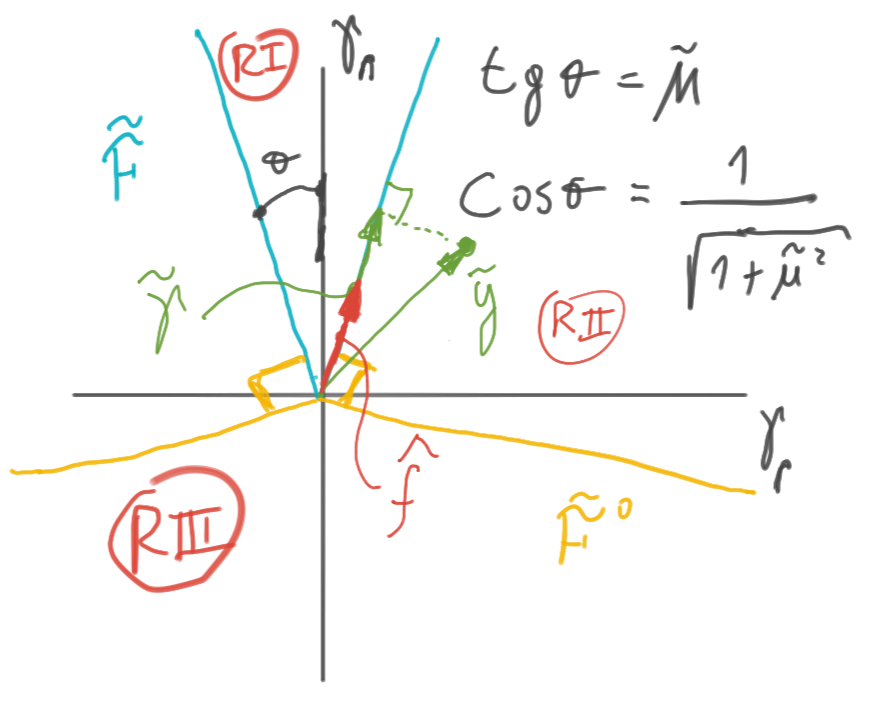
\includegraphics[width=0.45\columnwidth]{figures/cone_regions.png}
    \caption{Geometry of $\mathcal{F}_{\tilde\mu}$ and regions in the
    $\tilde{\vf{y}}$ space.}
    \label{fig:cone_regions}
\end{figure}

Finally, we obtain Eq. (\ref{eq:y_projection}) by applying the transformation
$\bgamma=\mf{R}^{-1/2}\tilde\bgamma$ to recover the impulses projected onto the
friction cone ${\mathcal{F}}_{\mu}$ using the norm in $\vf{R}$.

Though the tangent vector $\hat{\vf{t}}$ is not defined for $\vf{y}=\vf{0}$, the
projection still is, $P_\mathcal{F}(\vf{0})=\vf{0}$. In practice however, we
introduce a smooth \emph{soft-norm} defined as
$\|\vf{x}\|_s=\sqrt{\|\vf{x}\|^2+\varepsilon_s^2}$ and we define the tangent
vector as $\hat{\vf{t}}=\vf{y}_t/\Vert\vf{y}_t\Vert_s$. This newly defined tangent vector is smooth and has the desired property that it leads to the right
projection result in the limit to $\vf{y}\rightarrow 0$. In addition, not only
the projection is well defined, but also its gradients in Appendix
\ref{app:gradients_derivation}. In practice we use $\varepsilon_s=10^{-8}$.


\section{An Unconstrained Convex Formulation}
\label{sec:unconstrained_convex_formulation}

A remarkable property of the dual optimal solution, the impulses, is that they
can be can be constructed analytically from the optimal velocities of the primal
formulation in \eqref{eq:primal_regularized}. This is referred to as the
\textit{inverse dynamics} solution \cite{bib:todorov2014}. Moreover, given the
separable structure of the constraints, the impulse $\bgamma_i$ at the
$i\text{-th}$ contact point is the solution to the following convex optimization
problem
\begin{eqnarray}
	\bgamma_i(\vf{v}_{c,i})&=& P_{\mathcal{F}_i}(\vf{y}_i(\vf{v}_{c,i}))
	\nonumber\\
	&=&\begin{aligned} \argmin_{\bgamma\in\mathcal{F}_i} \quad &
		\frac{1}{2}(\bgamma-\vf{y}_i)^T\vf{R}_i(\bgamma-\vf{y}_i) \end{aligned}
	\label{eq:y_projection}\\
	\vf{y}_i(\vf{v}_{c,i}) &=& -\vf{R}_i^{-1}(\vf{v}_{c,i}-\hat{\vf{v}}_{c,i})	
\end{eqnarray}
where $\vf{R}_i\in\mathbb{R}^{3\times3}$ is the $k\text{-th}$ diagonal block of
the regularization matrix $\mf{R}$. That is, $\bgamma_i$ is the projection
$P_{\mathcal{F}_i}$ of $\vf{y}_i(\vf{v}_{c,i})$ onto the friction cone
$\mathcal{F}_i$ using the norm defined by $\vf{R}_i$.

We use the analytical inverse dynamics to write an unconstrained convex
formulation in terms of velocities only
\begin{eqnarray}
	\min_{\mf{v}} \ell_p(\mf{v}) = \frac{1}{2}\Vert\mf{v}-\mf{v}^*\Vert_{A}^2 +
	\frac{1}{2}\Vert P_\mathcal{F}(\mf{y}(\mf{v}))\Vert_R^2
	\label{eq:primal_unconstrained}
\end{eqnarray}
where, as with other quantities, we form $\mf{y}$ by stacking each
$\vf{y}_i$ from all contact pairs together. Given the separable structure of the
constraints, projection $P_{\mathcal{F}}(\mf{y})$ onto $\mathcal{F} :=
\mathcal{F}_1 \times F_2 \times \cdots \times \mathcal{F}_{n_c}$ in the norm
defined by $\mf{R}$ is formed by stacking together the individual projections
$P_{\mathcal{F}_i}(\vf{y}_i)$ from Eq. (\ref{eq:y_projection}).

The unconstrained formulation in Eq. (\ref{eq:primal_unconstrained}) includes
the same cost in velocities as the primal formulation from Eq.
(\ref{eq:primal_regularized}). However, the conic constraint $\mf{g}\in
\mathcal{F}^*$ in Eq. (\ref{eq:primal_regularized}) has been replaced by a cost
term using the analytical inverse dynamics. Lemma
\RedHighlight{Add proper reference} in Appendix \RedHighlight{Add proper reference} proofs
that the unconstrained cost $\ell_p(\mf{v})$ is strongly convex and
differentiable with Lipschitz continuous gradients. Therefore the problem
stated in Eq. (\ref{eq:primal_unconstrained}) has a unique solution.

We state the main result of this section in the following result, proved in
Appendix \ref{app:unconstrained_formulation_equivalance}.
\begin{theorem}
    The pair $\{\mf{v},\bsigma\}$, with velocities $\mf{v}$ solution to the
    unconstrained formulation in Eq. (\ref{eq:primal_unconstrained}) and
    $\bsigma=P_\mathcal{F}(\mf{y}(\mf{v}))$, is primal optimal of the primal
    formulation in Eq. (\ref{eq:primal_regularized}).
    \label{th:unconstrained_formulation_equivalance}
\end{theorem}

Section \ref{sec:sap_solver} presents our novel SAP solver specifically designed
to solve the unconstrained formulation in Eq. (\ref{eq:primal_unconstrained}).

% Dummy commit so that this file shows in Reviewable.

\algblockdefx{RepeatUntil}{EndRepeatUntil}{\textbf{repeat until}}{}
\algnotext{EndRepeatUntil}

\section{Semi-Analytical Primal Solver}
\label{sec:sap_solver}

SAP essentially is Newton's method
applied to the unconstrained formulation stated in
Eq. (\ref{eq:primal_unconstrained}), where constraints have been eliminated
using our analytical inverse dynamics. At the $m\text{-th}$ Newton iteration,
SAP uses analytical expressions of both the gradient and Hessian of
$\ell_p(\mf{v})$, along with a line search to find the unique optimal solution.
We use the previous time step velocity $\mf{v}_0$ to initialize the
iteration. The stopping criteria is discussed below in Section
\ref{sec:stopping_criteria}.

\begin{algorithm}[H]
	\caption{SAP Newton Iteration}	
	\label{alg:sap}
	\begin{algorithmic}[1]
		\State Initialize $\mf{v}^0 \gets \mf{v}_0$
		\RepeatUntil $~\Vert\tilde{\nabla}\ell_p\Vert < \varepsilon_a + \varepsilon_r\max(\Vert\tilde{\mf{p}}\Vert,\Vert\tilde{\mf{j}_c}\Vert)$, Eq. \eqref{eq:stopping_criteria}
			\State $\Delta\mf{v}^{m} = -\mf{H}^{-1}(\mf{v}^m)\nabla_\mf{v}\ell_p(\mf{v}^m)$ \label{op:Newton_iteration}
			\State $\displaystyle \alpha^m = \argmin_{t\in\mathbb{R}^{++}} \ell_p(\mf{v}^m + t \Delta\mf{v}^{m})$
			\State $\displaystyle \mf{v}^{m+1} = \vf{v}^m + \alpha^{m}\Delta\mf{v}^{m}$
		\EndRepeatUntil
		\State\Return $\{\mf{v}$, $\bgamma=P_\mathcal{F}(\vf{y}(\mf{v}))\}$
	\end{algorithmic}
\end{algorithm}

Specifics of the line search algorithm are critical to the success of the SAP
solver given that the cost can undergo large changes as $\mf{v}^m$ explores
states corresponding to different contact modes. We explore two line-search
algorithms: an approximate backtracking line-search with Armijo's stopping
criteria and an exact (to machine epsilon) line-search. We show how a careful
pre-computation of commonly occurring terms enables the exact line-search step
at a small fraction of the total cost. Though both line-search approaches
guarantee the convergence of SAP \RedHighlight{ref to Frank's proof}, we find
that the exact line-search can lead to a performance improvement between 15\% to
35\%. In the next subsections, we describe each component of the solver in
detail.

\subsection{Gradients}
\label{sec:gradients}

%Appendix \ref{app:gradients_derivation}

We summarize the main results required for implementation. The gradient of the
primal cost $\ell_p$ is
\begin{equation*}
	\nabla_\mf{v}\ell_p(\mf{v}) = \mf{A}(\mf{v}-\mf{v}^*) + \nabla_\mf{v}\ell_R,
\end{equation*}
where we define the regularizer cost as $\ell_R(\mf{v})=\frac{1}{2}\Vert
P_\mathcal{F}(\mf{y}(\mf{v}))\Vert_R^2$. We show in Appendix
\ref{app:gradients_derivation} that this gradient can be computed analytically as
\begin{equation}
	\nabla_\mf{v}\ell_p(\mf{v}) = \mf{A}(\mf{v}-\mf{v}^*) - \mf{J}^T\bgamma(\mf{v})
	\label{eq:primal_gradient}
\end{equation}
with $\bgamma(\mf{v})=P_\mathcal{F}(\vf{y})$ from the analytical inverse
dynamics in Eq. \eqref{eq:analytical_y_projection}. This recovers the original
momentum balance in Eq. (\ref{eq:momentum_linearized}) since Newton's method
solves for $\nabla_\mf{v}\ell_p=\mf{0}$.

We obtain the Hessian of the regularizer $\ell_R(\mf{v})$ from the
gradients of $\bgamma(\mf{v})$ as
\begin{eqnarray}
	\nabla_\mf{v}^2\ell_R(\mf{v}) &=& \mf{J}^T\mf{G}\,\mf{J}\nonumber\\
	\mf{G} &=&-\nabla_{\mf{v}_c}\bgamma = \nabla_\mf{y}\bgamma \mf{R}^{-1}
	\label{eq:ellR_hessian}
\end{eqnarray}
where $\nabla_{\mf{v}_c}\!\bgamma$ is a block diagonal matrix where each
diagonal block is the $3\times 3$ matrix $\nabla_{\mf{v}_{c,i}}\!\bgamma_i$
for the $i\text{-th}$ contact. As shown in Appendix
\ref{app:gradients_derivation}, $\nabla_{\mf{v}_c}\bgamma\succeq 0$ and thus
$\nabla_\mf{v}^2\ell_R(\mf{v})\succeq 0$.

Finally, the Hessian needed in Newton's method is
\begin{equation}
	\mf{H}= \mf{A} + \mf{J}^T\mf{G}\,\mf{J}
	\label{eq:ell_hessian}
\end{equation}
which, since $\mf{A}\succ 0$, is strictly positive definite. Notice
that to compute the required gradient and Hessian, we need analytical expressions
for the projection $P_\mathcal{F}(\vf{y})$ and its gradient
$\nabla_\mf{y}P_\mathcal{F}(\vf{y})$. They are provided in Appendices
\ref{app:analytical_inverse_dynamics_derivations} and
\ref{app:gradients_derivation} respectively.

\subsection{Line Search}

At the $m\text{-th}$ Newton iteration, backtracking line-search starts with a
maximum step length of $\alpha_\text{Max}$ and progressively decreases it
by a factor $\rho \in (0, 1)$ as $\alpha\gets\rho\alpha$ until Armijo's
criteria \cite[\S 3.1]{bib:nocedal2006numerical} is satisfied. We write Armijo's
criteria as $~\ell_p(\mf{v}^m + \alpha \Delta\mf{v}^{m}) < \ell_p(\mf{v}^m) +
c\,\alpha\,d\ell_p/d\alpha(\mf{v}^m)$. Typical parameters we use are
$\rho=0.8$, $c=10^{-4}$ and $\alpha_\text{Max}=1.5$.

Since the cost $\ell_p(\mf{v})$ is strongly convex and differentiable with
Lipschitz continuous gradients, see Lemma \RedHighlight{reference to Frank's
proof}, its restriction to a line $\ell(\alpha)$ inherits the following
properties
\begin{enumerate}
	\item $\ell_p(\alpha)$ is strictly convex, i.e. there is a unique minimum.
	\item Newton steps are well formed since $d^2\ell_p/d\alpha^2>0$.
	\item $\ell_p(\alpha)$ is a piecewise $C^1$ function. In other words,
	$d\ell_p/d\alpha$ is continuous but $d^2\ell_p/d\alpha^2$ might not be.	
	\item Given the regularization used to model friction and stiff compliance,
	gradients of $\ell_p(\alpha)$ can undergo large changes, even within a
	region where $\ell_p(\alpha)$ is continuous.
\end{enumerate}

This leads us to choose a one-dimensional strategy that is robust under these
conditions. We find the method \verb;rtsafe; in \cite[\S
9.4]{bib:numerical_recipes} to work the best. \verb;rtsafe; is a one-dimensional
root finder that uses the Newton-Raphson method and switches to bisection
whenever Newton's method leads to an iterate outside a search bracket or
whenever its convergence is slow. Using analytical first and second derivatives,
our line search simply reduces to finding the unique root of $d\ell/d\alpha$
using the \verb;rtsafe; algorithm. The high performance of this method allows us 
to iterate $\alpha$ to machine precision at a negligible impact on the
computational cost. In practice, this is our preferred algorithm since it allows
us to use very tight regularization parameters without having to tune line search parameters. Moreover, we observe 15\%-35\% performance improvement when
compared to the backtracking line-search.

\subsection{Efficient Analytical Derivatives For Line Search}

\verb;rtsafe; requires the first and second derivatives of $\ell_p$, while the
backtracking method only requires the first derivative to verify Armijo's
stopping criteria. We show how to compute these gradients efficiently in
$\mathcal{O}(n)$ operations.

Defining $\ell(\alpha) = \ell_p(\mf{v}+\alpha\Delta\mf{v})$, we can compute first
and second derivatives with respect to $\alpha$ using the gradient and Hessian
\begin{eqnarray}
	\frac{d\ell}{d\alpha}&=&\Delta\mf{v}^T\nabla_\mf{v}\ell(\alpha)\nonumber\\
	\frac{d^2\ell}{d\alpha^2}&=&\Delta\mf{v}^T\nabla_\mf{v}^2\ell(\alpha)\Delta\mf{v}\nonumber
\end{eqnarray}

These derivatives are expensive to compute for general non-linear functions, and
most line search variations in practice are approximations that avoid their
computation altogether. We show that first and second derivatives can be
computed efficiently given the structure of the problem.

Using the gradients from Section \ref{sec:gradients}, we can write
\begin{eqnarray}
	\frac{d\ell_M}{d\alpha}(\alpha)&=&\Delta\mf{v}^T\mf{A}(\mf{v}(\alpha)-\mf{v}^*)\\
	\frac{d\ell_R}{d\alpha}(\alpha)&=&-\Delta\mf{v}^T\mf{J}^T\bgamma.
\end{eqnarray}
Defining the change of constraint velocity
$\Delta\mf{v}_c=\mf{J}\Delta\mf{v}$ and change of momentum $\Delta\mf{p} =
\mf{A}\Delta\mf{v}$, we obtain the much simpler and faster to compute versions
\begin{eqnarray}
	\frac{d\ell_M}{d\alpha}(\alpha)&=&\Delta\mf{p}^T(\mf{v}(\alpha)-\mf{v}^*)\\
	\frac{d\ell_R}{d\alpha}(\alpha)&=&-\Delta\mf{v}_c^T\bgamma(\alpha)
\end{eqnarray}
which only require dot products that can be computed in $\mathcal{O}(n_v)$ and
$\mathcal{O}(n_c)$ respectively.

Using the same definitions, we can write simple expressions for the second
derivatives as well
\begin{eqnarray}
	\frac{d^2\ell_M}{d\alpha^2}(\alpha)&=&\Delta\mf{v}^T\mf{A}\Delta\mf{v}=\Delta\mf{v}^T\Delta\mf{p}\\
	\frac{d^2\ell_R}{d\alpha^2}(\alpha)&=&-\Delta\mf{v}_c^T
	\nabla_{\mf{v}_c}\bgamma\Delta\mf{v}_c.
\end{eqnarray}
Notice that $\frac{d^2\ell_M}{d\alpha^2}$ is independent of $\alpha$ and
can be precomputed before the line search, and
$\frac{d^2\ell_R}{d\alpha^2}$ only involves $\mathcal{O}(n_c)$ operations given
the block diagonal structure of $\nabla_{\mf{v}_c}\bgamma$.

\subsection{Problem Sparsity}
\label{sec:problem_sparsity}

The Hessian in Eq. (\ref{eq:ell_hessian}) inherits a block sparse structure from
the specific contact configuration of the problem. We seek to exploit this
structure when solving Line~\ref{op:Newton_iteration} at each iteration of Algorithm \ref{alg:sap}.
To that end, we use a supernodal Cholesky factorization \cite[\S
9]{bib:davis2016survey}. Implementing this factorization requires construction
of a \emph{junction tree}.  For this we apply the algorithm in
\cite{bib:smail2017junction}, using cliques of $\mf{J}\mf{J}^T$ as input. We
use the implementation from the Conex solver \cite{bib:permenter2020}.

The block sparsity of the Hessian is best described with an example. We organize
our multibody systems as a collection of articulated \emph{tree structures}, or
a \emph{forest}. Consider the system in Fig. \ref{fig:sparsity_example}.
\begin{figure}[!h]
	\centering
	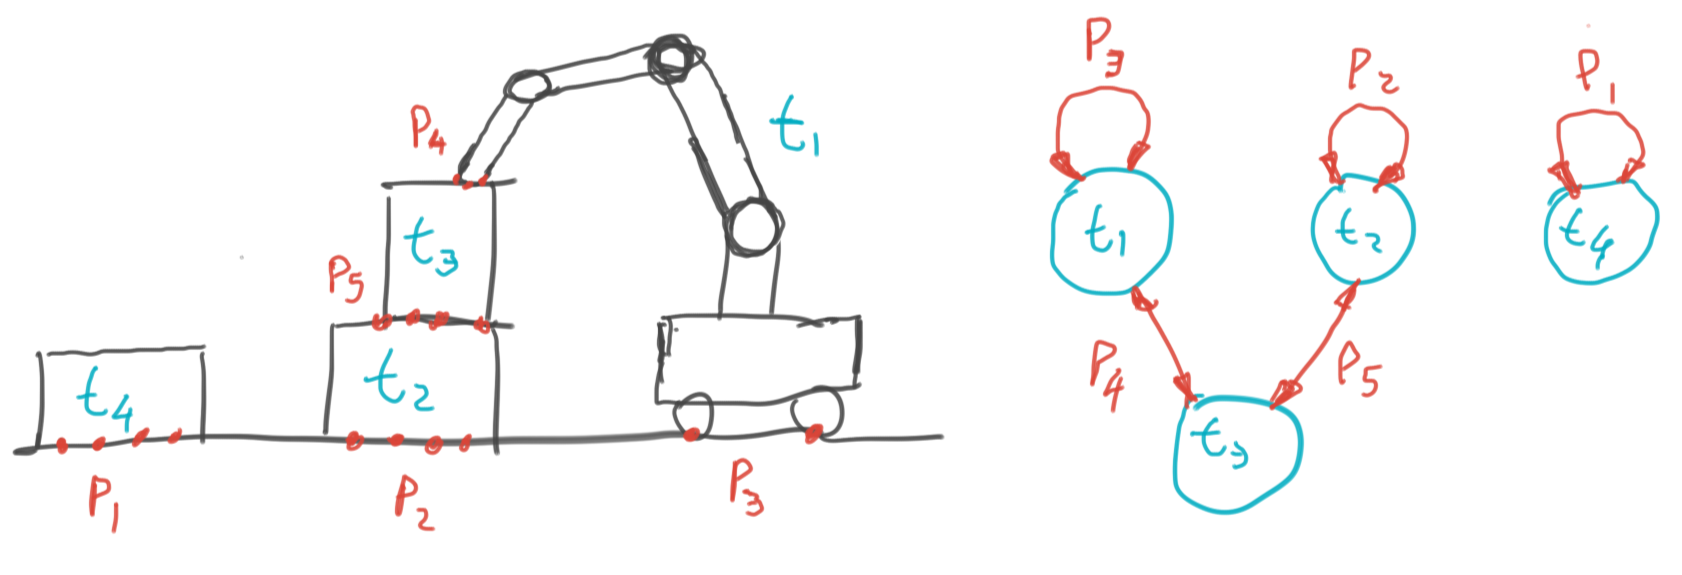
\includegraphics[width=0.7\columnwidth]{figures/sparsity_example.png}
	\caption{\label{fig:sparsity_example} 
	An example of a sparsity pattern commonly encountered in the
	simulation of robotic mechanical systems. The graph on the right puts
	\textit{trees} as nodes and contact \textit{patches} as edges. Notice how
	this graph exactly describes the sparsity pattern of the matrix
	$\mf{J}^T\mf{G}\mf{J}$ in Fig. \ref{fig:JTGJ_schematic}.}
\end{figure}
In this example, a robot arm mounted on a mobile base constitutes its own tree,
here labeled $t_1$. The number of degrees of freedom of the $t\text{-th}$ tree
will be denoted with $n_t$. A free body is the common case of a tree with
$n_t=6$. In general, the mass matrix will have a
block diagonal structure where the $t\text{-th}$ diagonal block corresponds to
the mass matrix of the $t\text{-th}$ tree. For the example in Fig.
(\ref{fig:sparsity_example}), the mass matrix looks like\\\\\\
\begin{equation}
	\mf{M}=\quad
	\begin{bmatrix}
		\tikzmark{M_topleft}
		\diagentry{\mf{M}_{\cc{11}}}&&&\tikzmark{M_topright}\\
		&\diagentry{\mf{M}_{\cc{22}}}\\
		&&\diagentry{\mf{M}_{\cc{33}}}\\		
		\tikzmark{M_bottomleft}&&&\diagentry{\mf{M}_{\cc{44}}}
	\end{bmatrix}
% Draw lil arrows on top and to the left.
\tikz[overlay,remember picture] {
	\draw[->,thick,color=cyan]
  ([yshift=3ex]M_topleft) -- ([yshift=3ex]M_topright) node[midway,above]
  {\scriptsize $t$}; 
  \draw[->,thick,color=cyan]
  ([yshift=1.5ex,xshift=-2ex]M_topleft) -- ([xshift=-4ex]M_bottomleft)
  node[near end,left] {\scriptsize $t$};}	
\end{equation}
\RedHighlight{Make this equation a Figure instead.}

We define as \textit{patches} a collection of contact pairs between two
trees. We label in red all contact patches in Fig. (\ref{fig:sparsity_example}).
Each contact pair corresponds to a single cone constraint in our
formulation. The set of constraint indexes that belong to patch $p$ is
denoted with $\mathcal{I}_p$ of size (cardinality) $|\mathcal{I}_p| = r_p$.

Notice that our definition of \textit{patches} is used to describe sparsity and
has nothing to do with the actual geometrical topology of the contact surface
between two trees. That is, the \textit{patches} could in
general correspond to either a single connected surface or a complex contact area
formed by a set of disconnected surfaces. Figure (\ref{fig:sparsity_example})
labels trees and patches and shows the corresponding graph where the nodes are
the trees and the edges are the contact patches.

Recall from Eq. (\ref{eq:ellR_hessian}) that $\mf{G} =
-\nabla_{\mf{v}_c}\bgamma$ is a block diagonal matrix, with $\vf{G}_i =
\nabla_{\vf{v}_{c,i}}\bgamma_i \in \mathbb{R}^{3\times 3}$ at the $i\text{-th}$
diagonal block. We can also write this as $\mf{G} = \text{diag}(\mf{G}_p)$ if we
group contact pairs by patches to define $\mf{G}_p=\text{diag}(\vf{G}_i),
\,\forall i\in\mathcal{I}_p$.

The contact Jacobian is in general sparse since the relative velocity at a
contact pair $i$ only involves the generalized velocities of the two trees
in contact. For the case in Fig. (\ref{fig:sparsity_example}), the Jacobian looks
like\\\\
\begin{equation}
	\mf{J}=\quad
	\begin{bmatrix}
		\tikzmark{J_topleft}\mf{0} & 
		\mf{0} & \mf{0} & \mf{J}_{\rr{1}\cc{4}}\tikzmark{J_topright}\\		
		\mf{0} & \mf{J}_{\rr{2}\cc{2}} & \mf{0} & \mf{0}\\
		\mf{J}_{\rr{3}\cc{1}} & \mf{0} & \mf{0} & \mf{0}\\
		\mf{J}_{\rr{4}\cc{1}} & \mf{0} & \mf{J}_{\rr{4}\cc{3}} & \mf{0}\\
		\tikzmark{J_bottomleft}
		\mf{0} & \mf{J}_{\rr{5}\cc{2}} & \mf{J}_{\rr{5}\cc{3}} & \mf{0}		
	\end{bmatrix}
% Draw lil arrows on top and to the left.
\tikz[overlay,remember picture] {
	\draw[->,thick,color=cyan]
  ([yshift=3ex]J_topleft) -- ([yshift=3ex]J_topright) node[midway,above]
  {\scriptsize $t$}; 
  \draw[->,thick,color=red]
  ([yshift=1.5ex,xshift=-3ex]J_topleft) -- ([xshift=-3ex]J_bottomleft)
  node[near end,left] {\scriptsize $p$};}	
\end{equation}
\RedHighlight{Make this equation a Figure instead.}\\
where each non-zero block is the Jacobian $\mf{J}_{\rr{p}\cc{t}}$ of size
$3r_p\times n_t$.

We have now the elements to describe the sparsity of the product
$\mf{J}^T\mf{G}\mf{J}$. For the example in Fig. \ref{fig:sparsity_example}, the
block sparsity of $\mf{J}^T\mf{G}\mf{J}$ is illustrated in Fig.
\ref{fig:JTGJ_schematic}. Notice how the sparsity pattern of
$\mf{J}^T\mf{G}\mf{J}$ exactly matches the graph from Fig.
(\ref{fig:sparsity_example}). Finally, the Hessian has the sparsity
structure of $\mf{A} + \mf{J}^T\mf{G}\mf{J}$.
\begin{figure*}[!h]
	\centering
	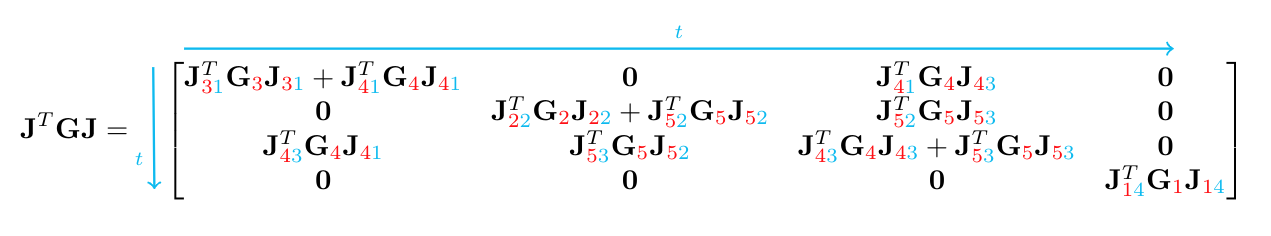
\includegraphics[width=0.8\textwidth]{figures/JTGJ_schematic.png}
	\caption{\label{fig:JTGJ_schematic} 
	Block sparsity of the $\mf{J}^T\mf{G}\mf{J}$ for the example illustrated in
	Fig. \ref{fig:sparsity_example}.}
\end{figure*}

Our implementation organizes the blocks of the Jacobian $\mf{J}$ as described in
this section, i.e. we condense rows by patches and columns by trees, so that the
supernodal Cholesky factorization can exploit this rich structure. Using this
block structure, the supernodal solver can take full advantage of specific
optimizations for dense algebra.



\subsection{Stopping Criteria}
\label{sec:stopping_criteria}

To assess convergence, we monitor the optimality condition for the unconstrained
problem in Eq. (\ref{eq:primal_unconstrained}) by evaluating the norm of the
momentum balance in Eq. (\ref{eq:primal_gradient})
\begin{equation}
	\nabla\ell_p(\mf{v}) = \mf{A}(\mf{v}-\mf{v}^*) - \mf{J}^T\bgamma.
\end{equation}

Notice that the components of $\nabla\ell_p$ have units of generalized momentum
$\mf{p}=\mf{M}\mf{v}$. Depending on the choice of generalized coordinates, the
generalized momentum components may have different units. In order to weigh all
components equally, we define the diagonal matrix $\mf{D} =
\text{diag}(\mf{M})^{-1/2}$ and perform the following change of variables
\begin{align}
	\tilde{\nabla}\ell_p &= \mf{D}\nabla\ell_p, \nonumber\\
	\tilde{\mf{p}} &= \mf{D}\mf{p}, \nonumber \\
	\tilde{\mf{j}}_c &= \mf{D}\mf{j}_c,
	\label{eq:scaled_momentum_quantities}
\end{align}
where we define the generalized contact impulse $\mf{j}_c=\mf{J}^T\bgamma$.
With this scaling, all the new \emph{tilde} variables have the same units,
square root of Joules. Using these definitions, we write our stopping criteria
as
\begin{equation}
	\Vert\tilde{\nabla}\ell_p\Vert < \varepsilon_a + \varepsilon_r\max(\Vert\tilde{\mf{p}}\Vert,\Vert\tilde{\mf{j}_c}\Vert).
	\label{eq:stopping_criteria}
\end{equation}
where $\varepsilon_r$ is a dimensionless relative tolerance that we usually set
in the range from $10^{-6}$ to $10^{-3}$. The absolute tolerance $\varepsilon_a$
is used to detect rare cases where the solution leads to no contact and no
motion, typically due to external forces. We always set this tolerance to a
small number, $\varepsilon_a=10^{-16}$.

\section{Test Cases}
\label{sec:test_cases}

We evaluate the robustness, accuracy, and performance of our method in a number
of simulation tests. All simulations are carried out in a system with 24 2.2
GHz Intel Xeon cores (E5-2650 v4) and 128 GB of RAM, running Linux. For all
solvers below however, all tests are run in a single thread.

For all of our simulations, unless otherwise specified, our model uses
$\beta=1.0$ and $\sigma=10^{-3}$ for the regularization parameters in Eq. (\ref{eq:normal_regularization}) and Eq. (\ref{eq:slip_time_scale}), respectively.

For SAP, tolerances for the stopping criteria are set to
$\varepsilon_a=10^{-16}$ and $\varepsilon_r=10^{-5}$. While the other solvers we use below use different stopping criteria, we use the same performance and accuracy metrics for all of them in order to perform a fair comparison.

\subsection{Performance Comparisons Against Other Solvers}
We evaluate commercial software Gurobi and Mosek to solve our convex
formulation of contact. Both solvers can solve a large variety of optimization
problems and are considered the industry standard. However, Mosek is not robust
for these problems and does not always find a solution. Therefore, we only present
comparison results with Gurobi.

As an open source option, we evaluate the Geodesic interior-point methods (IPM)
from \cite{bib:permenter2020}. Geodesic IPMs, in contrast with primal-dual
IPMs, do not apply Newton's method to the central-path conditions directly.
Instead, they use geodesic curves that satisfy the complementarity slackness
condition. This method has proven to warm start effectively when applied to
Model Predictive Control Problems \cite{bib:permenter2020} and therefore we are
interested in evaluating its performance for solving our convex formulation of
contact. Moreover, we use the Geodesic IPM solver's supernodal algebra described
in Section \ref{sec:problem_sparsity} in our implementation of SAP. Using the
same algebra for SAP and Geodesic IPM allows us to perform a fair comparison between
the two solvers; performance differences can be attributed to the properties
inherent to the optimization method instead of the differences in the linear
algebra operations.

\subsection{Spring-Cylinder}
\label{sec:spring_cylinder}
We model the setup shown in Fig. \ref{fig:spring_cylinder}, consisting
of a cylinder of radius $R=0.05\text{ m}$ and mass $m=0.5\text{ kg}$ connected
to a wall to its left by a spring of stiffness $k_s=100\text{ N}/\text{m}$.
While the cylinder is free to rotate and translate in the plane, the contact
force between the cylinder and the ground constrains the cylinder's motion in
the vertical direction. The contact stiffness is $k=10^{4}\text{ N}/\text{m}$
and the dissipation time scale is $\tau_d=0.02\text{ s}$. The cylinder is
initially placed with zero velocity at $x_0=0.1\text{ m}$ to the right of the
spring's resting position, and it is then set free.
\begin{figure}[!h]
	\centering
	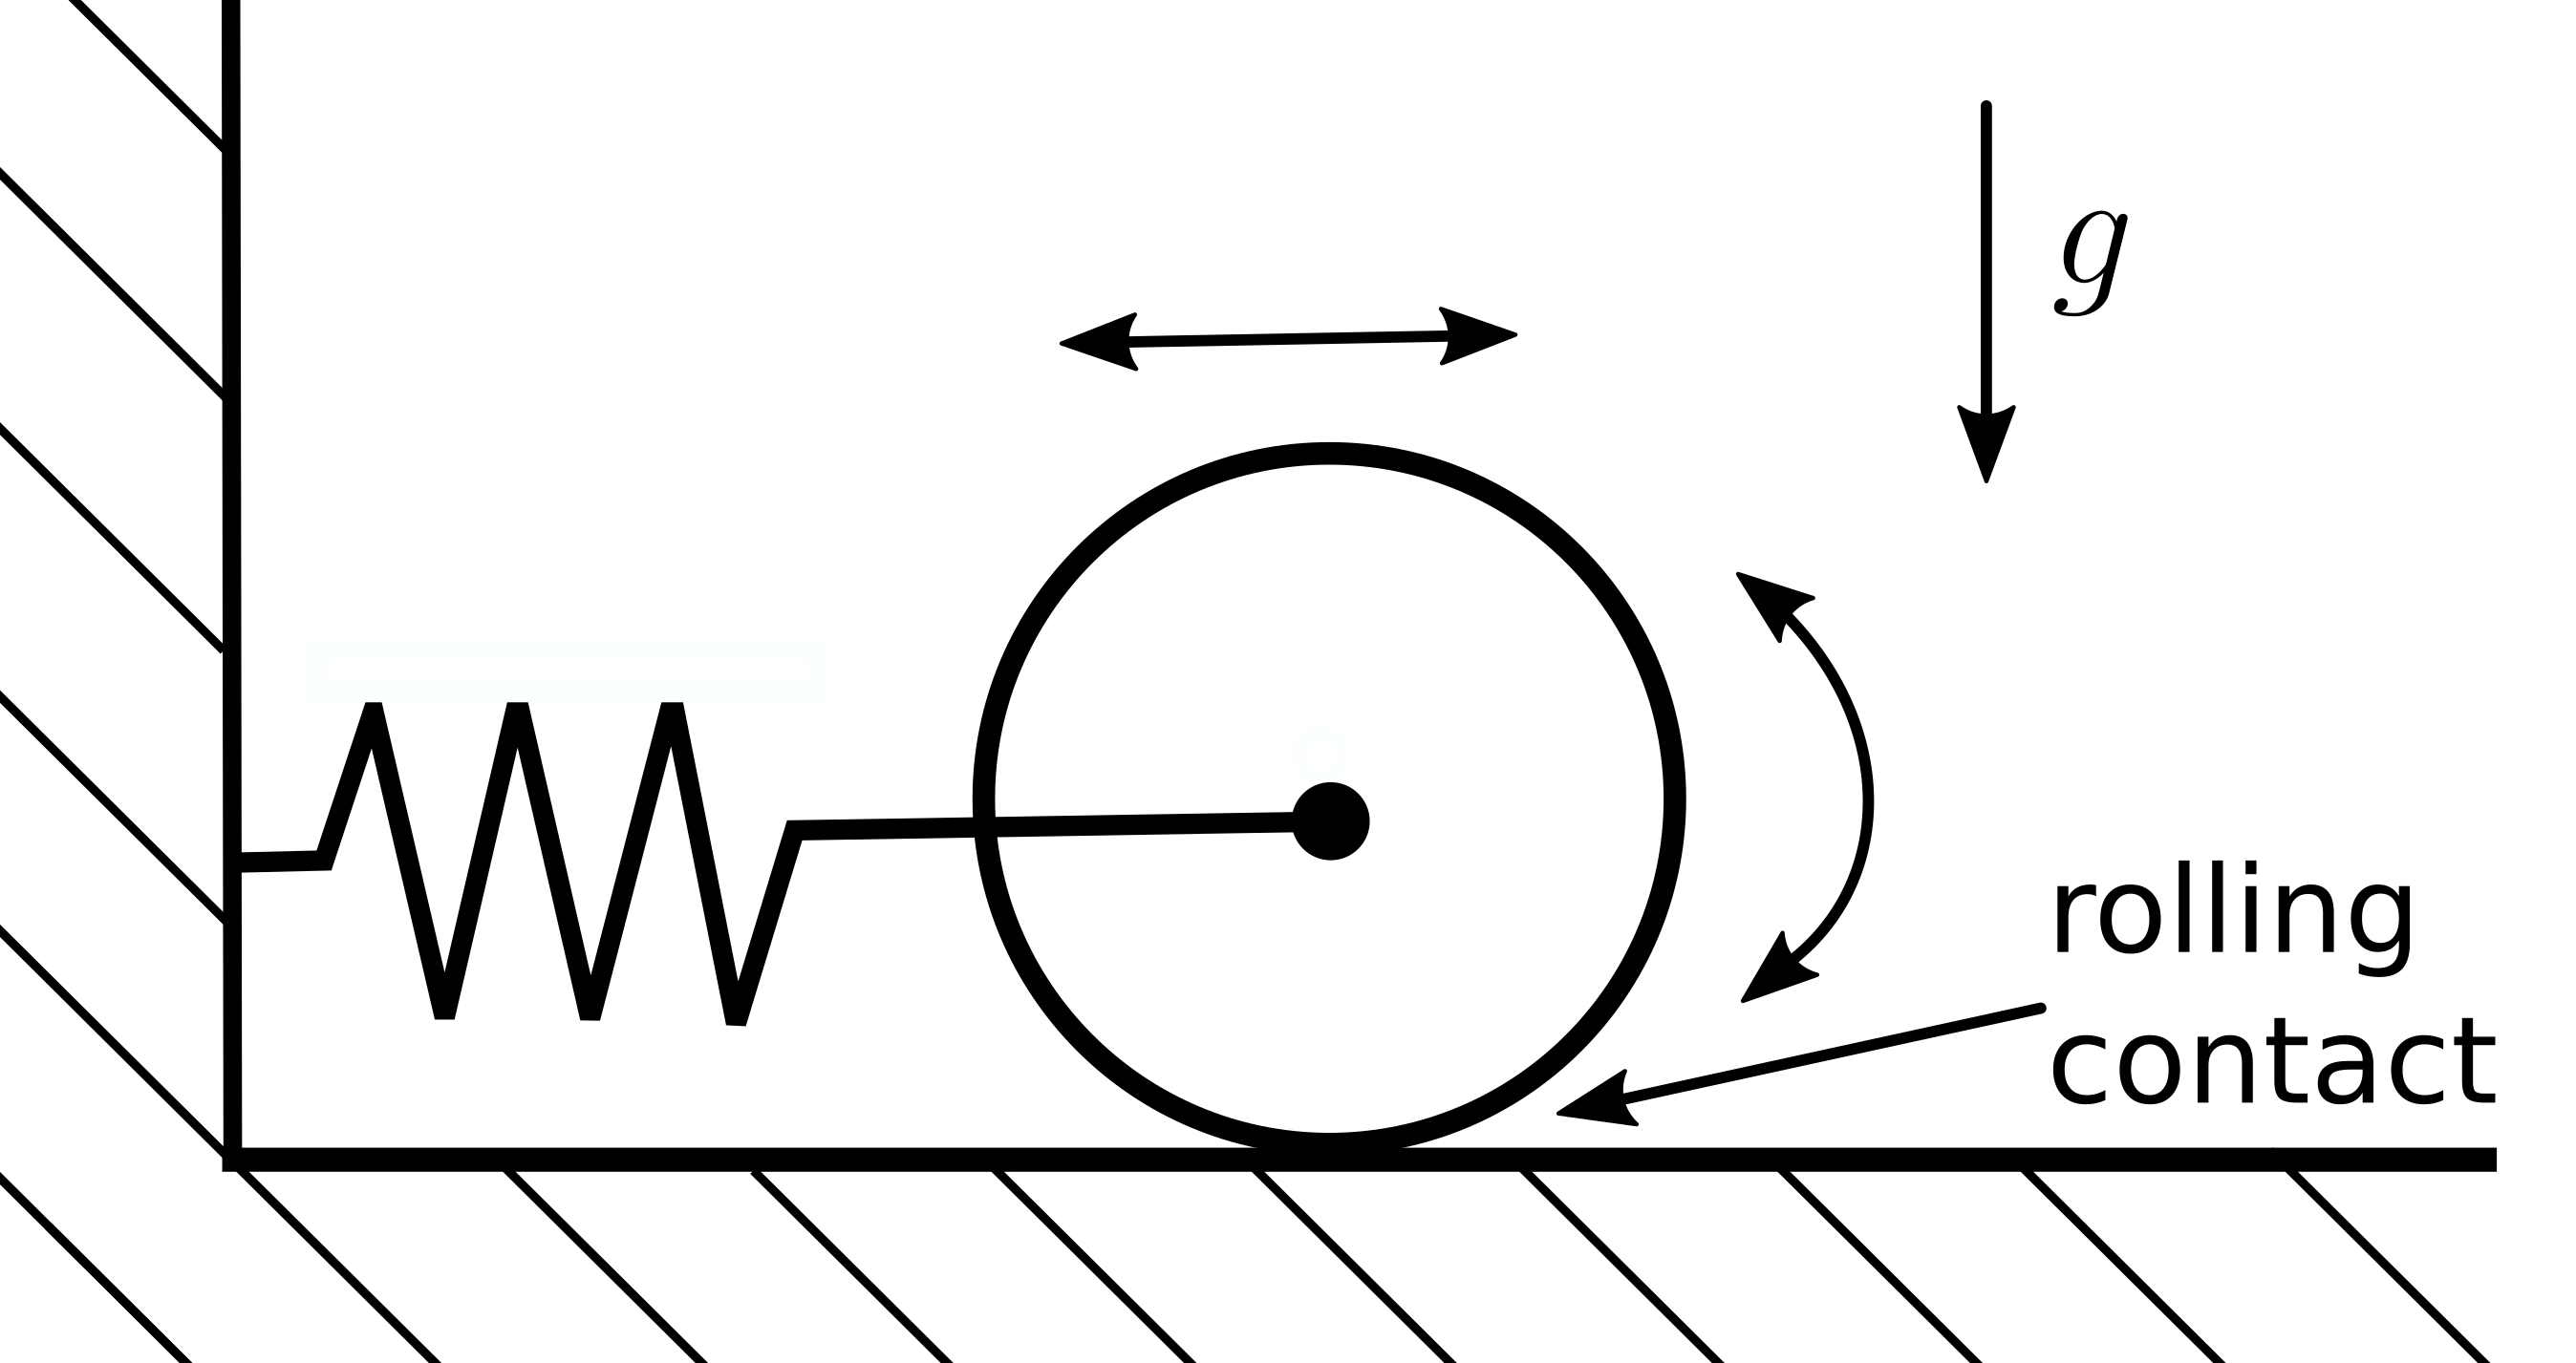
\includegraphics[width=0.6\columnwidth]{figures/schematics/spring_cylinder.png}
	\caption{\label{fig:spring_cylinder} 
	Spring-Cylinder system. The cylinder can translate horizontally and rotate.
	Friction with the ground establishes a non-dissipative rolling contact.}
\end{figure}

For reference, we first simulate this setup with frictionless contact, i.e.
$\mu=0$. Without friction, the cylinder does not rotate and we effectively have a
spring-mass system with natural frequency $\omega_n=\sqrt{k_s/m}$. We use a
rather coarse time step of $\delta t=0.02\text{ s}$, discretizing each period of
oscillation with about $22$ steps. Figure
\ref{fig:frictionless_spring_cylinder_energy} shows the total mechanical energy
as a function of time computed using three different schemes; symplectic Euler,
midpoint rule, and implicit Euler. The amount of numerical dissipation
introduced by the implicit Euler scheme dissipates the initial energy in just a
few periods of oscillation. For the symplectic Euler scheme, we observe in Fig.
\ref{fig:frictionless_spring_cylinder_energy} that, while the energy is not
conserved, it stays bounded, within a band 28\% peak-to-peak wide. The figure
also confirms that the second order midpoint scheme conserves energy exactly. These are well known theoretical properties of these
integration schemes when applied to the spring-mass system.
\begin{figure}[!h]
    \centering
    %trim={<left> <lower> <right> <upper>}
    \adjincludegraphics[width=0.49\columnwidth,trim={0 0 {0.05\width} 0},clip]{figures/spring_cylinder/frictionless_total_energy.png}
    \adjincludegraphics[width=0.49\columnwidth,trim={0 0 {0.05\width} 0},clip]{figures/spring_cylinder/frictionless_total_energy_long_term.png}    
    \caption{\label{fig:frictionless_spring_cylinder_energy} 
    Total mechanical energy for the frictionless spring-cylinder system in the
    first few periods of oscillation (left) and long term (right).}
\end{figure}

We now focus our attention to a case with frictional contact using $\mu=1$. As
we release the cylinder from its initial position at $x_0=0.1\text{ m}$,
friction with the ground establishes a rolling contact, and the system sets into
a periodic motion. Since now kinetic energy is split into translational and
rotational components, the rolling cylinder behaves as a spring-mass system with
an effective mass $m_\text{eff}=m+I_o/R^2$, with $I_o$ the rotational inertia of
the cylinder about its center. Therefore the frequency of oscillation is slower
and the same time step, $\delta t=0.02\text{ s}$, now discretizes one
period of oscillation with about 27 steps.

Total energy is shown in Fig. \ref{fig:spring_cylinder_energy}. Solutions computed with the implicit
Euler and the symplectic Euler schemes show similar trends to those in the frictionless
case. The midpoint rule does not conserve energy exactly, but it does
significantly better with a peak-to-peak variation of only 0.16\%. While the
ideal rolling contact does not dissipate energy, the regularized model of
friction does dissipate energy given the slip velocity is never exactly zero,
though small in the order of $\sim\sigma\mu\delta t g$ as shown in Section
\ref{sec:physical_intuition}. The symplectic Euler scheme and the midpoint rule
take $10$ minutes of simulated time and about $1000$ oscillations to dissipate
10\% of the total energy (Fig. \ref{fig:spring_cylinder_energy}, right). This
level of numerical dissipation is remarkably low, considering that real mechanical systems often introduce several sources of dissipation.
\begin{figure}[!h]
    \centering
    %trim={<left> <lower> <right> <upper>}
    \adjincludegraphics[width=0.49\columnwidth,trim={0 0 {0.05\width} 0},clip]{figures/spring_cylinder/total_energy.png}
    \adjincludegraphics[width=0.49\columnwidth,trim={0 0 {0.05\width} 0},clip]{figures/spring_cylinder/total_energy_long_term.png}    
    \caption{\label{fig:spring_cylinder_energy} 
    Total mechanical energy for the spring-cylinder system with friction $\mu=1$
    in the first few periods of oscillation (left) and long term (right).}
\end{figure}

To study the order of accuracy of our approach, we define the $L^2$-norm position error as
\begin{equation*}
    e_q = \left(\frac{1}{T}\int_0^T dt(x(t)-x_e(t))^2\right)^{1/2}
\end{equation*}
where $x_e(t)$ is the known exact solution. We simulate for $T=5\text{
s}$, about 10 periods of oscillation. Figure \ref{fig:spring_cylinder_position_error} shows the position error as
a function of the time step. We see that even with frictional contact, the two-stage approach
with the midpoint rule achieves second order of accuracy. Both the implicit Euler and the symplectic Euler schemes are first order,
though the error is significantly smaller when using the symplectic Euler
scheme.
\begin{figure}[!h]
	\centering
	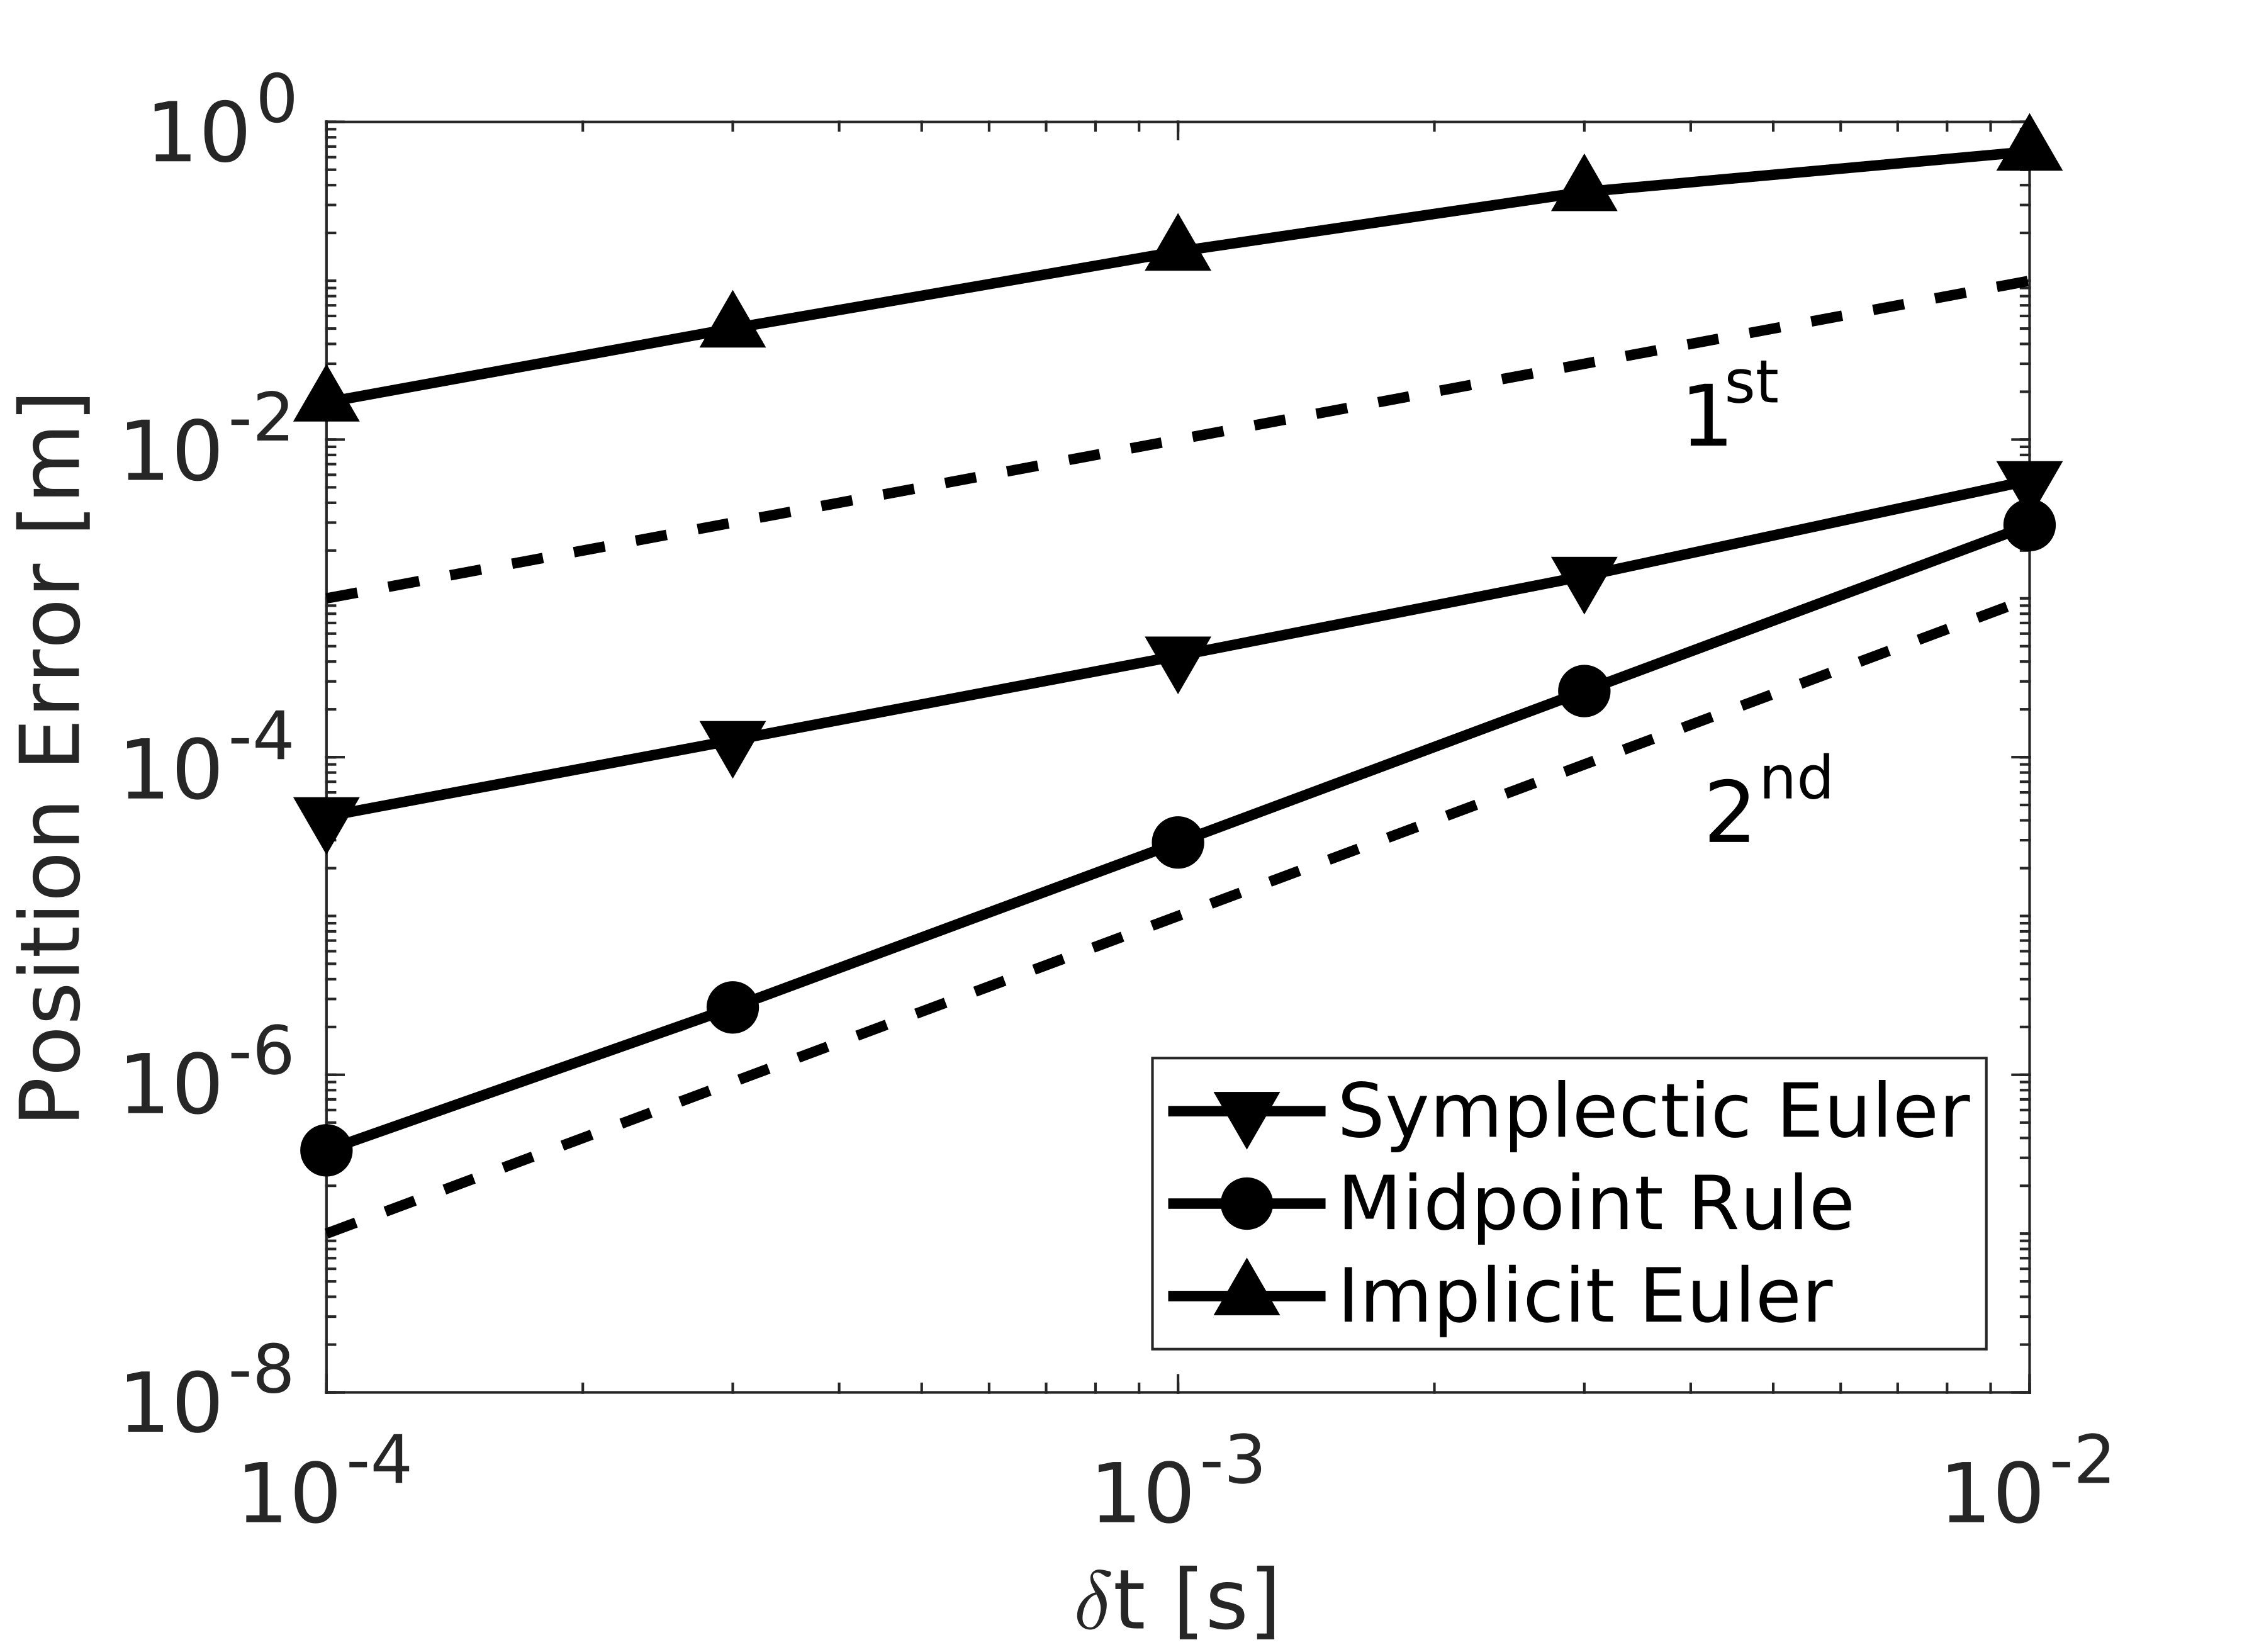
\includegraphics[width=0.7\columnwidth]{figures/spring_cylinder/position_error.png}
	\caption{\label{fig:spring_cylinder_position_error} 
	Position error as a function of time step for the spring-cylinder system
	with friction. First and second order references are shown with dashed
	lines.}
\end{figure}

\subsection{Clutter}
\label{sec:clutter}

The purpose of this case is to evaluate robustness, convergence properties, and
scalability of our SAP solver when compared against other existing methods.

The setup consists of an open container with a square base of size
$80~\text{cm}\times80~\text{cm}$ and $80~\text{cm}$ in height. Bodies are
dropped into this container in four different columns with the same number of
bodies each (see Fig. \ref{fig:clutter_snapshots}). Each column consists of an
arbitrary assortment of spheres of radius $5~\text{cm}$ and boxes with sides of
$10~\text{cm}$ in length. All bodies have density $1000\text{
kg}/\text{m}^3$ and therefore each sphere has a mass of approximately
$0.524\text{ kg}$ and each box has a mass of $1.0\text{ kg}$. We set a very high
contact stiffness of $k=10^{12}\text{ N}/\text{m}$ so that the model is in the
\emph{near-rigid} regime. The dissipation time scale is set to equal the time
step and the friction coefficient of all surfaces is $\mu=1.0$.
\begin{figure}[t]
    \centering
    %trim={<left> <lower> <right> <upper>}
    \adjincludegraphics[width=0.49\columnwidth,trim={0 {0.05\height} 0 0},clip]{figures/clutter/clutter_w_walls_t0.png}
    \adjincludegraphics[width=0.49\columnwidth,trim={0 {0.05\height} 0 0},clip]{figures/clutter/clutter_no_walls_t0.png}\\
    \vspace{0.1cm}
    \adjincludegraphics[width=0.49\columnwidth,trim={0 {0.05\height} 0 0},clip]{figures/clutter/clutter_w_walls_t2_zoom.png}
    \adjincludegraphics[width=0.49\columnwidth,trim={0 {0.05\height} 0 0},clip]{figures/clutter/clutter_no_walls_t2_zoom.png}
    \caption{Initial conditions (top) and an intermediate configuration after $2$ seconds of
    simulated time (bottom) for the clutter setup with (left) and without
    (right) walls. Many of the spheres in the configuration with no walls
	roll outside the frame in the intermediate configuration.}
    \label{fig:clutter_snapshots}
\end{figure}

We first run our simulations with 10 bodies per column for a total of 40 bodies.
We simulate 10 seconds using time steps of size $\delta t = 10\text{ ms}$.
Number of solver iterations and wall-clock time per time step are reported in
Fig. \ref{fig:clutter_w_walls_nb40} for the three solvers. We observe that SAP
needs to perform a larger number of iterations during the very energetic initial
transient. As the system reaches a steady state, however, SAP warm starts very
effectively, performing only about $3$ iterations per time step. Even though
SAP necessities a larger number of iterations to converge than Geodesic IPM during this initial transient, the wall-clock time per time step is very
similar. This tells us that SAP's cost per iteration is lower than that of
Geodesic IPM, even when they both use the same supernodal algebra. Unlike SAP and Geodesic IPM that benefit from warm start, we see that Gurobi performs
about $9$ iterations per time step in both the initial transient and the steady state.

\RedHighlight{TODO: Don't forget to add a plot showing convergence. Probably for
a worst case taking about 25 iterations and for a mean case taking about 5
iterations.}

\begin{figure}[!h]
	\centering
    %trim={<left> <lower> <right> <upper>}
    \adjincludegraphics[width=0.49\columnwidth,trim={0 0 {0.05\width} 0},clip]{figures/clutter/iterations_nb40.png}
    \adjincludegraphics[width=0.49\columnwidth,trim={0 0 {0.05\width} 0},clip]{figures/clutter/wall_clock_nb40.png}    
	\caption{\label{fig:clutter_w_walls_nb40} 
	Iterations and wall-clock time per time step for SAP, Geodesic IPM, and
	Gurobi for the clutter case with 40 bodies and with walls. Most of the
	energy is lost during the first $\sim300$ time steps as the objects pile up
	at the bottom of the box.}
\end{figure}

\subsubsection{Scalability}

We evaluate the performance of SAP with different problem sizes by varying the
number of objects in the clutter with all other parameters held constant. We
study scalability of the test case both with and without walls (see
Fig. \ref{fig:clutter_snapshots}) as the variation in the setup leads to very
different sequences of contact configuration. The size of the problems can be
appreciated in Fig. \ref{fig:clutter_num_contats} showing the number of contact
constraints at the end of the simulation when objects are in steady state
against the number of objects. We observe a larger number of contacts for the
configuration without walls since in this configuration many of the boxes spread
over the ground and lay flat on one of their faces, leading to a multi-contact
configuration (see Fig. \ref{fig:clutter_snapshots} for instance). Notice that
each body contributes 6 DOFs and each contact constraint contributes 3 unknowns.
Therefore, in the case with 200 bodies, the problem involves 1200 DOFs and about
2700 contact unknowns for a total of about 3000 unknowns.
\begin{figure}[!h]
	\centering
	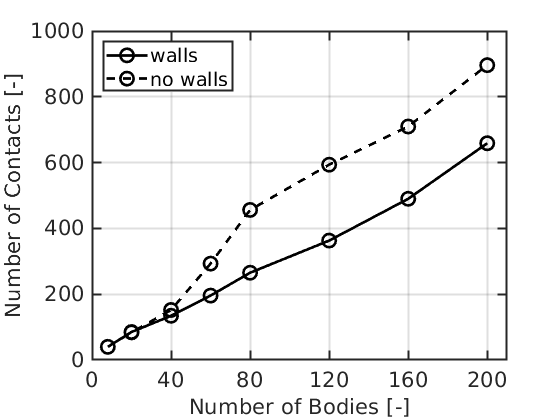
\includegraphics[width=0.6\columnwidth]{figures/clutter/number_of_contacts.png}
	\caption{\label{fig:clutter_num_contats} 
	Total number of contacts with objects in steady state at the end of the
	simulation for setup with and without walls.}
\end{figure}

We measure the total time spent by each solver and define the \emph{speedup}
against Gurobi. Figure \ref{fig:clutter_speedup} shows the speedup for both
SAP and Geodesic IPM in the configuration with and without walls.
The setup with walls is particularly difficult given that objects are
constrained to pile up, leading to a configuration in which almost all objects
are coupled with every other object by frictional contact
(see Fig. \ref{fig:clutter_snapshots}). That is, the motion of an object at the
bottom of the pile can lead to motion of another object far on top of the pile.
In contrast, the simulation with no walls leads to \emph{islands} of objects
that do not interact with each other.

In general, we observe two regimes. For problems with less than about 40 bodies,
SAP outperforms Gurobi significantly by up to a factor of 25 in the case with
walls and up to a factor of 50 with no walls. Beyond 80 bodies, Gurobi
outperforms both SAP and Geodesic IPM in the case with walls, but SAP is about
10 times faster for the case with no walls. Though SAP shows to be about twice
as fast as Geodesic IPM for most problem sizes, it can be five times faster for
small problems with 8 bodies or less.
\begin{figure}[!h]
	\centering
    %trim={<left> <lower> <right> <upper>}
    \adjincludegraphics[width=0.49\columnwidth,trim={{0.02\width} 0 {0.05\width} 0},clip]{figures/clutter/speedup_w_walls.png}
    \adjincludegraphics[width=0.49\columnwidth,trim={{0.02\width} 0 {0.05\width} 0},clip]{figures/clutter/speedup_no_walls.png}
	\caption{\label{fig:clutter_speedup} 
	Speedup against Gurobi for both SAP and Geodesic IPM for the configuration with walls (left) and without walls (right).}
\end{figure}

It could be argued that these speedup results depend on the accuracy settings of
each solver. For a fair comparison, we define the dimensionless momentum error
as
\begin{equation}
	e_m = \frac{\Vert\tilde{\nabla}\ell_p\Vert}{\max(\Vert\tilde{\mf{p}}\Vert,\Vert\tilde{\mf{j}_c}\Vert)},\nonumber
\end{equation}
using the scaled generalized momentum quantities in Eq.
(\ref{eq:scaled_momentum_quantities}). We assess the accuracy of the
complementarity slackness with the dimensionless quantity
\begin{eqnarray*}
	e_\mu = \frac{1/n_c\sum_i|\bm{g}_i\cdot\bgamma_i|}{\ell_p}.
\end{eqnarray*}

Figure \ref{fig:clutter_errors_w_wall} shows average values of $e_m$ and $e_\mu$
over all time steps. Since SAP satisfies the complementarity slackness exactly,
$e_\mu$ is not shown. We have verified this to be true within machine precision
for all simulated cases.

SAP's momentum error is below $10^{-5}$ as expected since this is the value used
for the termination condition. Similarly, the complementarity slackness is below
$10^{-5}$ for Geodesic IPM, since this is the value used for its own termination
condition. Gurobi does a good job at satisfying the complementarity slackness.
However, it is the solver with the largest error in the momentum equations, even
though both SAP and Geodesic IPM outperform Gurobi in most of the test cases.
These metrics demonstrate that when SAP and Geodesic IPM outperform Gurobi, it
is not at the cost of losing accuracy.
\begin{figure}[!h]
	\centering
    %trim={<left> <lower> <right> <upper>}
    \adjincludegraphics[height=0.40\columnwidth,trim={0 0 {0.05\width} 0},clip]{figures/clutter/momentum_error_w_walls.png}
	\adjincludegraphics[height=0.40\columnwidth,trim={{0.05\width} 0 {0.05\width} 0},clip]{figures/clutter/momentum_error_no_walls.png}\\
    \adjincludegraphics[height=0.40\columnwidth,trim={0 0 {0.05\width} 0},clip]{figures/clutter/optimality_condition_error_w_walls.png}
    \adjincludegraphics[height=0.40\columnwidth,trim={{0.05\width} 0 {0.05\width} 0},clip]{figures/clutter/optimality_condition_error_no_walls.png}
	\caption{\label{fig:clutter_errors_w_wall} 
	Momentum balance error $e_m$ (top) and complementarity condition error
	$e_\mu$ (bottom) for the clutter case with walls (left) and without walls
	(right).}
\end{figure}

\subsubsection{Slip Parameter}

We study the effect of the slip parameter $\sigma$ in Eq.
(\ref{eq:slip_time_scale}). As before, we use $\delta t = 10\text{ ms}$ and
simulate 40 objects for 10 seconds to a steady state configuration. At this
steady state at the end of the simulation, we compute the mean slip velocity
among all contacts. Figure \ref{fig:clutter_sigma_vt} shows this mean slip
velocity along with the estimated slip in Eq. (\ref{eq:slip_estimation}), $v_s
\approx\sigma\mu\delta t g$, shown in dashed lines. We see that the mean slip
velocity remains below the estimated slip as expected in a static configuration
with objects in stiction. In the case with walls where stiction helps to hold
the steady state static configuration, we see that the mean slip velocity
closely follows the slope of the slip estimate. Without the walls, objects do
not pile up in a complex static structure but simply lie on the ground, and
therefore, the resulting slip velocities are significantly smaller. The sudden
drop in the slip velocity for $\sigma>10^{-3}$ is caused by the sensitivity of
the final state on the value of $\sigma$. As $\sigma$ increases, so does the
slip velocity bound $v_s$ and objects in the configuration without walls can
slowly drift into a configuration leading to more contacts. In particular, boxes
are more likely to slowly drift until one of their faces lies flat
on the ground, a configuration with zero slip once steady state is reached.
Finally, we observe that when using $\sigma=10^{-3}$, the amount of slip is
negligible for robotic applications.
\begin{figure}[!h]
	\centering
	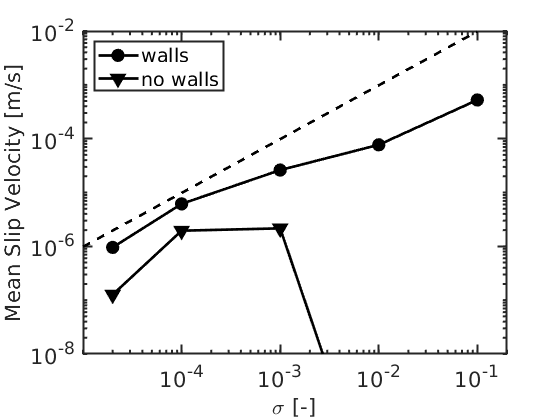
\includegraphics[width=0.6\columnwidth]{figures/clutter/sigma_vt.png}
	\caption{\label{fig:clutter_sigma_vt} 
	Mean slip velocity at the end of the simulation with objects at rest as a
	function of the slip parameter. The estimated slip $v_s = \sigma\mu\delta t g$ is shown in dashed lines.}
\end{figure}

We conclude by examining the effect of $\sigma$ on the conditioning of the
system. Figure \ref{fig:clutter_sigma} shows the condition number of the Hessian
in the final configuration and the mean number of Newton iterations throughout
the simulation. We see that the condition number scales as $\sigma^{-1}$ while
the mean number of Newton iterations is roughly proportional to  $\ln(\sigma)$.
Notice that our choice $\sigma=10^{-3}$ for this paper is placed right in the
middle, in a log scale, of the range of values examined in this study.
\begin{figure}[!h]
	\centering
    %trim={<left> <lower> <right> <upper>}
    \adjincludegraphics[width=0.49\columnwidth,trim={0 0 {0.05\width} 0},clip]{figures/clutter/sigma_iterations.png}
    \adjincludegraphics[width=0.49\columnwidth,trim={0 0 {0.05\width} 0},clip]{figures/clutter/sigma_condition_number.png}
	\caption{\label{fig:clutter_sigma} 
	Effect of the slip parameter on the conditioning of the system. Mean Newton iterations per step (left) and mean condition number (right).}
\end{figure}

    
\section{Constraints Based Modeling Framework}
\label{sec:constraints_based_modeling_framework}

This extends the work in \cite{bib:todorov2014} by using regularization to model
true physical compliance instead of a means to introduce a Baumgarte-style
stabilization. As a result, we not only obtain a model that enables the modeling
of true compliant elements, but we gain a very simple to understand insight on
the unphysical artifacts introduced by the convex approximation of contact.

We consider holonomic constraints $\mf{p}(\mf{q};t)=\mf{0}$ as well as
non-holonomic constraints $\mf{u}(\mf{v}; \mf{q},t)=\mf{J}_u\,\mf{v}+\mf{b}_u=
\mf{0}$. We treat both sets of constraints at the velocity level to write
\begin{equation}
	\mf{v}_c = \mf{J}\mf{v}+\mf{b}=\mf{0}
	\label{eq:velocity_level_constraints}
\end{equation}
where $\mf{v}_c$ is the constraints velocity, $\mf{J}$ the constraints Jacobian
and $\mf{b}$ is a velocity bias.

In our compliant formulation of constraints we relax Eq.
(\ref{eq:velocity_level_constraints}) so that when impulses $\bgamma$ are in the
interior of $\mathcal{C}$, they behave as the linear spring and damper law
\begin{equation}
	\bgamma = -dt(\mf{k}\,\mf{p} + \mf{c}\,\mf{v}_c)
	\label{eq:compliant_constraints}
\end{equation}
where stiffness $\mf{k}$ and damping $\mf{c}$ matrices are diagonal. For
Non-holonomic constraints stiffness is zero and damping \textit{regularizes} the
problem.

In the discrete time setting we again use the $\theta\text{-method}$ with
parameter $\theta_c$, different from $\theta$ in Eq.
(\ref{eq:v_update}) to gain more control on the stability and
accuracy of the method. E.g.: we typically use $\theta_c=1$ for contact
constraints for additional stability while we use $\theta_c=1/2$ for holonomic
constraints for better energy conservation. Using $\mf{v}_c^{\theta_c}$ and
$\mf{p}^{\theta_c}=\mf{p}_0+dt\mf{v}_c^{\theta_c}$ in Eq.
(\ref{eq:compliant_constraints}) and grouping terms we can write

\begin{eqnarray}
	\gamma_i &=& -R_i^{-1}(v_{c,i}-\hat{v}_i)\nonumber\\
	R_i^{-1} &=& \theta_c dt (dt\,k_i+c_i)\nonumber\\
	\hat{v}_i &=& -\frac{k_i}{\theta_c(dt\,k_i+c_i)}p_{0,i}-
	              \frac{1-\theta_c}{\theta_c}v_{c0,i}
\end{eqnarray}
\todo{contrast this to Torodorv's stabilization and show how his is unstable.}

We can then define the regularization matrix $\mf{R}=\text{diag}(\{R_i\})$ and
fit the compliant laws within the framework developed in \cite{bib:todorov2014}
\begin{eqnarray}
	\mf{y} &=& -\vf{R}^{-1}(\mf{v}_c-\hat{\mf{v}}) \label{eq:y_definition}\\
	\bgamma &=& P_\mathcal{C}(\mf{y})
	\label{eq:projection_definition}
\end{eqnarray}
where $P_\mathcal{C}(\mf{y})$ is the projection onto $\mathcal{C}$ of $\mf{y}$
using the norm defined by $\vf{R}$. That is
\begin{equation}
	\begin{aligned}
		P_\mathcal{C}(\mf{y})=\argmin_{\bgamma\in\mathcal{C}} \quad & \frac{1}{2}(\bgamma-\mf{y})^T\mf{R}(\bgamma-\mf{y})
	\end{aligned}
\end{equation}

That is, while the impulse is strictly inside the convex set $\mathcal{C}$, Eq.
(\ref{eq:y_definition}) essentially enforces a penalty on the constraint
violation untilt $\mf{y}$ comes out of $\mathcal{C}$ and then Eq.
(\ref{eq:projection_definition}) projects it back to its boundary.

Before jumping into the details provided in Section
\ref{app:analytical_inverse_dynamics_derivations} here we'll summarize how, with
the proper definition of the velocity bias $\hat{\mf{v}}$, convex set
$\mathcal{C}$ and regularization $\mf{R}$, we can model a variety of physical
effects such as
\begin{itemize}
	\item Joint limits.
	\item Joint dry friction.
	\item PD control with force limits.
	\item Frictional contact.
\end{itemize}
\todo{continue propagating $\theta_c$ to the rest of the constraints.}

\subsection{Joint Limits}

Given a one-dof joint modeled with (scalar) minimal coordinates $q$ and $v$, we
can model the limit $q_l < q < q_u $ using two constraints (one for each, lower
and upper). In this case we have
\begin{eqnarray}
	\mf{g} &=&
	% J*v
	\begin{bmatrix}
		v\\
		v\\
	\end{bmatrix} -
	% vhat
	\begin{bmatrix}
		\hat{v}_l\\
		\hat{v}_u\\
	\end{bmatrix}\\
	\mf{R} &=& R\,\mf{I}_2
\end{eqnarray}
with
\begin{eqnarray}
	\hat{v}_l&=&-\frac{q_0-q_l}{\theta_c(dt+\tau)}-\frac{1-\theta_c}{\theta_c}v_0\\
	\hat{v}_u&=&-\frac{q_0-q_u}{\theta_c(dt+\tau)}-\frac{1-\theta_c}{\theta_c}v_0\\
	R^{-1}&=&\theta_c dt^2 k(1+\tau/dt)
\end{eqnarray}
where the dissipation rate $\tau$ is defined such that $c=\tau\,k$. The convex
set is $\mathcal{C}=\mathbb{R}^+$ with the projection
\begin{eqnarray}
	\gamma = y^+= \max(0, y)
\end{eqnarray}


\subsection{Joint Dry Friction}

In this case we'd like the joint impulse to be limited within an interval
$\mathcal{C} = [-dt\tau_M, dt\tau_M]$, where $\tau_M$ is a specified load.
Within that interval, given our regularized model, we'd like the joint force to
penalize motion. We can achieve this with
\begin{equation}
	y = -dt\frac{\tau_M}{v_s}v
\end{equation}

where $v_s$ is a \textit{stiction tolerance} with units of m/s for prismatic
joints and with units of rad/s for revolute joints. Therefore we have
\begin{eqnarray}
	\hat{v} &=& 0\nonumber\\
	R^{-1} &=& dt\frac{\tau_M}{v_s}
\end{eqnarray}

\subsection{PD Control with Force Limits}
In this case stiffness and dissipation are replaced by proportional and
derivative PD gains, respectively. To make the analogy with a spring-mass model
closer, the proportional gain is written as $k_p = k$ and the derivative gain as
$k_d = c = \tau k_p$. For this case $\mathcal{C} = [\gamma_l, \gamma_u] =
[dt\,u_l, dt\,u_u]$, where $u_l < u_u$ are lower and upper actuation limits.  In
this case, when inside the set $\mathcal{C}$, we want the impulse to be
\begin{eqnarray}
	y/dt = -k_p(q-q_d)-k_d(v-v_d)
\end{eqnarray}
where $q_d$ and $v_d$ are desired position and velocity respectively. We can
accomplish this with
\begin{eqnarray}
	\hat{v} &=& -\frac{q_0-q_d}{dt+\tau}+\frac{\tau}{dt}v_d\nonumber\\
	R^{-1}  &=& dt^2k(1+\tau/dt)
\end{eqnarray}

The convex set is $\mathcal{C} = [dt\,u_l, dt\,u_u]$ with projection
\begin{equation}
	\gamma = \min(\gamma_u, \max(\gamma_l, y))
\end{equation}


\subsection{Frictional Contact}
In this case we have
\begin{equation}
	\vf{g} = \vf{v}_c - \hat{\vf{v}}_c = \mf{J_c}\mf{v} - \hat{\vf{v}}_c
\end{equation}
where $\mf{J}_c$ is the contact Jacobian and 
\begin{eqnarray}
	\hat{\vf{v}}_c &=&
	\begin{bmatrix}
		0\\
		0\\
		\hat{v}_n \end{bmatrix}\nonumber\\
	\hat{v}_n &=& -\frac{\phi_0}{dt+\tau}\nonumber\\
	\mf{R} &=& \text{diag}([R_t, R_t, R_n]) = 
	\begin{bmatrix}
		R_t &   0 & 0\\
		  0 & R_t & 0\\
		  0 &   0 & R_n
	\end{bmatrix}
\end{eqnarray}
with $R_n^{-1} = dt^2k(1+\tau/dt)$ and $R_t=\sigma_t R_n$, where the
dimensionless parameter $\sigma_t$ allow us to control the amount of
regularization in the tangential direction.

In this case the convex set is the friction cone $\mathcal{C} = \mathcal{F}$ and
the projection can be computed in closed form as

\begin{equation}
	\bgamma = P_\mathcal{F}(\vf{y}) = 
\begin{dcases}
	% Region I, stiction
	\vf{y} 
	% When we  have:
	& \text{stiction, } y_r < \mu y_n\\
	%
	%
	% Region II, sliding.
	\begin{bmatrix}
		\mu\gamma_n\hat{\vf{t}}\\
		\frac{1}{1+\tilde\mu^2}\left(y_n +
	\mu\frac{R_t}{R_n}y_r\right)
	\end{bmatrix}
	% When we  have:
	& \text{sliding, } -\mu \frac{R_t}{R_n} y_r < y_n \leq \frac{y_r}{\mu}\\
	%
	%
	% Region III, no contact.
    \vf{0} & \text{no contact, } y_n \leq -\mu \frac{R_t}{R_n} y_r
\end{dcases}	  
	\label{eq:contact_projection}
\end{equation}
where $\vf{y}_t$ and $y_n$ are the tangential and normal components of $\vf{y}$,
the radial component is defined as $y_r=\Vert\vf{y}_t\Vert$ and the tangent
vector as $\hat{\vf{t}}=\vf{y}_t/y_r$. We also defined the common dimensionless
factors $\tilde\mu=\mu\,(R_t/R_n)^{1/2}$ and $\hat\mu=\mu\,R_t/R_n$.


\section{Physical Intuition, Principle of Maximum Dissipation and Artifacts}
\label{sec:physical_intuition}

\RedHighlight{you might probably start a subsection here on the physical
insight for these equations?}

To gain physical insight on what exaclty these forces are modeling, we
substitute $\vf{y}=\mf{R}^{-1}(\vf{v}_c - \hat{\vf{v}}_c)$ into Eq.
(\ref{eq:contact_projection}) to obtain an expression of the impulse as a
function of signed distance $\phi$ and normal and tangential velocities, $v_n$
and $\vf{v}_t$

\begin{eqnarray}
	&&\bgamma = P_\mathcal{F}(\vf{y}) = \\
&&\begin{dcases}
	% Region I, stiction
	\begin{bmatrix}
		-\vf{v}_t/R_t\\
		-dt(k\phi + c v_n)
	\end{bmatrix}
	% When we  have: y_r < \mu y_n
	& \text{stiction, } \\
	%
	%
	% Region II, sliding.
	\begin{bmatrix}
		\mu\gamma_n\hat{\vf{t}}\\
		-\frac{dt}{1+\tilde\mu^2}\left(k(\phi-(dt+\tau)\mu\Vert\vf{v}_t\Vert) + cv_n \right)
	\end{bmatrix}
	% When we  have:  -\mu \frac{R_t}{R_n} y_r < y_n \leq \frac{y_r}{\mu}
	& \text{sliding, }\\
	%
	%
	% Region III, no contact.  y_n \leq -\mu \frac{R_t}{R_n} y_r
    \vf{0} & \text{no contact, }
\end{dcases}\nonumber
	\label{eq:gamma_piecewise}
\end{eqnarray}
where $\phi= \phi_0 + dt\,v_n$.

From this expanded solution we see that friction forces behave exactly as a
model of regulirized friction
\begin{equation}
	\bgamma_t = -\min\left(\frac{\Vert\vf{v}_t\Vert}{R_t}, \mu\gamma_n\right)\hat{\vf{t}}
\end{equation}
That is, in the \textit{stiction} regime, regularized friction behaves as a high
viscosity fluid and it satisfies the maximum dissipation principle during
\textit{sliding}. This expression show us the convenience of having a separate
regularization coefficient $R_t$ for the tangential direction. It allows us to
control the stiction approximation separately from the compliance in the normal
direction introduced by $R_n$. To better model stiction we make the choice
$R_t=\sigma_t R_n$, with $\sigma_t \ll 1$, typically $\sigma_t=10^{-3}$ in our
simulations.

In the stiction region, we see that the normal forces model compliant contact
with linear stiffness $k$ and linear dissipation $c$. 

In the sliding region we see however that the convex approximation introduces
unphysical artifacts. Recall we are interested in the limit $R_t \ll R_n$ to
model better stiction and therefore $\tilde\mu \rightarrow 0$. This makes the
factor $1+\tilde{\mu}^2$ close to one and we can ignore it in our analysis.
While we'd like to recover $\gamma_n = -dt(k\phi + c v_n)$ as in stiction, we
instead see that the slip velocity $\Vert\vf{v}_t\Vert$ unphysically couples
into the normal forces as $\gamma_n=-dt(k(\phi-(dt+\tau)\mu\Vert\vf{v}_t\Vert) +
cv_n)$. 

This is consistent with the formulation in \cite{bib:anitescu2010} for rigid
contact when $k\rightarrow \infty$ leading to an unphysical \textit{gliding
effect} at a positive distance $\phi=dt\mu\Vert\vf{v}_t\Vert$. Notice that
\textit{gliding} goes away as $dt\rightarrow 0$ since the formulation converges
to the original contact problem \cite{bib:anitescu2006}. The effect of
compliance is to \textit{soften} this effect. 

In the limit to $dt\rightarrow 0$ we find out that the convex approximation
models, when sliding, the force law
$\gamma_n=-dt(k(\phi-\tau\mu\Vert\vf{v}_t\Vert)$. This tells us that, unlike the
rigid case, the \textit{gliding} effect unfortunately does not go away as
$dt\rightarrow 0$ but it persists with a finite value that now depends on the
dissipation rate, $\phi\approx\tau\mu\Vert\vf{v}_t\Vert$.

We close this discussion by making the following remarks relevant to robotics
applications:
\begin{enumerate}
	\item In robotics applications we are mostly interested in the stiction
	regime, typically for grasping, locomotion or rolling contact for mobile
	bases with wheels. This regime is precisely where the convex approximation
	does not introduce artifacts.
	\item Sliding is usually avoided or if importnat, it is usually at low
	velocities and therefore the term $dt\mu\Vert\vf{v}_t\Vert$ is negligible.
	\item Even though the effect of sliding cannot be neglected in the
	dissipation term during stiction, we point out that for robotics
	applications most often dissipation is high to model a zero restitution
	coefficient. Therefore the high dissipative nature of this term makes the
	effect of $\Vert\vf{v}_t\Vert$ negligible for most cases with low slip
	velocities.
	\item For robotics, we are definitely interested on the onset to sliding.
	This is captured by the approximation which properly models the Colulomb
	friction law.
\end{enumerate}

\section{Rigid Contact}
\todo{explain how Todorov's choice leads to an unstable time stepping schem while this scheme is unconditionally stable.}

Todorov in \cite{bib:todorov2014} sets the regularization parameters as
$R_i=\varepsilon N_{ii}$, where $\varepsilon$ is a small dimensionless
coefficient that controls the amount of regularization. Higher regularization
makes the problem better conditioned though at the expense of large compliance
and a poor stiction approximation. Lower regularization will converge to the
\textit{hard constraints} limit, however leading to a poorly conditioned
formulation. 

In this work we choose $\varepsilon$ from an analysis of the time scales
introduced by this regularization. The basic idea is that if the time scales
introduced by this numerical compliance cannot be resolved by a given time step
size $dt$, the system is effectively rigid. It essentially makes no difference
on the results if regularization is decreased beyond this point. 

For each contact point we define $g_i=\Vert\mathbf{W}_{ii}\Vert/3$ where
$\mathbf{W}_{ii}$ is the $3\times 3$ diagonal block of the Delassus operator
$\mathbf{W}$. The factor $3$ in our definition is so that $g_i$ is the RMS value
of the entries of $\mathbf{W}_{ii}$. This definition ensures that $g_i > 0$.
$g_i$ has unit of $\text{kg}^{-1}$ and represents the inverse of an effective
mass $m_i=g_i^{-1}$ for the $i\text{-th}$ contact. For instance, for the contact
between a point mass $m$ and the ground we have $g_i=(3m)^{-1}$ and $m_i=3m$,
see Section \ref{sec:conveyor_belt}. 

Regularization in the normal direction introduces a numerical compliance of
stiffness $k$, see Section \ref{sec:physical_intuition}, and this will therefore
induce a dynamics with a natural frequency in the order of $\omega_n^2=k/m_i$.
This relates to the period $T_n$ of this dynamics by $\omega_n=2\pi/T_n$.

Since the time stepping scheme will not resolve time scales in the order or
below the time step $dt$, we want to choose our regularization parameters so
that the numerical dynamics introduced cannot be resolved. We then make $T_n =
\alpha dt$, with alpha $\alpha \approx 1.0$. Therefore we need for the stiffness
$k=4\pi^2m_i/(\alpha^2 dt^2)$. We learned in Section
\ref{sec:physical_intuition} that $R_n=(dt^2\,k)^{-1}$ and therefore we arrive
to the final expression for our regularization in the normal direction
\begin{equation}
	R_n = \frac{\alpha^2}{4\pi^2}g_i = \frac{\alpha^2}{4\pi^2}\Vert\mathbf{W}_{ii}\Vert
\end{equation}

This is the same as Todorov's regularization taking $\varepsilon =
\alpha^2/(4\pi^2)\approx 0.025\,\alpha^2$. This analysis shows us that:
\begin{itemize}
	\item We can use a single parameter $\varepsilon$, independent of the time
	step, that leads to essentially the same numerically introduced artificial
	dynamics. 
	\item When $\alpha=1.0$ we have $\varepsilon=0.025$ which introduces a fair
	amount of regularization into the system. However the numerical time scales
	are only within $dt$ and are underresolved, as desired.
\end{itemize}

It is useful to estimate the amount of penetration for a point mass resting on
the ground. In this case we have
\begin{eqnarray}
	\phi &=& \frac{m\,g}{k} \nonumber\\
	&=& \frac{\alpha^2}{4\pi^2}\frac{m}{m_i}\,g\,dt^2\nonumber\\
	&=& \frac{\alpha^2}{12\pi^2}\,g\,dt^2
\end{eqnarray}

Taking $\alpha=1.0$ and on Earth's gravity, a typical simulation time step of
$dt=10^{-3}~\text{s}$ leads to $\phi\approx 8.3\times 10^{-8}~\text{m}$ and
using a very large simulation time tep of $dt=10^{-2}~\text{s}$ leads to
$\phi\approx 8.3\times 10^{-6}~\text{m}$, well within acceptable bounds for
typical robotics applications.

There is another reason to choose $\alpha\approx 1.0$. As we will see in the
example of Section \ref{sec:conveyor_belt}, the numerical dynamics is close to
being critically damped and numerical oscillations due to regularization are
damped out within a few time steps, independent of step size (see Fig.
\ref{fig:normal_velocity}). This is an expected result if we consider the
stability analysis on an implicit Euler scheme, which resembles this formulation
very closely when we think of it as an implicit scheme on a multibody system
with the compliant forces  in Section \ref{sec:physical_intuition}. This is a
very desired effect for us being interested on robotics applications with
perfectly inelastic contact.


\section{Conclusion}
\label{sec:future_directions}

We presented a formulation of compliant contact with a novel physics-based
parameterization. We showed that forces can be succinctly described by analytical
expressions with a clear physical intuition. This allowed us to incorporate not
only point contact but also more complex models of surface patches. We then showed
that when these forces are used in the momentum equations, we obtain the
optimality conditions for an unconstrained convex formulation. We made a
rigorous presentation of the numerical approximations and a novel
characterization of the artifacts introduced by the convex approximation of
contact; the approximation is exact for sticking contact and introduces an
$\mathcal{O}(\delta t\|\vf{v}_t\|)$ \emph{gliding} effect for sliding contact.

We developed a two-stage time stepping approach based on the
$\theta\text{-method}$ and we showed that with the midpoint rule it can achieve
second order accuracy even in problems with frictional contact. Our formulation
does not linearize the friction cone but it works with the second order cone
constraints directly.

We presented SAP, a robust and performant open source solver for this formulation that
warm-starts very effectively in practice. SAP 
globally convergences at least at a linear-rate and exhibits quadratic convergence when when additional smoothness conditions are satisfied. We showed that SAP
exhibits these two convergence regimes in simulations of practical relevance. We
provided thorough details for implementation, including analytical
formulae for gradients and Hessian, sparsity analysis and custom line-search.

We compared the performance of SAP against commercial and open source
optimization solvers. Using quantitative accuracy metrics we showed that SAP
outperforms the alternatives not only without sacrificing accuracy, but even at
higher accuracy and added robustness. SAP can be up to 50 times faster than
Gurobi in small problems with up to a dozen objects and up to 10 times faster in
medium sized problems with about 100 objects. Even though SAP uses the
supernodal algebra implemented for Geodesic IPM, it performs at least two times
faster due to its effective warm-starts from the previous time-step
solution. Moreover, SAP is significantly more robust in practice given
that it guarantees a hard bound on the error in momentum, effectively providing
a certificate of accuracy.

We have incorporated SAP into the open source robotics toolkit Drake
\cite{bib:drake}, and hope that the simulation and robotics communities can
benefit from our contribution.


\appendices
\section{Proof of Proposition \ref{prop:gradient_of_m_approximation}}
\label{app:gradient_of_m_approximation}
The Taylor expansion of $\mf{m}(\mf{v})$ at $\mf{v}=\mf{v}^*$ reads
\begin{align}
	\mf{m}(\mf{v}) &= \mf{m}^* + \frac{\partial \mf{m}}{\partial \mf{v}} (\mf{v}-\mf{v}^*) +
	\mathcal{O}_m(\Vert\mf{v}-\mf{v}^*\Vert^2)\nonumber\\
	&=\frac{\partial \mf{m}}{\partial \mf{v}}(\mf{v}-\mf{v}^*) +
	\mathcal{O}_m(\Vert\mf{v}-\mf{v}^*\Vert^2),
	\label{eq:m_taylor_expansion}
\end{align}
where we use the fact that by definition $\mf{m}^*=\mf{m}(\mf{v}^*)=\mf{0}$. All
derivatives are evaluated at $\mf{v} = \mf{v}^*$ unless otherwise noted. We
first evaluate the Jacobian of the mass matrix term in Eq.
(\ref{eq:m_definition})
\begin{align*}
	\frac{\partial \left( \mf{M}(\mf{q}^{\theta}(\mf{v}))(\mf{v}-\mf{v}_0) \right)}{\partial \mf{v}}
	= \mf{M}(\mf{q}^{\theta}(\mf{v}^*)) + \mf{E},
\end{align*}
where we defined
\begin{align*}
	\mf{E} = \frac{\partial \mf{M}(\mf{q}^{\theta})}{\partial\mf{v}} (\mf{v}^*-\mf{v}_0).
\end{align*}
Note that by combining Eqs. (\ref{eq:theta_method}) and (\ref{eq:scheme_q_update}), the
mid-step configuration $\mf{q}^{\theta}$ can be written as
\begin{align*}
	\mf{q}^{\theta}(\mf{v}) &= \mf{q}_0 + \delta t \theta \dot{\mf{q}}^{\theta_{vq}} \\
	                          &= \mf{q}_0 + \delta t \theta \mf{N}(\mf{q}^{\theta})\mf{v}^{\theta_{vq}}(\mf{v}).
\end{align*}
Hence by the chain rule, $\mf{E}$ can be further calculated as
\begin{align*}
	\mf{E} = \delta t\theta\frac{\partial \mf{M}(\mf{q}^{\theta}) }{\partial\mf{q}}
             \frac{\partial\dot{\mf{q}}^{\theta_{vq}}}{\partial\mf{v}}
			 (\mf{v}^*-\mf{v}_0).
\end{align*}
Notice that 
\begin{align*}
		\Vert\mf{E}\Vert 
		&\le \delta t\theta \left\| \frac{\partial\mf{M}(\mf{q}^{\theta})}{\partial\mf{q}}  \right\|
			\left\| \frac{\partial\dot{\mf{q}}^{\theta_{vq}}}{\partial\mf{v}}  \right\|
		    \left\| \mf{v}^*-\mf{v}_0 \right\| \\
		&= \mathcal{O}(\delta t^2),
\end{align*}
since $\Vert\mf{v}^*-\mf{v}_0\Vert = \mathcal{O}(\delta t)$.

We proceed similarly to expand the Jacobian of
$\mf{F}_1(\mf{v})=\mf{F}_1(\mf{q}^{\theta}(\mf{v}), \mf{v}^{\theta}(\mf{v}))$
as
\begin{align*}
	\frac{\partial\mf{F}_1}{\partial \mf{v}} = -\delta t\,\theta\theta_{vq}\mf{K}(\mf{q}^{\theta},
	\mf{v}^{\theta})-\theta\mf{D}(\mf{q}^{\theta}, \mf{v}^{\theta}),
\end{align*}
with $\mf{K}$ and $\mf{D}$ the stiffness and damping matrices defined by Eqs.
(\ref{eq:stiffness_matrix})-(\ref{eq:dissipation_matrix}).

We can now write the Jacobian of $\mf{m}(\mf{v})$ in Eq.
(\ref{eq:m_taylor_expansion}) as
\begin{align*}
	\frac{\partial \mf{m}}{\partial \mf{v}} = \mf{A} + \mf{E} - \delta t\frac{\partial \mf{F}_2}{\partial \mf{v}},
\end{align*}
where we defined
\begin{align*}
	\mf{A}=\mf{M}+ \delta t^2\theta\theta_{qv}\mf{K}+\delta t\theta\mf{D}.
\end{align*}
With these definitions the Taylor expansion in Eq. (\ref{eq:m_taylor_expansion})
becomes
\begin{align*}
	\frac{\partial\mf{m}}{\partial\mf{v}}(\mf{v}-\mf{v}^*) &= \mf{A}(\mf{v}-\mf{v}^*) + \mf{E}(\mf{v}-\mf{v}^*) \\
	&- \delta t\frac{\partial\mf{F}_2}{\partial\mf{v}}(\mf{v}-\mf{v}^*) + \mathcal{O}_m(\Vert\mf{v}-\mf{v}^*\Vert^2).
\end{align*}

Since contact is compliant, forces are finite within the finite interval $\delta
t$ and therefore $\Vert\mf{v}-\mf{v}^*\Vert=\mathcal{O}(\delta t)$. Thus
\begin{align*}
	\mf{E}(\mf{v}-\mf{v}^*)=\mathcal{O}_E(\delta t^3), \\
    \delta t\frac{\partial \mf{F}_2}{\partial \mf{v}}(\mf{v}-\mf{v}^*)=\mathcal{O}_{F_2}(\delta t^2), \\ 
    \mathcal{O}_m(\Vert\mf{v}-\mf{v}^*\Vert^2) = \mathcal{O}_m(\delta t^2).
\end{align*}
Therefore, the positive definite linearization
\begin{align*}
	\mf{A}(\mf{v}-\mf{v}^*) + \mathcal{O}_E(\delta t^3) + \mathcal{O}_{F_2}(\delta t^2) +
	\mathcal{O}_m(\delta t^2) = \mf{J}^T\mf{\bgamma},
\end{align*}
agrees with the original momentum balance in Eq. (\ref{eq:scheme_momentum}) to second
order.

Finally, notice that $\mf{A}$ is a linear combination of positive definite
matrices with non-negative scalars in the linear combination, and therefore
$\mf{A}\succ 0$.\hfill\IEEEQED


%\section{Proof of Theorem \ref{th:primal_dual}}
%\label{app:primal_dual_proof}
%The Lagrangian of the primal formulation in Eq. (\ref{eq:primal_regularized}) is
\begin{equation}
    \mathcal{L}(\mf{v},\bsigma,\vf{\gamma}) = 
\frac{1}{2}\Vert\mf{v}-\mf{v}^*\Vert_A^2 + \frac{1}{2} \Vert\bsigma\Vert_{R}^2 - \vf{\gamma}^T\mf{g}
    \label{eq:primal_lagrangian}
\end{equation}
with $\vf{\gamma}\in\mathcal{F}$ the dual variable to enforce the constraint
$\vf{g}\in \mathcal{F}^*$. Minimizing the Lagrangian in
\eqref{eq:primal_lagrangian} jointly in variables $\mf{v}$ and $\bsigma$ leads
to the optimality conditions
\begin{subequations}\label{eq:primal_optimality_conditions}
\begin{align}
    \mf{A}(\mf{v}-\mf{v}^*) &= \mf{J}^T\vf{\gamma} \label{eq:momentum_optimality}\\
    \vf{\sigma} &= \vf{\gamma}.  \label{eq:sigma_equal_gamma}
\end{align}
\end{subequations}
The optimality condition \eqref{eq:momentum_optimality} reveals that the
multipliers $\bgamma$ are indeed the contact impulses, and we recover the
balance of momentum. The optimality condition \eqref{eq:sigma_equal_gamma}
allows us to eliminate $\vf{\sigma}$. We then substitute these results back into
the Lagrangian in \eqref{eq:primal_lagrangian} to recover the dual in
\eqref{eq:dual_regularized}
\begin{align*}
    \min_{\bgamma\in \mathcal{F}} \ell_d(\bgamma) =
    \frac{1}{2}\bgamma^T(\mathbf{W}+\mathbf{R})\bgamma + {\bm r}^T
    \bgamma
\end{align*}
where, in contrast to previous work, our Delassus operator
$\mf{W}=\mf{J}\mf{A}^{-1}\mf{J}^T$ now also contains the contribution of
internal force elements (through Eq. (\ref{eq:expression_for_A})) and
$\mf{r}=\mf{v}_c^*-\hat{\mf{v}}_c$ with
$\mf{v}_c^*=\mf{J}\mf{v}^*$.\hfill\IEEEQED


\section{Proof of Theorem \ref{th:unconstrained_formulation_equivalance}}
\label{app:unconstrained_formulation_equivalance}
Before proving this theorem, we need the following result.
\begin{lemma}
    The conic constraint $\mf{g}(\mf{v}, \bsigma)\in\mathcal{F}^*$ is satisfied
    if $\bsigma$ is given by $P_\mathcal{F}(\mf{y(\mf{v})})$.
    \label{lemma:conic_constraints_are_satisfied_analytically}
\end{lemma}
\begin{IEEEproof}
    Since $\bsigma$ is the projection of $\mf{y}(\mf{v})$ to the cone
    $\mathcal{F}$ with the $\mf{R}$ norm, by Moreau's decomposition theorem, we
    know that $\mf{y}(\mf{v}) - \bsigma$ is in the polar cone of $\mathcal{F}$
    with the $\mf{R}$ norm. That is,
    \begin{align*}
        \langle \mf{y}(\mf{v}) - \bsigma, \mf{x} \rangle_\mf{R} \le 0 
    \end{align*}
    for all $\mf{x} \in \mathcal{F}$, with the inner product
    $\langle\mf{v},\mf{w}\rangle_\mf{R}=\mf{v}^T\mf{R}\mf{w}$. Reorganizing
    terms, we get
    \begin{align*}
        \mf{x}^T \mf{R}(\mf{y}(\mf{v}) - \bsigma) &\le 0 \\
        \mf{x}^T (-\mf{R}\bsigma - \mf{v}_c + \hat{\mf{v}}_c) &\le 0 \\
        \langle \mf{x}, -\mf{R}\bsigma - \mf{v}_c + \hat{\mf{v}}_c \rangle &\le 0
    \end{align*}
    for all $\mf{x} \in \mathcal{F}$. Therefore, it follows that
    $-\mf{g}=-(\mf{v}_c - \hat{\mf{v}}_c + \mf{R}\bsigma)$ is in the polar cone
    of $\mathcal{F}$ and thus $\mf{g}$ is in the dual cone of $\mathcal{F}$.
\end{IEEEproof}

The optimality condition for the unconstrained formulation in
\eqref{eq:primal_unconstrained} is $\nabla\ell_p(\mf{v})=\mf{0}$. It is shown in
Appendix \ref{app:gradients_derivation} that
\begin{equation*}
    \nabla\ell_p(\mf{v})=\mf{A}(\mf{v}-\mf{v}^*) - \mf{J}^T\bgamma(\mf{v})
\end{equation*}
\RedHighlight{TODO: Make sure the appendix is consistent when you update it. In
particular, the appendix has $\mf{M}$ instead of $\mf{A}$.} with impulses given
by $\bgamma(\mf{v})=P_\mathcal{F}(\mf{y}(\mf{v}))$, the dual optimal. Therefore,
$\nabla\ell_p(\mf{v})=\mf{0}$ implies \eqref{eq:momentum_optimality}, the first
optimality condition for \eqref{eq:primal_regularized}.
   
The analytical inverse dynamics solution shows that $\bgamma =
P_\mathcal{F}(\mf{y(\mf{v})})$ with the primal optimal $\mf{v}$. Hence, choosing
$\bsigma = P_\mathcal{F}(\mf{y(\mf{v})})$ with the primal optimal $\mf{v}$
satisfies \eqref{eq:sigma_equal_gamma}, the second optimality condition for
\eqref{eq:primal_regularized}.

Finally, by Lemma \ref{lemma:conic_constraints_are_satisfied_analytically}, the
cone constraint $\mf{g}(\mf{v}, \bsigma)\in\mathcal{F}^*$ is satisfied.
\hfill\IEEEQED


\section{Analytical Inverse Dynamics}
\label{app:analytical_inverse_dynamics_derivations}
We perform the projection in Eq. \eqref{eq:y_projection} for a regularization of
the form $\vf{R} = \text{diag}([R_t, R_t, R_n])$. For simplicity, we drop
contact subindex $i$. We make the change of variables
$\tilde{\bgamma}=\vf{R}^{1/2}\bgamma$ and $\tilde{\vf{y}}=\vf{R}^{1/2}\vf{y}$
\cite{bib:todorov2014}, and observe that $\tilde{\bgamma}$ is the Euclidian
projection of $\tilde{\vf{y}}$ onto cone $\tilde{\mathcal{F}}$ with coefficient
$\tilde \mu =\mu\,(R_t/R_n)^{1/2}$. We conclude that
\begin{eqnarray*}
  P_\mathcal{F}(\vf{y})=\vf{R}^{-1/2} P_{\tilde{\mathcal{F}}}(\tilde{\vf{y}}),
\end{eqnarray*}

We partition $\mathbb{R}^3$ into three regions, see Fig.~
\ref{fig:cone_regions}: closed cone $\tilde{\mathcal{F}}$, denoted with
$\mathcal{R}_I$, the interior of the polar $\tilde{\mathcal{F}}^\circ$, denoted
with $\mathcal{R}_{III}$, and the remaining area, which we denote with
$\mathcal{R}_{II}$. For $\tilde{\vf{y}}\in\mathcal{R}_I$ we simply have that
$P_{\tilde{\mathcal{F}}}(\tilde{\vf{y}}) = \tilde{\vf{y}}$. When
$\tilde{\vf{y}}\in\mathcal{R}_{III}$, $P_{\tilde{\mathcal{F}}}(\tilde{\vf{y}}) =
\vf{0}$. Finally, when $\tilde{\vf{y}}\in\mathcal{R}_{II}$, we evaluate
$P_{\tilde{\mathcal{F}}}(\tilde{\vf{y}})$ via Euclidean projection onto the
boundary of $\tilde{\mathcal{F}}$, which admits a simple formula. We define
$\hat{\vf{f}}=[\tilde{\mu}\hat{\vf{t}}, 1]/\sqrt{1+\tilde{\mu}^2}$, the unit
vector along the wall of the cone shown in Fig.~\ref{fig:cone_regions}, with
$\hat{\vf{t}}=\tilde{\vf{y}}_t/\Vert\tilde{\vf{y}}_t\Vert=\vf{y}_t/\Vert\vf{y}_t\Vert$.
Then the projection is computed as
$\tilde{\bgamma}=(\tilde{\vf{y}}\cdot\hat{\vf{f}})\hat{\vf{f}}$. After some
algebraic manipulation we have that $P_{\tilde{\mathcal{F}}}(\tilde{\vf{y}}) =
[\tilde{\bgamma}_t, \tilde{\gamma}_n]$ with
\begin{align*}
  \tilde{\bgamma}_t       &= \tilde{\mu}\tilde{\gamma}_n\hat{\vf{t}},\\
        \tilde{\gamma}_n  &= \frac{1}{1+\tilde{\mu}^2}\left(\tilde{y}_n +
	\tilde{\mu}\tilde{y}_r\right),
\end{align*}
where $\tilde{y}_r=\Vert\tilde{\vf{y}}_t\Vert$. Note that this formula is
well-defined on $\mathcal{R}_{II}$, since $\vf{y}_t = \vf{0}$ only if $\vf{y}$ is in regions $\mathcal{R}_{I}$ or $\mathcal{R}_{III}$.
\begin{figure}[!h]
    \centering
    %\vspace{6pt}
    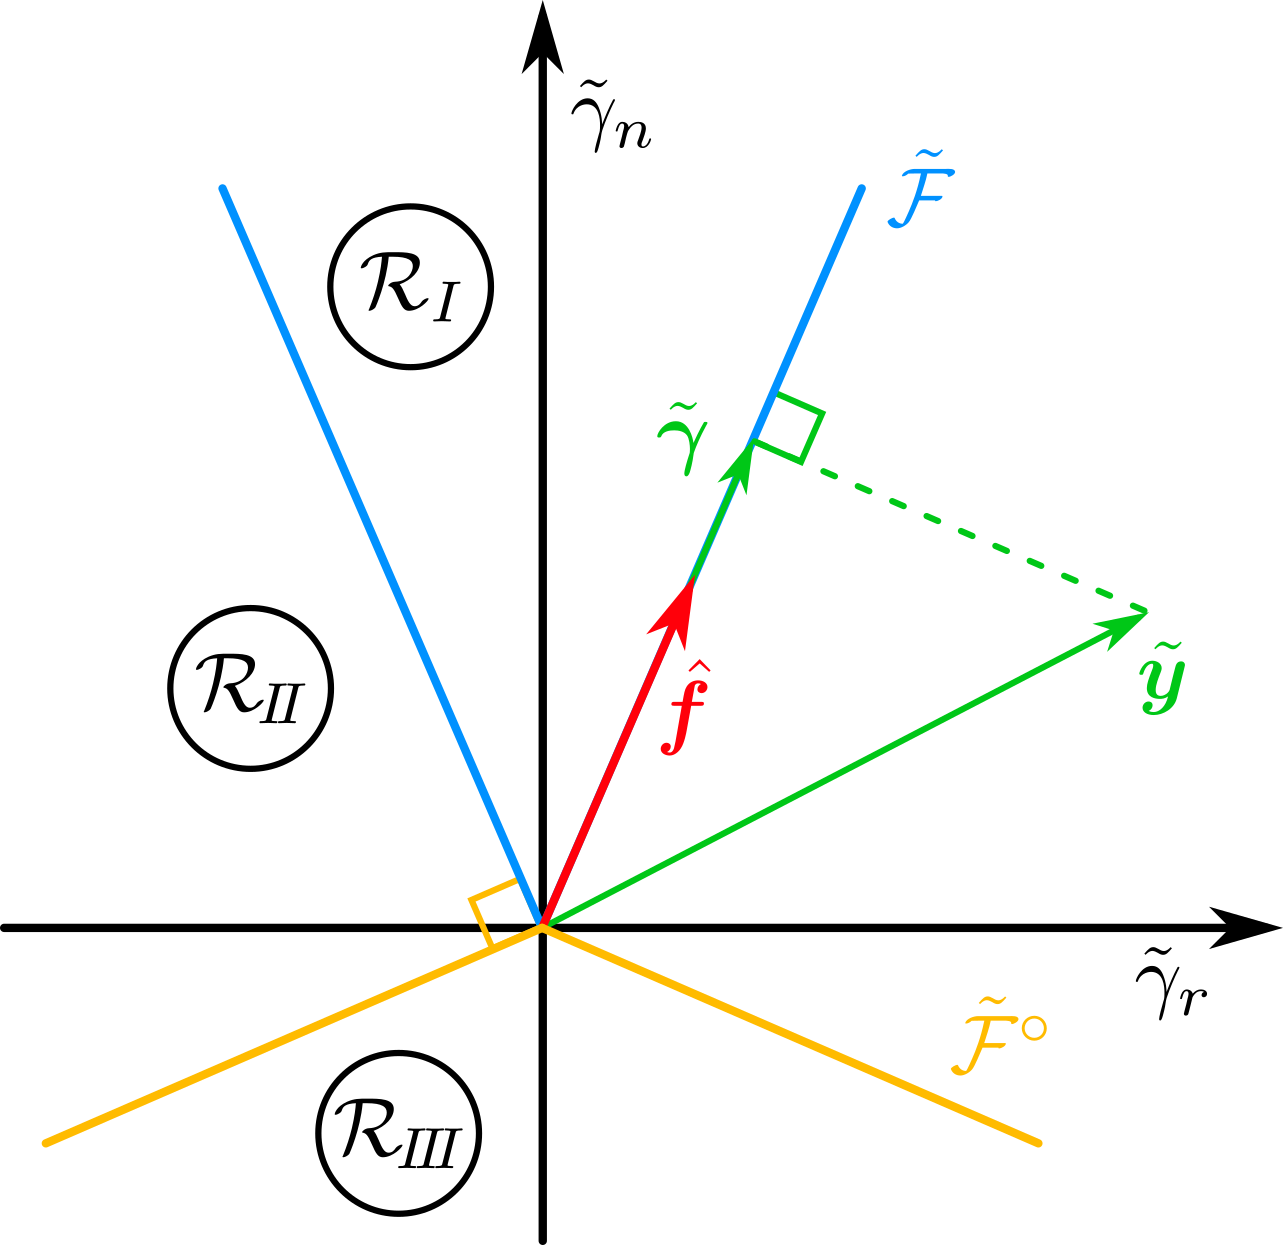
\includegraphics[width=0.6\columnwidth]{figures/schematics/analytical_inverse_dynamics.png}
    \caption{Geometry of the projection and regions in the
    $\tilde{\vf{y}}$ space.}
    \label{fig:cone_regions}
\end{figure}

Finally, we apply the inverse transformation
$\bgamma=\mf{R}^{-1/2}P_{\tilde{\mathcal{F}}}(\tilde{\vf{y}})$ and after some
algebraic manipulation we recover the projection $\bgamma =
P_\mathcal{F}(\vf{y})$ in Eq. \eqref{eq:analytical_y_projection}.




\section{Computation of the Gradients}
\label{app:gradients_derivation}
We first write the regularization term as
\begin{eqnarray*}
	\ell_R = \frac{1}{2}\Vert\bgamma\Vert_R^2=\frac{1}{2}(R_t\Vert\bgamma_t\Vert^2+R_n\gamma_n^2).
\end{eqnarray*}

In \textbf{stiction} $\bgamma=\vf{y}$ and the cost can be written as
\begin{eqnarray*}
	\ell_R(\vf{y}) = \frac{1}{2}(R_t y_r^2+R_n y_n^2).
\end{eqnarray*}

During \textbf{sliding} Eq. (\ref{eq:analytical_y_projection}) states that Coulomb's law applies and we can write
\begin{align*}
	\ell_R(\vf{y})
	&=\frac{1}{2}\gamma_n^2(R_t\mu^2+R_n)\\
	&=\frac{R_n}{2}(1+\tilde\mu^2)\gamma_n^2\\
	&=\frac{R_n}{2(1+\tilde\mu^2)}\left(y_n + \hat\mu y_r\right)^2,
\end{align*}
with $\tilde{\mu}=\mu (R_t/R_n)^{1/2}$ and $\hat{\mu}=\mu R_t/R_n$. Finally when there is \textbf{no contact}
\begin{eqnarray*}
	\ell_R(\vf{y}) = 0
\end{eqnarray*}

Therefore $\ell_R$ is the piecewise function
\begin{align}
	&\ell_R(\vf{y}) = 
	\label{eq:ell_R_piecewise}\\	
&\begin{dcases}
	% Region I, stiction
	\frac{1}{2}(R_t y_r^2+R_n y_n^2) & \text{stiction, } y_r \le \mu y_n\\
	% Region II, sliding.
	\frac{R_n}{2(1+\tilde\mu^2)}\left(y_n + \hat\mu y_r\right)^2 & \text{sliding, } -\hat\mu y_r < y_n \leq \frac{y_r}{\mu}\\
	% Region II, no contact.
    \vf{0} & \text{no contact, } y_n < -\hat\mu y_r
\end{dcases}\nonumber	
\end{align}

As discussed at the end of Appendix
\ref{app:analytical_inverse_dynamics_derivations}, in practice we use the
\emph{soft-norm} to define $y_r=\Vert\vf{y}_t\Vert_s$ so that $y_r$ is
differentiable at $\vf{y}=\vf{0}$.

\subsection{Gradients per Contact Point}
In this section we compute the gradients of $\ell_R(\mf{y})$ with respect to the
$i\text{-th}$ contact point variable $\vf{y}_i\in\mathbb{R}^3$. Unless otherwise
stated, we'll drop the subindex $i$. Therefore in this section $\nabla_\vf{y}\ell_R\in\mathbb{R}^3$ and
$\nabla_\vf{y}^2\ell_R\in\mathbb{R}^{3\times 3}$ (notice that as per our
notation, we consistently use a bold italic font for 3D vectors and only bold,
not italic, for $n\text{-dimensional}$ vectors.) The full gradient
$\nabla_\mf{y}\ell_R$ concatenates the three-dimensional gradients
$\nabla_\vf{y}\ell_R$ while the full Hessian matrix is block-diagonal with each
$3\times 3$ block containing the local $i\text{-th}$ point Hessian. This is
particularly useful to exploit sparsity in the computations.

We use the following identities to simplify expressions
\begin{eqnarray}
	\frac{\partial y_r}{\partial\vf{y}_t} &=& \hat{\vf{t}}\nonumber\\
	\frac{\partial \hat{\vf{t}}}{\partial\vf{y}_t} &=&
	\frac{\vf{P}^\perp(\hat{\vf{t}})}{y_r}
	\label{eq:yt_derivatives}
\end{eqnarray}
where the $2\times 2$ projection matrices along and perpendicular to
$\hat{\vf{t}}$ are defined as
\begin{eqnarray}
	\vf{P}(\hat{\vf{t}}) &=& \hat{\vf{t}}\otimes\hat{\vf{t}}\nonumber\\
	\vf{P}^\perp(\hat{\vf{t}})&=&\vf{I}_2 - \vf{P}(\hat{\vf{t}})
	\label{eq:tangential_projections}
\end{eqnarray}
and we note that Eqs. \eqref{eq:yt_derivatives} and
\eqref{eq:tangential_projections} are exactly valid when using our soft-norm to
define $y_r$.

Taking the gradient of Eq. (\ref{eq:ell_R_piecewise}) results in
\begin{align}
	&\nabla_\vf{y}\ell_R(\vf{y}) = 
	\label{eq:gradient_ell_R_piecewise}\\
&\begin{dcases}
	%%%%%%%%%%%%%%%%%%%%
	% Region I, stiction
	\vf{R}\,\vf{y} & 
	% when,
	\text{stiction, } y_r \le \mu y_n\\
	%
	%%%%%%%%%%%%%%%%%%%%
	% Region II, sliding.
	\frac{1}{1+\tilde\mu^2}\hat{s}^\circ(\vf{y})\begin{bmatrix}
		\mu R_t\hat{\vf{t}}\\
		R_n\\
	\end{bmatrix} &
	% when,
	\text{sliding, } -\hat\mu y_r < y_n \leq \frac{y_r}{\mu}\\
	% Region II, no contact.
    \vf{0} & \text{no contact, } y_n < -\hat\mu y_r
\end{dcases}\nonumber
\end{align}
with $\hat{s}^\circ(\vf{y}) = \hat{\mu}y_r+y_n$. $\hat{s}^\circ(\vf{y})$, a
measure of how close the solution is to the polar cone $\mathcal{F}^\circ$.
$\hat{s}^\circ(\vf{y}) > 0$ in the sliding region and $\hat{s}^\circ<0$ when
there is no contact.

Similarly, we can compute the Hessian of $\ell_R$ by taking the gradient in Eq.
(\ref{eq:gradient_ell_R_piecewise})
\begin{align}
	&\nabla_\vf{y}^2\ell_R(\vf{y}) = 
	\label{eq:hessian_ell_R_piecewise}\\
&\begin{dcases}
	%%%%%%%%%%%%%%%%%%%%
	% Region I, stiction
	\vf{R} & 
	% when,
	\text{stiction,}\\
	%
	%%%%%%%%%%%%%%%%%%%%
	% Region II, sliding.
	\frac{R_n}{1+\tilde\mu^2}
	\begin{bmatrix}
		% ∂²ℓ/∂yₜ²:
		\hat{\mu}\left(\hat{\mu}\vf{P}(\hat{\vf{t}})+\hat{s}^\circ(\vf{y})\vf{P}^\perp(\hat{\vf{t}})/y_r\right) & 
		% ∂²ℓ/∂yₙ∂yₜ:
		\hat{\mu}\vf{t}\\
		% ∂²ℓ/∂yₜ∂yₙ:
		\hat{\mu}\vf{t}^T & 
		% ∂²ℓ/∂yₙ²:
		1\\
	\end{bmatrix} &
	% when,
	\text{sliding,}\\
	% Region II, no contact.
    \vf{0} & \text{no contact.}
\end{dcases}\nonumber
\end{align}

Clearly in the stiction region we have $\nabla_\vf{y}^2\ell_R(\vf{y})\succ 0$.
Since in the stiction region we have $\hat{s}^\circ(\vf{y})>0$, the linear
combination of $\vf{P}(\hat{\vf{t}})$ and $\vf{P}(\hat{\vf{t}})^\perp$ in Eq.
(\ref{eq:hessian_ell_R_piecewise}) is PSD (since both projection matrices are
PSD). Therefore, in the sliding region we find out that
$\nabla_\vf{y}^2\ell_R(\vf{y})\succeq 0$.

Finally, we note that we are using a slight abuse of notation. The Hessian of
the regularizer does not exist at points on the boundary of $\mathcal{F}$ nor at
points on the boundary of $\mathcal{F}^\circ$. What we are really doing is
analytically \emph{extending} the Hessian on those points; on the boundary of
$\mathcal{F}$ we extend the stiction solution and on the boundary of
$\mathcal{F}^\circ$ we extend the no contact solution.

\subsection{Gradients with Respect to Velocities}
These gradients are computed using the chain rule and the definition of $\mf{y}$
\begin{equation*}
	\mf{y}=-\mf{R}^{-1}(\mf{J}\mf{v} - \hat{\mf{v}}_c)
\end{equation*}

Therefore the gradient in terms of velocities is
\begin{equation}
	\nabla_\mf{v}\ell_R = -\mf{J}^T\mf{R}^{-1}\nabla_\mf{y}\ell_R
	\label{eq:ell_velocity_gradient}
\end{equation}
which, using Eq. (\ref{eq:gradient_ell_R_piecewise}), can be written as
\begin{equation}
	\nabla_\mf{v}\ell_R = -\mf{J}^T\bgamma
	\label{eq:ell_velocity_gradient_simplified}
\end{equation}

We obtain the Hessian of the regularizer $\ell_R(\mf{v})$ from the
gradients of $\bgamma(\mf{v})$ in Eq. \eqref{eq:ell_velocity_gradient_simplified}
\begin{eqnarray}
	\nabla_\mf{v}^2\ell_R(\mf{v}) &=& \mf{J}^T\mf{G}\,\mf{J}\nonumber\\
	\mf{G} &=&-\nabla_{\mf{v}_c}\bgamma = \nabla_\mf{y}\bgamma \mf{R}^{-1}
	\label{eq:ellR_hessian}
\end{eqnarray}
where $\nabla_{\mf{v}_c}\!\bgamma$ is a block diagonal matrix where each
diagonal block is the $3\times 3$ matrix $\nabla_{\mf{v}_{c,i}}\!\bgamma_i$
for the $i\text{-th}$ contact.

Alternatively, taking the gradient of Eq. \eqref{eq:ell_velocity_gradient} leads to the equivalent result
\begin{equation}
	\nabla_\mf{v}^2\ell_R = \mf{J}^T\mf{R}^{-1}\nabla_\mf{y}^2\ell_R\mf{R}^{-1}\mf{J}
	\label{eq:ell_velocity_hessian}
\end{equation}
and since we already showed $\nabla_\mf{y}^2\ell_R\succeq 0$, it follows that
$\nabla_\mf{v}^2\ell_R\succeq 0$.


\subsection{Gradients of the Primal Cost}
With these results, we can now write the gradient and Hessian of the primal cost
$\ell_p(\mf{v})$ in Eq. (\ref{eq:primal_unconstrained}). For the gradient we
have
\begin{equation}
	\nabla_\mf{v}\ell_p(\mf{v}) = \mf{A}(\mf{v}-\mf{v}^*) + \nabla_\mf{v}\ell_R
\end{equation}

Notice that, using Eq. (\ref{eq:ell_velocity_gradient_simplified}), the gradient
can be written as
\begin{equation}
	\nabla_\mf{v}\ell_p(\mf{v}) = \mf{A}(\mf{v}-\mf{v}^*) - \mf{J}^T\bgamma
\end{equation}
and since the unconstrained minimization looks for $\nabla_\mf{v}\ell_p=\mf{0}$,
we essentially recover the balance of momentum, as expected.

Similarly, we can write the Hessian as
\begin{equation}
	\mf{H} = \nabla_\mf{v}^2\ell_p(\mf{v}) = \mf{A} + \nabla_\mf{v}^2\ell_R
\end{equation}
and since we already proved that $\nabla_\mf{v}^2\ell_R\succeq 0$, we find that
 $\mf{H}\succ 0$. Finally, we observe we are using the same analytical
 extensions used to defined $\nabla_\mf{v}^2\ell_R$ at points of
 non-differentiability.


\section{Convergence Analysis of SAP}
\label{app:sap_converge}
\newcommand{\coneName}{\mathcal{K}}
\newcommand{\dist}{d}
\newcommand{\cond}{\text{cond}}
\newcommand{\vx}{\mf{v}}
\newcommand{\fx}{\ell_p(\mf{\vx})}

\newcommand{\vy}{\mf{u}}
\newcommand{\fy}{\ell_p(\mf{\vy})}
\newcommand{\vd}{\mf{d}}

% As required by the IEEE template.
\renewcommand\qedsymbol{$\IEEEQED$}

Convergence of SAP is established
by first showing that the objective function 
$\ell_p(\mf{v}) = \frac{1}{2}\Vert\mf{v}-\mf{v}^*\Vert_{A}^2 + P_\mathcal{F}(\mf{y}(\mf{v}))\Vert_R^2$
is \emph{strongly convex}
and differentiable with \emph{Lipschitz continuous} gradients.  The
former property is inherited from the positive-definite quadratic term 
provided by the positive definite matrix $\mf{A}$ in Eq. \eqref{eq:primal_unconstrained}.  The latter is shown using differentiability of the squared-distance function
 and the Lipschitz continuity of its gradient map (Theorems 5.3-i 6.1-i of~\cite{bib:delfour2011shapes})
 combined with the identity
\[
  \dist^2_{\coneName^\circ}(x) = \|P_{\coneName}(x)\|_{\mf{R}}^2,
\] 
for any closed, convex cone $\coneName$. Here 
the distance and projection functions are with respect to the
norm $\|\cdot\|_\mf{R}$, while $\coneName^\circ$ denotes the polar
cone with respect to the corresponding inner-product $\mf{x}^T \mf{R} \mf{y}$.
\begin{lemma}\label{lem:PropertiesOfObj}
  The following statements hold.
  \begin{itemize}
    \item The function $\fx$ is strongly convex, i.e., there exists $\mu >0$
      such that 
      \[
        \fy \ge \fx + \nabla \fx(\vy-\vx) + \frac{\mu}{2} \|\vy-\vx\|^2
      \]
    \item The function $\fx$ is differentiable and has Lipschitz continuous gradients, i.e.,
      $\nabla \fx$ exists for all $\mf{v}$ and there exists $L \ge 0$ satisfying
      \[
      \|\nabla \fx - \nabla \fy\| \le L \|\vy - \vx\|
      \]
  \end{itemize}
  \begin{proof}

The objective $\fx$ is a function $f : \mathbb{R}^n \rightarrow \mathbb{R}$
of the following form
\[
  f(\vx) = \frac{1}{2}\dist_{\coneName}^2(\mf{Z}\vx + \mf{b}) + \vx^{T}\mf{W}\vx + \mf{q}^T \vx,
\]
where $\mf{Z} \in \mathbb{R}^{m \times n}$, $\mf{W} \in \mathbb{R}^{n \times n}$ is
symmetric and positive definite, and $\dist_{\coneName} : \mathbb{R}^{m} \rightarrow \mathbb{R}$ 
denotes the distance function of a closed, convex set $\coneName \subseteq \mathbb{R}^m$
as measured by some quadratic norm $\|\mf{x}\|_Q$, i.e.,
\[
  \dist_{\coneName}(\vx) = \inf \{ \|\vx-\mf{z}\|_Q : \mf{z} \in \coneName\}.
\]
    The sum of a strongly convex function with a convex function is strongly
    convex.  Since the squared distance function is convex, and the quadratic
    term $\vx^T \mf{W}\vx$ is strongly convex (given that $\mf{W} \succ 0$), the  first
    statement holds.

    The second statement follows trivially if we can show it holds 
    for the squared distance function. 
    Differentiability follows from Chapter 4 (Theorems 5.3-i 6.1-i) of~\cite{bib:delfour2011shapes},
    which shows that
  \[
    \nabla \dist_{\coneName}^2(\vx) = 2 \mf{Q} (\vx - P_{\coneName}(\vx)).
  \]
    That the gradient of $\dist_{\coneName}^2(\vx)$ is Lipschitz follows
    from Lipschitz continuity of projection maps onto closed, convex sets.
  \end{proof}
\end{lemma}
\noindent We remark that strong convexity implies the reverse
Lipschitz inequality $\|\nabla f(\vx) - \nabla f(\vy)\| \ge \mu \|\vx - \vy\|$,
which in turn means that the parameter $\mu$ and the Lipschitz constant $L$
satisfy $\mu \le L$.




Recall that SAP (Algorithm~\ref{alg:sap}) is a special case
of the following iterative method
for minimizing a function $f : \mathbb{R}^n \rightarrow
\mathbb{R}$ given some initial
point $\vx_0 \in \mathbb{R}^n$:
\begin{align}\label{eq:quasiNewtonIter}
  \begin{aligned}
    \vd_m &= -\mf{H}^{-1}(\vx_m) \nabla f(\vx_m), \\
     t_m &= \argmin_{t} f(\vx_m + t \vd_m),\\
    \vx_{m+1} &= \vx_m + t_m \vd_m,      
  \end{aligned}
\end{align}
where $\mf{H} : \mathbb{R}^n \rightarrow \mathbb{R}^{n \times n}$ is a function 
into the set of symmetric positive definite matrices, i.e.,  $\mf{H}(\vx) = \mf{H}(\vx)^T$ 
and $\mf{H}(\vx) \succ 0$ for all $\vx\in\mathbb{R}^n$.  
It is well known that gradient descent exhibits linear convergence to the global minimum when applied to a strongly convex
function with Lipschitz continuous gradient. Incorporating
a condition number bound  $\sigma$ for $\mf{H}(\vx)$  into standard gradient-descent analysis
will prove that the iterations~\eqref{eq:quasiNewtonIter}
also have linear convergence.
To show this, we let
$\cond(\mf{H}(\vx))$ denote the condition number of $\mf{H}(\vx)$
and $S(\vx_0)$ denote the sub-level set $\{ \vx \in \mathbb{R}^n: f(\vx) \le f(\vx_0) \}$.
\begin{lemma}\label{lem:GlobalConv}
  Let $f : \mathbb{R}^n \rightarrow \mathbb{R}$ be strongly convex and differentiable
  with Lipschitz-continuous gradients.
  Fix $\vx_0 \in\mathbb{R}^n$. If there exists $\sigma > 0$
  such that $\cond(\mf{H}(\vx)) \le \sigma$ for all  $\vx \in S(\vx_0)$, then
  the iterations~\eqref{eq:quasiNewtonIter}
  converge to the global minimum $\vx_*$ of $f(\vx)$ when initialized at $\vx_0$.
  Moreover,
  \[
    f(\vx_m)  - f(\vx_*)  \le (1-\frac{\mu}{\sigma^2 L})^m (f(\vx_0) - f(\vx_*))
  \]
  for all iterations $m$, where $\mu$ is the strong-convexity parameter of $f(\vx)$ and $L$ is
  the Lipschitz constant of $\nabla f(\vx)$.
  \begin{proof}
    Dropping the subscript $m$ from $(\vx_m, t_m, \vd_m)$, we first observe that
\[
f(\vx+t\vd) \le f(\vx) + \langle \nabla f(\vx), \vd \rangle t + \frac{L}{2}\|\vd\|^2 t^2,
\]
by Lipschitz continuity.  Substituting $\vd =- \mf{H}^{-1}  \nabla  f(\vx)$ gives
\[
f(\vx+t\vd) = f(\vx) - \nabla f(\vx)^T  \mf{H}^{-1}  \nabla  f(\vx) t + \frac{L }{2}\|\mf{H}^{-1}\nabla f(\vx) \|^2 t^2.
\]
Letting $\lambda_{max}$ and $\lambda_{min}$ denote the
maximum and minimum eigenvalues of $\mf{H}$ evaluated at $\vx$, it also follows that
\[
  f(\vx+t\vd) \le f(\vx) - \frac{1}{\lambda_{\max}} \|\nabla f(\vx)\|^2 t  + 
    \frac{L }{2}  \frac{1}{\lambda^{2}_{\min}} \|\nabla f(\vx)\|^2 t^2.
\]
Letting $\bar t$ denote the  minimizer of the right-hand-side, we
conclude that
    \[
      f(\vx+t\vd) \le  f(\vx + \bar t\vd ) \le f(\vx) - \frac{1}{2}(\frac{\lambda^{2}_{\min}}{\lambda^2_{\max} L} 
      \|\nabla f(\vx)\|^2),
    \]
where the first inequality follows from the exact line search
used to select $t$.
Since  $\sigma^2 \ge \lambda^{2}_{\max}/\lambda^2_{\min}$,
we conclude that
\[
   f(\vx + t \vd) \le f(\vx) - \frac{1}{2\sigma^2 L}\| \nabla f(\vx) \|^2.
\]
    On the other hand, letting $f_* = f(\vx_*)$ 
    we have from strong convexity that the Polyak-Lojasiewicz
    inequality holds:
    \[
  \|\nabla f(\vx)\|^2 \ge 2\mu (f(\vx)-f_* ).
    \]
Hence,
\[
  f(\vx + t \vd)   \le f(\vx) - \frac{\mu}{\sigma^2 L} (f(\vx)-f_* ).
\]
Subtracting $f_*$ from both sides and factoring shows
\[
  f(\vx + t \vd)  - f_* \le  (1-\frac{\mu}{\sigma^2 L})(f(\vx) - f_*).
\]
It follows that each iteration $m$ satisfies
\[
  f(\vx_{m+1}) - f_* \le  (1-\frac{\mu}{\sigma^2 L})^{m}(f(\vx_{0}) - f_*).
\]
Since $\sigma \ge 1$ and $L \ge \mu$, the iterations converge, and the proof is completed.
  \end{proof}
\end{lemma}

Combining these lemmas shows that SAP globally convergences at (at least) a
linear rate.  By observing that SAP reduces to Newton's
method when the gradient is differentiable, we can also prove local quadratic
convergence assuming differentiability on a neighborhood of
the optimum $\vx_*$. 
\begin{theorem}
  The following statements hold.
  \begin{itemize}
    \item SAP globally converges from all initial conditions.
    \item If $\nabla f(\vx)$  is differentiable on the ball $B(\vx_*, r) := \{ \vx :  \|\vx-\vx_*\| \le r\}$
  for some $r > 0$, then SAP exhibits quadratic convergence, i.e., for some finite
  $M$ and $\zeta > 0$
  \[
    \|\vx_m - \vx_*\| \le \zeta \|\vx_{m+1} - \vx_*\|^2
  \]
  for all $m > M$.
  \end{itemize}

  \begin{proof}

    The first statement follows from Lemmas~\ref{lem:PropertiesOfObj}~and~\ref{lem:GlobalConv}.

  To prove the second, we show that $B(\vx_*, r)$
    contains a sublevel set $\Omega_{\beta} = \{ \vx : f(\vx) \le \beta\}$ for some
  $\beta > 0$,  implying that SAP 
  reduces to Newton's method with exact line search for some $m > M$,
 given that sublevel sets are invariant. 

  To begin, we have, by strong convexity, that
  \begin{equation}
    \beta \ge f(\vx) \ge f(\vx_*)  + \frac{\mu}{2} \|\vx-\vx_*\|^2,
    \label{eq:strong_convexity_at_differentiable_optimal}
  \end{equation}
    for all $\vx \in \Omega_{\beta}$.
    Rearranging shows that
    \[
      \|\vx-\vx_*\|^2 \le 2\frac{\beta- f(\vx_*)}{\mu}.
    \]
    Hence, $B(\vx_*, r)$ contains
    $\Omega_{\beta}$ for any $\beta$ satisfying $2\frac{\beta- f(\vx_*)}{\mu} < r$.
    For some finite $M$, we also have that $v_m \in \Omega_{\beta}$ for all $m > M$ 
    by Lemma~\ref{lem:GlobalConv}.

    Next, we prove that Newton iterations are quadratically convergent
  with exact line search. Indeed, using once more the strong convexity result in Eq.~\eqref{eq:strong_convexity_at_differentiable_optimal}
  \begin{align*}
    \|\vx_{m+1} - \vx_*\|^2&\le \frac{2}{\mu} ( f(\vx_{m+1}) - f(\vx_*)) \\
                    &= \frac{2}{\mu} ( f(\vx_m + t_m \vd_m   ) - f(\vx_*)) \\
                    &\le \frac{2}{\mu} ( f(\vx_m + \vd_m   ) - f(\vx_*)) \\
                    &\le \frac{2}{\mu} L \|\vx_m + \vd_m - \vx_*\|^2,
  \end{align*}
    where the first line uses strong convexity,
    the third exact line search, and the last
    Lipschitz continuity. But for some $\kappa > 0$,
    we have that $\|\vx_m + \vd_m - \vx_*\|^2 \le \kappa \|\vx_{m} - \vx_*\|^4$
    by quadratic convergence of Newton's method with unit step-size (\cite[Theorem 3.5]{bib:nocedal2006numerical}).
    Hence,
    \[
      \|\vx_{m+1} - \vx_*\|^2 \le \frac{2}{\mu}  L \kappa \|\vx_{m} - \vx_*\|^4,
    \]
    and the claim is proven.
  \end{proof}
\end{theorem}




% use section* for acknowledgment
\section*{Acknowledgment}
The authors would like to thank...

% An example of a floating figure using the graphicx package.
% Note that \label must occur AFTER (or within) \caption.
% For figures, \caption should occur after the \includegraphics.
% Note that IEEEtran v1.7 and later has special internal code that
% is designed to preserve the operation of \label within \caption
% even when the captionsoff option is in effect. However, because
% of issues like this, it may be the safest practice to put all your
% \label just after \caption rather than within \caption{}.
%
% Reminder: the "draftcls" or "draftclsnofoot", not "draft", class
% option should be used if it is desired that the figures are to be
% displayed while in draft mode.
%
%\begin{figure}[!t]
%\centering
%\includegraphics[width=2.5in]{myfigure}
% where an .eps filename suffix will be assumed under latex, 
% and a .pdf suffix will be assumed for pdflatex; or what has been declared
% via \DeclareGraphicsExtensions.
%\caption{Simulation results for the network.}
%\label{fig_sim}
%\end{figure}

% Note that the IEEE typically puts floats only at the top, even when this
% results in a large percentage of a column being occupied by floats.


% An example of a double column floating figure using two subfigures.
% (The subfig.sty package must be loaded for this to work.)
% The subfigure \label commands are set within each subfloat command,
% and the \label for the overall figure must come after \caption.
% \hfil is used as a separator to get equal spacing.
% Watch out that the combined width of all the subfigures on a 
% line do not exceed the text width or a line break will occur.
%
%\begin{figure*}[!t]
%\centering
%\subfloat[Case I]{\includegraphics[width=2.5in]{box}%
%\label{fig_first_case}}
%\hfil
%\subfloat[Case II]{\includegraphics[width=2.5in]{box}%
%\label{fig_second_case}}
%\caption{Simulation results for the network.}
%\label{fig_sim}
%\end{figure*}
%
% Note that often IEEE papers with subfigures do not employ subfigure
% captions (using the optional argument to \subfloat[]), but instead will
% reference/describe all of them (a), (b), etc., within the main caption.
% Be aware that for subfig.sty to generate the (a), (b), etc., subfigure
% labels, the optional argument to \subfloat must be present. If a
% subcaption is not desired, just leave its contents blank,
% e.g., \subfloat[].


% An example of a floating table. Note that, for IEEE style tables, the
% \caption command should come BEFORE the table and, given that table
% captions serve much like titles, are usually capitalized except for words
% such as a, an, and, as, at, but, by, for, in, nor, of, on, or, the, to
% and up, which are usually not capitalized unless they are the first or
% last word of the caption. Table text will default to \footnotesize as
% the IEEE normally uses this smaller font for tables.
% The \label must come after \caption as always.
%
%\begin{table}[!t]
%% increase table row spacing, adjust to taste
%\renewcommand{\arraystretch}{1.3}
% if using array.sty, it might be a good idea to tweak the value of
% \extrarowheight as needed to properly center the text within the cells
%\caption{An Example of a Table}
%\label{table_example}
%\centering
%% Some packages, such as MDW tools, offer better commands for making tables
%% than the plain LaTeX2e tabular which is used here.
%\begin{tabular}{|c||c|}
%\hline
%One & Two\\
%\hline
%Three & Four\\
%\hline
%\end{tabular}
%\end{table}


% Note that the IEEE does not put floats in the very first column
% - or typically anywhere on the first page for that matter. Also,
% in-text middle ("here") positioning is typically not used, but it
% is allowed and encouraged for Computer Society conferences (but
% not Computer Society journals). Most IEEE journals/conferences use
% top floats exclusively. 
% Note that, LaTeX2e, unlike IEEE journals/conferences, places
% footnotes above bottom floats. This can be corrected via the
% \fnbelowfloat command of the stfloats package.

% if have a single appendix:
%\appendix[Proof of the Zonklar Equations]
% or
%\appendix  % for no appendix heading
% do not use \section anymore after \appendix, only \section*
% is possibly needed

% use appendices with more than one appendix
% then use \section to start each appendix
% you must declare a \section before using any
% \subsection or using \label (\appendices by itself
% starts a section numbered zero.)
%

% Can use something like this to put references on a page
% by themselves when using endfloat and the captionsoff option.
\ifCLASSOPTIONcaptionsoff
  \newpage
\fi



% trigger a \newpage just before the given reference
% number - used to balance the columns on the last page
% adjust value as needed - may need to be readjusted if
% the document is modified later
%\IEEEtriggeratref{8}
% The "triggered" command can be changed if desired:
%\IEEEtriggercmd{\enlargethispage{-5in}}

% references section

% can use a bibliography generated by BibTeX as a .bbl file
% BibTeX documentation can be easily obtained at:
% http://mirror.ctan.org/biblio/bibtex/contrib/doc/
% The IEEEtran BibTeX style support page is at:
% http://www.michaelshell.org/tex/ieeetran/bibtex/
%\bibliographystyle{IEEEtran}
% argument is your BibTeX string definitions and bibliography database(s)
%\bibliography{IEEEabrv,../bib/paper}
%
% <OR> manually copy in the resultant .bbl file
% set second argument of \begin to the number of references
% (used to reserve space for the reference number labels box)
\bibliographystyle{./IEEEtran/IEEEtran}
\bibliography{./IEEEtran/IEEEabrv,sap_paper}

% biography section
% 
% If you have an EPS/PDF photo (graphicx package needed) extra braces are
% needed around the contents of the optional argument to biography to prevent
% the LaTeX parser from getting confused when it sees the complicated
% \includegraphics command within an optional argument. (You could create
% your own custom macro containing the \includegraphics command to make things
% simpler here.)
%\begin{IEEEbiography}[{\includegraphics[width=1in,height=1.25in,clip,keepaspectratio]{mshell}}]{Michael Shell}
% or if you just want to reserve a space for a photo:

% that's all folks
\end{document}


